\documentclass[italian]{notes}

\usepackage{mama}

\title{Analisi Funzionale}
\author{Matteo Capucci (sul corso del prof. Lamberti)}
\date{a.a. 2019/2020}

\addbibresource{./bibliography.bib}

\renewcommand{\L}{\mathcal{L}}
\newcommand{\supp}{\operatorname{supp}}
\newcommand{\dist}{\operatorname{dist}}
\newcommand{\M}{\mathcal{M}}
\newcommand{\esssup}{\operatorname{ess\,supp}}
\newcommand{\sgn}{\operatorname{sgn}}
\newcommand{\dx}{\mathrm{d}x}
\newcommand{\dt}{\mathrm{d}t}

\newcommand{\weakconv}{\rightharpoonup}
\renewcommand{\conv}[1][]{\underset{{#1}}{\rightarrow}}

\begin{document}
	\maketitle

	\tableofcontents

	\chapter{Operatori lineari e continui}
Ricordo che uno spazio normato su $\R$ (o $\C$) è uno spazio vettoriale $E$ su $\R$ (o $\C$) munito di una norma, cioè una funzione
$$
	\| - \|_E : E \to [0,+\infty)
$$
tale che
\begin{enumerate}
	\item per ogni $x \in E$, $\|x\|_E = 0 \sse x=0$,
	\item per ogni $x \in E$, $\lambda \in \R$ (o $\C$), $\|\lambda x \|_E = |\lambda|\|x\|_E$,
	\item per ogni $x,y \in E$, $\|x + y\|_E \leq \|x\|_E + \|y\|_E$.
\end{enumerate}
La norma definisce una distanza
$$
	d_E(x,y) = \|x-y\|_E, \qquad \forall x, y \in E
$$
che rende $E$ uno spazio metrico: per ogni $x,y,z \in E$,
\begin{enumerate}
	\item $d_E(x,y) = 0 \sse x=y$,
	\item $d_E(x,y) = d_E(y,x)$,
	\item $d_E(x,y) + d_E(y,z) \leq d_E(x,z) + d_E(z,y)$.
\end{enumerate}
Se $(E, d_E)$ è completo come spazio metrico, $(E, \|-\|_E)$ si dice \defining{spazio di Banach}.

\begin{lemma}
\label{lemma:reverse_triang_ineq}
	In uno spazio normato, vale la disuguglianza
	\begin{equation}
		\|x-y\| \geq \|x\|-\|y\|
	\end{equation}
\end{lemma}

\begin{theorem}
	Siano $E$, $F$ spazi normati e $T: E \to F$ una funziona lineare. Allora sono equivalenti le seguenti affermazioni:
	\begin{enumerate}
		\item $T$ è continua,
		\item $T$ è continua in un punto $x_0 \in E$,
		\item $T$ è continua in $0$,
		\item esiste $C > 0$ tale che
		$$
			\|Tx\|_F \leq C \|x\|_E, \qquad \forall x \in E.
		$$
	\end{enumerate}
	In tali casi si dice che $T$ è un \defining{operatore (lineare) limitato}.
\end{theorem}
\begin{proof}
	\leavevmode
	\begin{description}
		\item[$(1) \implies (2)$] Ovvio.
		\item[$(2) \implies (3)$] La continuità in $x_0$ singifica che per ogni $\varepsilon > 0$ esiste $\delta > 0$ tale che
		$$
			\|x-x_0\|_E < \delta \implies \|Tx - Tx_0\|_F < \varepsilon.
		$$
		Posto $y = x-x_0$, ciò comporta che
		$$
			\|y\|_E < \delta \implies \|Ty\| = \|Tx - Tx_0\|_F < \varepsilon
		$$
		ossia $T$ è continuo in $0$ (siccome ogni vettore $y$ di $E$ si può scrivere nella forma $x-x_0$ per un opportuno $x \in E$).
		\item[$(3) \implies (4)$] Per ogni $\varepsilon > 0$ esiste $\delta > 0$ tale che
		$$
			\|y\|_E < \delta \implies \|Ty\|_F < \varepsilon.
		$$
		Sia $x \in E$, $x \neq 0$. Poniamo
		$$
			y = \frac{x}{\|x\|_E}\frac{\delta}2
		$$
		Si ha $\|Ty\|_F < \varepsilon$, ossia
		$$
			\frac{\delta}{2\|x\|_E} \|Tx\|_F < \varepsilon
		$$
		da cui
		$$
			\|Tx\|_F < \frac{2\varepsilon}{\delta} \|x\|_E, \qquad \forall x \in E.
		$$
		\item[$(4) \implies (1)$] Sia $x_0 \in E$ fissato. Per ogni $x \in E$, sappiamo che
		$$
			\|T(x-x_0)\|_F \leq C \|x-x_0\|_E
		$$
		per una qualche costante $C > 0$. Sia $\varepsilon > 0$, e poniamo $\delta := \varepsilon/C$. Se $\|x-x_0\| < \delta allora$, si ha
		$$
			\|Tx - Tx_0\|_F = \|T(x-x_0)\|_F \leq C\|x-x_0\|_E < \varepsilon
		$$
		cioè $T$ è continuo in $x_0$.
	\end{description}
\end{proof}

\begin{lemma}
	Siano $E$, $F$ spazi normati e $T:E \to F$ un operatore limitato. Allora:
	$$
		\inf\{C > 0 \suchthat \forall x \in E,\; \|Tx\|_F \leq C\|X\|_E \} \overset{(1)}= \sup_{x \neq 0} \frac{\|Tx\|_F}{\|x\|_E} \overset{(2)}= \sup_{\|x\|_E=1} \|Tx\|_F \overset{(3)}= \sup_{\|x\|_E \leq 1} \|Tx\|_F.
	$$
\end{lemma}
\begin{proof}
	\leavevmode
	\begin{description}
		\item[$(1)$] Ovvio.
		\item[$(2)$] Vale
		$$
			\frac{\|Tx\|_F}{\|x\|_E} = \left\| \frac{Tx}{\|x\|_E} \right\|_F = \left\|T\left(\frac{x}{\|x\|_E}\right)\right\|_F
		$$
		da cui segue l'uguaglianza cercata.
		\item[$(3)$] È ovvio che $\sup_{\|x\|_E=1} \|Tx\|_F \geq \sup_{\|x\|_E \leq 1} \|Tx\|_F$. D'altra parte:
		$$
			\sup_{\|x\|_E \leq 1} \|Tx\|_F \leq \sup_{0 < \|x\|_E \leq 1} \frac{\|Tx\|_F}{\|x\|_E} \leq  \sup_{x \neq 0} \frac{\|Tx\|_F}{\|x\|_E} = \sup_{\|x\|_E = 1} \|Tx\|_F.
		$$
	\end{description}
\end{proof}

\begin{definition}
	Siano $E$ ed $F$ spazi normati.
	\begin{enumerate}
		\item Si pone
		$$
			\L(E, F) := \{ T:E \to F \suchthat \text{$T$ è lineare e continuo}\}.
		$$
		\item Se $F=\R$ (o $\C$), allora si definisce
		$$
			E' = \L(E, F)
		$$
		il \defining{duale topologico} di $E$.
		\item Si pone
		$$
			\|T\|_{\L(E,F)} := \|T\|_{E \to F} := \sup_{x \neq 0} \frac{\|Tx\|_F}{\|x\|_E}.
		$$
	\end{enumerate}
\end{definition}

\begin{exercise}
	Provare che $\|-\|_{E \to F}$ definisce una norma su $\L(E,F)$.
\end{exercise}

\begin{remark}
	È vero che
	$$
		\|Tx\|_F \leq \|T\|_{E \to F} \|x\|_E, \qquad \forall x \in E,
	$$
	però in generale il $\sup$ che definisce $\|T\|_{E \to F}$ non è un max.
\end{remark}

\begin{example}
\label{ex:unif_deriv}
	Siano $E = \Cone[a,b]$, $F = \Czero[a,b]$, per $-\infty < a < b < +\infty$, entrambi muniti della norma della convergenza uniforme:
	$$
		\|x\|_E := \|x\|_F := \|x\|_\infty := \max_{t \in [a,b]} |x(t)|.
	$$
	Definiamo
	\begin{eqalign}
		T : \Cone[a,b] &\longto \Czero[a,b]\\
		x &\longmapsto Tx := \der{x}{t}
	\end{eqalign}
	$T$ è lineare ma non è continuo. Infatti la successione
	$$
		x_n(t) = \left(\frac{t-a}{b-a}\right)^n, \qquad t \in [a,b]
	$$
	è tale per cui
	$$
		\|x_n\|_\infty = 1, \qquad \left\|\der{x_n}{t}\right\|_\infty = \max_{t \in [a,b]} \left| n \left(\frac{t-a}{b-a}\right)^{n-1} \frac1{b-a} \right| = \frac{n}{b-a};
	$$
	cioè la successione $\{x_n\}_{n \in \N}$ è limitata mentre la sua immagine $\{\der{x_n}t\}_{n \in \N}$ non lo è!
\end{example}

\begin{question*}
	Cosa fare per rendere continuo $T : x \mapsto \der{x}{t}$?
\end{question*}

È sufficiente usare la `giusta' norma su $\Cone$, cioè
$$
	\|x\|_E = \|x\|_{\Cone[a,b]} = \|x\|_\infty + \left\|\der{x}{t}\right\|_\infty, \qquad \forall x \in E.
$$
Adesso è vero che
$$
	\|Tx\|_F = \left\|\der{x}{t}\right\|_\infty \leq \|x\|_\infty + \left\|\der{x}{t}\right\|_\infty = \|x\|_E
$$
ossia $T$ è limitato di norma $\|T\| \leq 1$.

In realtà la norma di $T$ è esattamente $1$. Infatti posto $x_n(t) = \exp(n(t-a))$, si ha
$$
	\frac{\|Tx_n\|_F}{\|x_n\|_E} = \frac{\left\|\der{x}{t}\right\|_\infty}{\|x_n\|_\infty + \left\|\der{x}{t}\right\|_\infty} = \frac{n\e^{n(b-a)}}{\e^{n(b-a)} + n\e^{n(b-a)}} \conv[n] 1.
$$
Si osservi che non esiste $x \in E$ non nullo tale che $\|Tx\|_F = \|x\|_E$.

\begin{remark}
	Per provare la discontinuità nell'Esempio~\ref{ex:unif_deriv} si sarebbe potuta usare anche la successione:
	$$
		x_n(t) = \frac{\sin (nt)}n, \qquad \forall t \in [a,b]
	$$
	la quale converge uniformemente a $0$ ma le cui derivate $\der{x_n}t = \cos(nt) \not\conv[n] 0$.
\end{remark}

\begin{example}
	Sia $\R[x]$ lo spazio dei polinomi su $\R$, normato con la norma uniforme su $[0,1]$. La funzione
	\begin{eqalign}
		T: \R[x] &\longto \R\\
		p &\longmapsto Tp := p(5)
	\end{eqalign}
	è lineare ma non continua. Infatti posto
	$$
		p_n(t) = t^n
	$$
	abbiamo $\|p_n\|_\infty = 1$, ma $Tx_n = 5^n \conv[n] \infty$. Cosa sarebbe successo se al posto di $5$ avessimo usato $1/2$?
\end{example}
\begin{example}
	Sia $E=\Czero_c[0,1]$ lo spazio delle funzioni reali su $[0,1]$ continue e a supporto compatto, normato con la norma uniforme. Sia
	\begin{eqalign}
		T: E &\longto \R\\
		x &\longmapsto Tx := \int_0^1 x(t)\,dt
	\end{eqalign}
	Essa è evidentemente lineare, ed è anche continua:
	$$
		|Tx\| \leq \int_0^1 |x(t)|\,dt \leq \|x\|_\infty.
	$$
	Si a $\|T\| \leq 1$, e affermiamo che vale l'uguaglianza. Definiamo la successione

	\begin{minipage}[c]{\textwidth}
		\begin{minipage}[c]{.48\textwidth}
			$$
				x_n(t) = \begin{dcases}
					0 & 0 \leq t \leq \frac1n\\
					nt-1 & \frac1n \leq t \leq \frac2n\\
					1 & \frac2n \leq t \leq 1-\frac2n\\
					-nt+n-1 & 1-\frac2n \leq t \leq 1-\frac1n\\
					0 & 1-\frac1n \leq t \leq 1
				\end{dcases}
			$$
		\end{minipage}%
		\begin{minipage}[c]{.48\textwidth}
			\begin{figure}[H]
				\centering
				\begin{tikzpicture}
					\node (image) at (0,0){\includegraphics[width=.8\textwidth]{figures/comp_supp_seq.pdf}};
				\end{tikzpicture}
			\end{figure}
		\end{minipage}
	\end{minipage}
	\vspace{3ex}

	Chiaramente $\|x_n\|_\infty = 1$ e
	$$
		|Tx_n| = \left| \int_0^1 |x_n(t)|\,dt \right| \conv[n] 1
	$$
	perciò $\|T\|=1$. Non esiste $x \in E$ tale che $\|x\|_\infty < 1$ e $|Tx| =1$ perchè $\supp x \subsetneq [\alpha, \beta]$.
\end{example}

\begin{lemma}
	Se $F$ è spazio di Banach, allora $E \to F$ è spazio di Banach con la norma definita sopra.
\end{lemma}
\begin{proof}
	Sia $\{T_n\}_{n \in \N}$ una successione di Cauchy in $E \to F$, dunque tale che per ogni scelta di $\varepsilon > 0$ esiste $n_\varepsilon \in \N$ tale che
	\begin{equation*}
		\|T_n - T_m\|_{E \to F} < \varepsilon, \qquad \forall n , m \geq n_\varepsilon.
	\end{equation*}
	Per definizione di $\|\cdot\|_{E \to F}$, ciò comporta che
	\begin{equation*}
		\forall x \in E, \quad \|T_nx - T_mx\|_F \leq \|T_n - T_m\|_{E \to F}\|x\|_E < \varepsilon\|x\|_E.
	\end{equation*}
	Per cui la successione $\{T_nx\}_{n \in \N}$ è di Cauchy in $F$ (si usi, dato $\varepsilon > 0$, l'$n_{\varepsilon/\|x\|_E}$ di $\{T_n\}_{n \in \N}$).
	Siccome $F$ è Banach, questo significa che $T_n x$ converge ad un certo elemento di $F$, che definiamo $Tx$. Infatti la corrispondenza $x \mapsto Tx$ definisce un operatore lineare, che affermiamo essere anche continuo e limite di $\{T_n\}_{n \in \N}$.

	Infatti mandando $m \to \infty$ nella relazione
	\begin{equation*}
		\|T_nx - T_m x \|_F \leq \|T_n - T_m\|_{E \to F}\|x\|_E \leq \varepsilon \|x\|_E
	\end{equation*}
	si ottiene
	\begin{equation*}
		\|T_n x - T x\|_F \leq \|T_n - T\|_{E \to F}\|x\|_E \leq \varepsilon \|x\|_E.
	\end{equation*}
	Riarrangiando,
	\begin{equation*}
		\|Tx\|_{E \to F} \leq (\varepsilon + \|T_n\|_{E \to F})\|x\|_E
	\end{equation*}
	da cui la continuità di $T$. Infine, per ogni $n \geq n_\varepsilon$,
	\begin{equation*}
		\|T_n x - Tx\|_{E \to F} \leq \varepsilon\|x\| \word{implica} \|T_n - T\|_{E \to F} \leq \varepsilon
	\end{equation*}
	e quindi $T_n \to T$ in $E \to F$.
\end{proof}

\section{Norme equivalenti}
Due norme di dicono \defining{equivalenti} quando inducono la stessa topologia. Di fatto, due norme su uno spazio $E$ sono equivalenti se l'identità è un omeomorfismo tra $(E, \|\cdot\|_1)$ ed $(E, \|\cdot\|_2)$. Ma questo significa che esistono $C_1, C_2 > 0$ tali che per ogni $x \in E$,
\begin{equation*}
	\|x\|_1 \leq C_1 \|x\|_2, \qquad \|x\|_2 \leq C_2 \leq \|x\|_1;
\end{equation*}
da cui segue
\begin{equation*}
	\frac1{C_1}\|x\|_1 \leq \|x\|_2 \leq C_2 \|x\|_1.
\end{equation*}

\begin{lemma}
	Siano $E$, $F$ spazi normati.
	\begin{enumerate}
		\item Se $T : \R^n \to F$ è lineare allora è continua.
		\item Se $E$ è uno spazio di dimensione finita e $T : E \to F$ è lineare, allora $T$ è continua.
		%\item Se $T : \R^n \to F$ è lineare e biettiva allora $T$ e $T^{-1}$ sono continue.
		\item In uno spazio normato di dimensione finita, tutte le norme sono equivalenti.
	\end{enumerate}
\end{lemma}
\begin{proof}
	\leavevmode
	\begin{enumerate}
		\item Using Cauchy--Schwarz for the last inequality:
		\begin{eqalign}
			\|Tx\|_F &= \|T(x^i e_i)\|_F\\
			&\leq |x^i|\|Te_i\|_F\\
			&\leq C \|x\|_{\R^n}.
		\end{eqalign}
		\item Siccome $E$ ha dimensione finita, esiste un isomorfismo $L:\R^n \to E$ per un qualche $n \in \N$. Per il punto precedente, questo isomorfismo è anche continuo. Segue che $TL$ è lineare e continua, implicando $T = TL \circ L^{-1}$ dev'essere continua.
		\item Siccome l'identità di uno spazio vettoriale è lineare, e visti i punti precedenti, otteniamo la tesi.
	\end{enumerate}
\end{proof}

\section{Teorema di Hahn--Banach (Athos)}
\begin{theorem}
\label{th:hahn_banach}
	Sia $R$ uno spazio vettoriale su $\R$ e $p : E \to \R$ una applicazione tale che
	\begin{enumerate}
		\item $p(\lambda x) = \lambda p(x)$ per ogni $x \in E$, $\lambda > 0$,
		\item $p(x+y) \leq p(x) + p(y)$ per ogni $x,y \in E$.
	\end{enumerate}
	Sia inoltre $G \subseteq E$ un sottospazio vettoriale tale che
	\begin{enumerate}[resume]
		\item $g(x) \leq p(x)$ per ogni $x \in G$.
	\end{enumerate}
	Allora esiste una applicazione lineare $f : E \to \R$ che estende $g$ ed è dominata da $p$.
\end{theorem}
\begin{proof}
	Si definisce
	\begin{equation*}
		P = \{ h : \mathcal D(h) \subseteq E \to \R \suchthat \text{$\mathcal D(h)$ ss. vettoriale, $h$ estende $g$ ed è dominata da $p$ } \}.
	\end{equation*}
	Si ordini $P$ con la relazione `$h_1$ estende $h_2$'. $P$ è non vuoto perchè contiene $g$, ed ogni catena di $P$ ha un elemento massimale (è semplicemente dato dall'unione insiemistica, che conserva la linearità\footnote{È un colimite diretto}). Dimostrato questo, invochiamo il lemma di Zorn per ottenere $f : D(f) \to \R$.

	Per mostrare che $D(f) = E$, procediamo per assurdo.
	Supponiamo $x_0 \in E \setminus D(f)$, e definendo $D(\varphi) = D(f) + \R x_0$, poniamo
	\begin{eqalign*}
		\varphi : D(\varphi) &\longto \R\\
				x + tx_0 &\longmapsto f(x) + t \alpha
	\end{eqalign*}
	dove $\alpha$ è da determinare in maniera che $\varphi \in P$. Se riusciamo a fare questo, abbiamo costruito un'estensione propria di $f$ che contraddice la massimalità di $f$.
	Dunque imponiamo
	\begin{equation*}
		f(x) + t\alpha = \varphi(x+tx_0) \leq p(x+tx_0), \qquad \text{per ogni $x \in D(f)$, $t \in \R$}.
	\end{equation*}
	Per linearità di $f$, è sufficiente verificare la disuguglianza per $|t|=1$ (oltre che per il caso banale $t=0$). Infatti si ha (quando $t > 0$)
	\begin{equation*}
		f(x) + t\alpha = t\left(f\left(\frac{x}{t} + \alpha\right)\right) \leq t p\left(\frac{x}{t} + x_0\right) = p(x + tx_0).
	\end{equation*}
	e analogamente nel caso negativo. Allora scegliamo
	\begin{equation*}
		\sup_{y \in D(f)} (f(y) - p(y-x_0)) \leq \alpha \leq \inf_{x \in D(f)} (p(x+x_0) - f(x)).
	\end{equation*}
	Ciò è possibile in quanto $p$ domina $f$ ed è subadditiva.
\end{proof}

\begin{corollary}
\label{cor:hahn_banach_ext}
	Sia $G$ un sottospazio vettoriale di $E$ e $g : G \to \R$ lineare e continua.
	Allora esiste $f \in E'$ che estende $g$ e tale che $\|f\|_{E'} = \|g\|_{G'}$.
\end{corollary}
\begin{proof}
	Applichiamo Hahn--Banach con $p = \|g\|_{G'} \|\cdot\|_E$, che è chiaramente omogenea e subadditiva. Otteniamo un'estensione globale $f$ tale che
	\begin{equation*}
		|f(x)| \leq |p(x)| = \|g\|_{G'}\|x\|_E, \qquad \forall x \in E.
	\end{equation*}
	Quindi $\|f\|_{E'} \leq \|g\|_{G'}$.
	D'altra parte, siccome $f$ estende $g$, sicuramente $\|f\|_{E'} \geq \|g\|_{G'}$.
\end{proof}

\begin{corollary}
\label{cor:two_chap_1}
	Sia $x_0 \in E \setminus\{0\}$.
	Allora esiste $f_0 \in E'$ tale che
	\begin{equation*}
		\|f_0\|_{E'} = 1, \qquad f_0(x_0) = \|x_0\|_E.
	\end{equation*}
\end{corollary}
\begin{proof}
	Applichiamo il corollario precedente a $g(tx_0) = t\|x_0\|_E$ definita su $\R x_0$. Chiaramente otteniamo $f_0$ di norma unitaria, e siccome $x_0 \in \R x_0$, $f_0(x_0) = g(x_0) = \|x_0\|_E$.
\end{proof}

\begin{corollary}
\label{cor:eval_norm}
	Per ogni $x \in E$ si ha
	\begin{equation*}
		\|x\|_E = \sup \{ |f(x)| \suchthat f \in E', \|f\|_{E'} \leq 1\} = \|\langle -, x \rangle\|_{E'}
	\end{equation*}
	ed il sup è realizzato (quindi un max).
\end{corollary}
\begin{proof}
	Se $x=0$, lo statement è ovvio. Supponiamo allora che $x \neq 0$, e osserviamo che, per ogni $f \in E'$ di norma $\|f\|_{E'} \leq 1$,
	\begin{equation*}
		|f(x)| \leq \|f\|_{E'}\|x\|_E \leq \|x\|_E,
	\end{equation*}
	per cui anche il sup di della quantità di sinistra è controllato dall'alto da $\|x\|_E$. D'altra parte, sappiamo dal corollario precedente che esiste una funzione $f_0$ tale che $f_0(x) = \|x\|_E$, e che dunque realizza il sup.
\end{proof}

\begin{remark}
	In generale, $\|f\|_{E'}$ non è realizzato da nessun $x$.
\end{remark}

\begin{lemma}
\label{lemma:zero_outside_G}
	Sia $E$ uno spazio normato, $G \leq E$ sottospazio. Sia $x_0 \in E \setminus G$.%, tale che $\dist(x_0,G) \neq 0$.
	Allora esiste $f \in E'$ tale che $f(x_0) \neq 0$ e $f\vert_G \equiv 0$.
\end{lemma}
\begin{proof}
	Sia $\delta = \dist(x_0,G) >0$. Definiamo
	\begin{eqalign*}
		f : G+ \R x_0 &\longto \R\\
			x + \lambda x_0 &\longmapsto \lambda \delta.
	\end{eqalign*}
	Si verifica facilmente che $f$ è lineare, e continua:
	\begin{eqalign*}
		|f(x+\lambda x_0)| &= |\lambda \delta|\\
		&= |\lambda|\dist(x_0, G)\\
		&\leq |\lambda| \dist\left(x_0, -\frac{x}{\lambda}\right)\\
		&\leq |\lambda| \left\|x_0 + \frac{x}\lambda \right\|\\
		&= \|\lambda x_0 + x \|.
	\end{eqalign*}
	Allora posso applicare Hahn--Banach (Corollario~\ref{cor:hahn_banach_ext}) ed estendere $f$ a tutto $E$. È ovvio che questa estensione soddisfi $f\vert_G \equiv 0$ e $f(x_0) = \delta \neq 0$.
\end{proof}

\begin{corollary}
	Sia $E$ uno spazio normato, $G \leq E$ sottospazio.
	Allora le seguenti affermazioni sono equivalenti:
	\begin{enumerate}
		\item $G$ è denso in $E$,
		\item per ogni $f \in E'$ tale che $f\vert_G \equiv 0$, si ha $f\vert_E \equiv 0$.
	\end{enumerate}
\end{corollary}
\begin{proof}
	\begin{description}
		\item[$(1) \implies (2)$] Ovvio.
		\item[$(2) \implies (1)$] Se per assurdo $G$ non fosse denso, esisterebbe un punto $x_0$ a distanza positiva da $\closure G$. Per il lemma precedente, ciò ci darebbe una funzione nulla su $G$ ma non al di fuori, in contraddizione con l'ipotesi.
	\end{description}
\end{proof}

\begin{remark}
	Il teorema di Hahn--Banach è vero anche per spazi vettoriali su $\C$.% Difatti ogni funzione $\C$-lineare a valori in $\C$ è scomponibile nella sua parte reale e compless, che sono a loro volta funzioni lineari reali, a cui applichiamo il teorema.
\end{remark}

\section{Teorema di Banach--Steinhaus (Porthos)}
\subsection{Lemma di Baire}
Sia $(X,d)$ metrico e $A \subseteq X$.

\begin{lemma}[Baire]
\label{lemma:baire}
	Sia $X$ metrico completo, e sia $\{X_n\}_{n \in \N}$ una successione di chiusi con interno vuoto.
	Allora anche l'unione degli $X_n$ ha interno vuoto.
\end{lemma}
\begin{remark}
	Il lemma di Baire si usa spesso nella sua forma contronomiale, cioè osservando che se un'unione numerabile di chiusi copre $X$, allora ne esiste almeno uno con interno non vuoto.
\end{remark}
\begin{proof}
	Dimostriamo l'affermazione `duale': ponendo $O_n = X_n^C$, tutti gli $O_n$ sono aperti densi, e vogliamo mostrare che pure la loro intersezione è densa.
	Sia dunque $B(x,r)$ una palla arbitraria\footnote{Consideriamo le palle aperte.}. Dimostreremo che se la sua intersezione con $G = \bigcap_{n \in \N} O_n$ è non vuota.

	Per ipotesi, $O_1$ è denso, dunque esiste $x_1 \in B(x,r) \cap O_1$. Sia inoltre $\bar B(x_1, r/2^1)$ una palla \emph{chiuse} contenuta in $B(x, r) \cap O_1$ (ciò è possibile poichè quest'ultimo è un aperto non vuoto).
	Se ora consideriamo $B(x_1, r/2)$ ed $O_2$, ed effettuiamo una scelta analoga alla precedente, troviamo un altro punto $x_2$ ed una palla chiusa $\bar B(x_2, r/2^2)$. È chiaro quindi che possiamo procedere iterativamente e costruire una successione $\{x_n\}_{n \in \N}$ di punti di $X$.

	Notiamo che $\{x_n\}_{n \in \N}$ è di Cauchy: infatti per ogni $m > n$ si ha
	\begin{eqalign*}
		d(x_m, x_n) \leq d(x_m, x_{m-1}) + \cdots + d(x_{n+1}, x_n) \leq \frac{r}{2^n}.
	\end{eqalign*}
	Dalla completezza di $X$ deduciamo allora che $x_n \conv x_\infty \in X$. Banalmente, $x_\infty \in B(x,r) \cap G$, e la dimostrazione è conclusa.
\end{proof}

\begin{exercise}
\label{ex:ptwise_eventually_null_seq}
	Sia $E$ spazio di Banach, $f_n$, $n \in \N$ successione in $E'$. Supponiamo che per ogni $x \in E$, esista $n_x \in \N$ tale che
	\begin{equation*}
		f_{n_x}(x) = 0.
	\end{equation*}
	Allora esiste $\bar n \in \N$ tale che $f_{\bar n \equiv 0}$.

	\noindent\textbf{Svolgimento}. L'ipotesi è tale per cui
	\begin{equation*}
		\bigcup_{n \in \N} \ker f_n = E
	\end{equation*}
	in quanto ogni punto di $E$ è in un qualche $\ker f_n$. Lemma di Baire: esiste $\ker f_{\bar n}$ con interno non vuoto, il che significa che contiene un'intera palla aperta.
	Tuttavia se una funzione lineare si annulla su una palla, allora si annulla ovunque, da cui la tesi.
\end{exercise}

\begin{counterexample}
	Se $(X, d)$ non è completo allora il lemma di Baire non vale, in generale. Ad esempio $(\Q, |\cdot|)$ non è completo ed è coperto da un'unione numerabile di chiusi, viz. i suoi punti, i quali hanno tutti interno vuoto quando invece $\interior \Q \neq \varnothing$.
\end{counterexample}

\subsection{Il teorema}
\begin{theorem}[Banach--Steinhaus]
	Sia $E$ uno spazio di Banach e $F$ uno spazio normato, si consideri una famiglia arbitraria $\{T_i\}_{i \in I}$ di operatori lineari e continui $E \to F$.
	Supponiamo che
	\begin{equation}
	\label{eq:bs_1}
		\sup_{i \in I}\|T_ix\|_F < \infty, \qquad \text{per ogni $x \in E$}
	\end{equation}
	Allora
	\begin{equation*}
		\sup_{i \in I} \|T_i\|_{E \to F} < \infty,
	\end{equation*}
	cioè esiste $C > 0$ tale che
	\begin{equation*}
		\|T_i x\|_F \leq C\|x\|_E, \qquad \text{per ogni $x \in E$, $i \in I$}.
	\end{equation*}
\end{theorem}
\begin{remark}
	Si tratta di un principio di uniforme limitatezza:
	\begin{equation*}
		\text{maggiorazioni puntuali} \implies \text{maggiorazioni uniformi}.
	\end{equation*}
\end{remark}
\begin{proof}
	Definiamo
	\begin{equation*}
		X_n = \{ x\in E \suchthat \|T_ix\| \leq n, \text{per ogni $i \in I$}\}, \qquad n \in \N.
	\end{equation*}
	Si tratta di una successione numerabile di chiusi che, per l'ipotesi~\eqref{eq:bs_1}, ricopre $E$. Dal lemma di Baire deduciamo almeno uno di questi insiemi, diciamo $X_{n_0}$, ha interno non vuoto, cioè contiene almeno una palla $B(x_0, r)$.
	Per definizione degli $X_n$, per i punti $x_0 + rz$ (si prende $\|z\|_E \leq 1$) di questa palla vale
	\begin{equation*}
		\|T_i(x_0 + rz)\|_F \leq n_0, \qquad \text{per ogni $i \in I$}.
	\end{equation*}
	Segue che
	\begin{eqalign*}
		n_0 &\geq \|T_i(x_0 + rz)\|_F\\
		&= \|T_i(x_0) + rT_i(z)\|_F\\
		&= \|-T_i(-x_0) + rT_i(z)\|_F\\
		&\geq r\|T_i(z)\|_F - \|T_i(-x_0)\|_F
	\end{eqalign*}
	da cui
	\begin{equation*}
		\|T_i(z)\|_F \leq \frac{n_0 + \|T_i(x_0)\|_F}{r} \leq \frac{n_0 +\sup_{i \in I} \|T_i(x_0)\|_F}{r}
	\end{equation*}
	che è finito per ipotesi.
\end{proof}

\begin{counterexample}
	Per avere un principio di uniforme limitatezza come il precedente, è cruciale la linearità: sia $T_n:\R \to \R$ una funzione come in figura.

	\begin{figure}[H]
		\centering
		\begin{tikzpicture}
			\node (image) at (0,0){\includegraphics[width=.5\textwidth]{figures/comp_supp_seq.pdf}};
		\end{tikzpicture}
	\end{figure}

	È chiaro che $\sup_n |T_n x| < \infty$, siccome ogni punto è definitivamente nel luogo degli zeri di $T_n$. Tuttavia $\sup_n \sup_x |T_n x| = + \infty$.
\end{counterexample}

\begin{counterexample}
	Anche l'ipotesi di completezza su $E$ è necessaria. Sicuramente, in tal caso non potremmo appoggiarci al lemma di Baire nella dimostrazione, ma comunque non esiste un'altra maniera di dimostrare il teorema.
	Si consideri $E = \Czero_c(0,1)$ con la norma $\|\cdot\|_\infty$. Esso non è completo (esercizio). Si consideri la famiglia di operatori $T_n : E \to \R$ definita come $T_nf = n f(1/n)$. Essi sono lineari e continui, e puntualmente limitata siccome $\lim_n T_n f = 0$ siccome $f$ è supportata in $(0,1)$. Si ha
	\begin{equation*}
		\sup_{f \in E, f \neq 0} \frac{|T_n f|}{\|f\|_\infty} \leq \sup_{f \in E, f \neq 0} \frac{n|f(1/n)|}{\|f\|_\infty} \leq \sup_{f \in E, f \neq 0} \frac{n\|f\|_\infty}{\|f\|_\infty} = n.
	\end{equation*}
	Per vedere che $\|T_n\|_{E'} = n$, osseviamo che la $f_n \in E$ in figura realizza proprio tale norma:

	\begin{figure}[H]
		\centering
		\begin{tikzpicture}
			\node (image) at (0,0){\includegraphics[width=.5\textwidth]{figures/comp_supp_seq.pdf}};
		\end{tikzpicture}
	\end{figure}
\end{counterexample}

\begin{exercise}
	Sia $E = \R[x]$ normato da
	\begin{equation*}
		\left\|\sum_{k=0}^n a_k\,x^k\right|_E = \max_{k = 0, \ldots, n} |a_k|.
	\end{equation*}
	Provare che $(E, \|\cdot\|_E)$ non è completo.

	\noindent\textbf{Svolgimento}. La successione $p_n = x^n/n$ è di Cauchy, ma il suo limite non è un polinomio. Ma usiamo Banach--Steinhaus, considerando la successione $T_n : E \to \R$ delle derivazioni $n$-esime. La successione è definitivamente limitata puntualmente, perchè ogni polinomio viene ucciso da una derivazione sufficientemente alta, ma $T_n x^n = n \to \infty$, per cui non abbiamo uniforme limitatezza.

	Una ulteriore maniera di confutare la completezza di $\R[x]$ è applicando l'Esercizio~\ref{ex:ptwise_eventually_null_seq}
\end{exercise}

Vediamo ora un corollario importante a Banach--Steinhaus:

\begin{corollary}
\label{cor:banach_steinhaus_liminf}
	Sia $E$ di Banach ed $F$ normato. Consideriamo una successione $\{T_n\}_{n \in \N}$ di operatori lineari e continui $E \to F$ tali che $\lim_n T_n x \in F$ per ogni $x \in E$, cioè $\{T_n\}_{n \in \N}$ è puntualmente convergente ad un operatore $T: E \to F$.
	Allora l'operatore limite $T$ è lineare e continuo, e si ha
	\begin{equation*}
		\|T\|_{E \to F} \leq \liminf_n \|T_n\|_{E \to F}.
	\end{equation*}
\end{corollary}
\begin{proof}
	Siccome $\{T_n\}_{n \in \N}$ è puntualmente convergente, è anche puntualmente limitata. Dal teorema di Banach--Steinhaus segue allora che è anche uniformemente limitata. Passando quest'ultima al limite $n \to \infty$, si ha
	\begin{equation*}
		\|T_x\|_F \leq C\|x\|_E, \qquad \text{per ogni $x \in E$}
	\end{equation*}
	che testimonia che $T$ è continuo, oltre che lineare.

	Ora, per definizione
	\begin{equation*}
		\|T_nx\|_F \leq \|T_n\|_{E \to F}\|x\|_E,
	\end{equation*}
	da cui
	\begin{eqalign*}
		\|T x\|_F &= \lim_n \|T_n x\|_F\\
		&= \liminf_n \|T_n x\|_F\\
		&= \liminf \|T_n\|_{E \to F} \|x\|_E
	\end{eqalign*}
	che dimostra la tesi.
\end{proof}

\begin{remark}
	Usiamo il $\liminf$ perchè non sappiamo se $\|T_n\|_{E \to F}$ abbia limite, mentre il limite inferiore esiste sempre. Anche il limite superiore funziona, ma ovviamente avrebbe dato una stima peggiore.
\end{remark}

\begin{corollary}
	Sia $G$ normato, sia $B \subseteq G$.
	Se per ogni $f \in G'$, $f(B)$ è limitato in $\R$, allora $B$ è limitato.
\end{corollary}
\begin{proof}
	Applichiamo Banach--Steinhaus a $G'$, che è completo dal momento che $\R$ lo è.
	Consideriamo gli operatori $\{T_b : G' \to \R\}_{b \in B}$, data dalla valutazione. Da ipotesi, tale famiglia è puntualmente limitata, e Banach--Steinhaus ci dà uniforme limitazione. D'altra parte, $\|T_b\|_{E'} = \|b\|_E$ (Corollario~\ref{cor:eval_norm}), da cui la tesi.
\end{proof}

\begin{corollary}
	Sia $G$ Banach, sia $B' \subseteq G'$.
	Se per ogni $x \in G$ l'insieme $B'(x) = \{f(x) \suchthat f \in B'\}$ è limitato, allora $B'$ è limitato.
\end{corollary}
\begin{proof}
	È solo un restatement di Banach--Steinhaus.
\end{proof}

\begin{remark}
	Capiamo quindi che Banach--Steinhaus si può leggere come un teorema riguardo alla dualità della nozione di limitatezza.
\end{remark}

\section{Spazi di successioni}
Una successione di numeri reali o complessi sarà indicata con $(x_n)_{n \in \N}$.
Se $1 \leq p < \infty$, definiamo
\begin{equation*}
	\ell^p = \{ (x_n)_{n \in \N} \suchthat \sum_{n=1}^\infty |x_n|^p < \infty \}
\end{equation*}
Per $x \in \ell^p$, si definisce anche la norma $p$:
\begin{equation*}
	\|x\|_{\ell^p} = \left( \sum_{n=1}^\infty |x_n|^p \right)^{1/p}.
\end{equation*}
Nel caso $p=\infty$, si definisce
\begin{equation*}
	\ell^\infty = \{(x_n)_{n \in \N} \suchthat \sup_{n \in \N} |x_n| < \infty\}
\end{equation*}
con norma $\infty$ data da
\begin{equation*}
	\|x\|_{\ell^\infty} = \sup_{n \in \N} |x_n|.
\end{equation*}
Definiamo anche
\begin{eqalign*}
	c &= \{ (x_n)_{n \in \N} \suchthat x_n \conv[n] L \in \R \},\\
	c_0 &= \{ (x_n)_{n \in \N} \suchthat x_n \conv[n] 0 \},\\
	c_{00} &= \{ \text{$(x_n)_{n \in \N}$ è definitivamente nulla}\} = \R[x].
\end{eqalign*}
Chiaramente $c_{00} \subsetneq c_0 \subsetneq c$.

\begin{exercise}
	Provare che $c_0$ e $c$ sono sottospazi chiusi di $\ell^\infty$, e quindi dedurre che $c_0$ e $c$, con la norma $\|\cdot\|_\infty$, sono spazi di Banach.
\end{exercise}

È comodo costruire intuizione su questi spazi notando che $\ell^p$ è lo spazio di Lebesgue $L^p(\N, \parts \N, \sharp)$, mentre $c$ è lo spazio $\Czero(\bar N)$ delle funzioni continue $f : \bar \N \to \R$, dove $\bar N = \N \cup \{\infty\}$ è preso con la metrica
\begin{equation*}
	d(n,m) = |\arctan n - \arctan m|, \qquad n, m \in \bar\N.
\end{equation*}

\begin{theorem}[Disuguglianza di Jensen]
	Siano $p<q \in [1, \infty]$.
	Allora
	\begin{equation*}
		\|x\|_{\ell^q} \leq \|x\|_{\ell^p}, \text{per ogni $x \in \ell^p$.}
	\end{equation*}
	In particolare, se $1 \leq p \leq q \lneq \infty$, abbiamo una sequenza di inclusioni continue:
	\begin{equation*}
		\ell^p \into \ell^q \into c_0 \into c \into \ell^\infty.
	\end{equation*}
\end{theorem}
\begin{remark}
	La prima inclusione ce la dà il presente teorema. La seconda è espressione della condizione necessaria di Cauchy di convergenza delle serie. La terza è ovvia. La quarta è espressione del teorema di limitatezza delle successioni convergenti.
\end{remark}
\begin{proof}[Dimostrazione nel caso $q \neq \infty$]
	Sia $x \in \ell^p$, e senza perdita di generalità supponiamo $\|x\|_{\ell^p} = 1$, da cui deduciamo $|x_n| \leq 1$ per ogni $n \in \N$. Sicuramente allora, $|x_n|^q \leq |x_n|^p$, da cui la disuguglianza.
\end{proof}

\begin{exercise}
\label{ex:c00_density}
	Provare che $c_{00}$ è denso in $c_0$ ed in $\ell^p$ per $1 \leq p < \infty$, ma non in $\ell^\infty$.
\end{exercise}
\begin{exercise}
	Sia $(x_n)_{n \in \N}$ una successione di numeri reali, provare che se $\sum_{n=1}^\infty x_n y_n$ converge per ogni $(y_n)_{n \in \N} \in \ell^2$, allora $(x_n)_{n \in \N} \in \ell^2$, e viceversa.

	\noindent\textbf{Svolgimento}. Per ogni $n \in \N$ fissato, consideriamo gli operatori $T_n : \ell^2 \to \R$ e $T_ny = \sum_{k=1}^n x_ky_k$ per $y \in \ell^2$. Ovviamente tali operatori sono lineari, e inoltre
	\begin{equation*}
		|T_ny| = \left| \sum_{k=1}^n x_k y_k \right| \leq \left( \sum_{k=1}^n |x_k|^2\right)^{1/2} \left( \sum_{k=1}^n |y_k|^2 \right)^{1/2}
	\end{equation*}
	dove l'uguaglianza vale se e solo se $y$ e $x$ sono proporzionali. Dunque la norma ${\ell^2}'$ di $T_n$ è sicuramente inferiore o uguale di $\left( \sum_{k=1}^n |x_k|^2\right)^{1/2} = \|x\|_{\ell^2} < \infty$, e siccome questo bound è realizzato da $y=x$, vale l'uguaglianza, quindi $T_n$ è continuo.

	Osserviamo ora che $\{T_n\}_{n \in \N}$ è puntualmente limitata per l'ipotesi sulla convergenza di $\sum_{n=1}^\infty x_n y_n$. Allora possiamo usare Banach--Steinhaus per dedurre che $\{T_n\}_{n \in \N}$ è limitata in norma ${\ell^2}'$, cioè che
	\begin{equation*}
		\sup_n \|T_n\|_{{\ell^2}'} = \sup_n \left( \sum_{k=1}^n |x_k|^2 \right)^{1/2} = \|x\|_{\ell^2} < \infty.
	\end{equation*}

	Viceversa,
	\begin{equation*}
		\left| \sum_{n=1}^\infty x_n y_n \right| \overset{C-S}\leq \left( \sum_{n=1}^\infty |x_n|^2\right)^{1/2} \left( \sum_{n=1}^\infty |y_n|^2 \right)^{1/2} < \infty
	\end{equation*}
\end{exercise}

\begin{exercise}
	Sia $1 \leq p \leq \infty$ e sia $(x_n)_{n \in \N}$ una successione di numeri reali tale che $\sum_{n=1}^\infty x_ny_n$ converge per ogni $y \in \ell^q$, dove $q$ è il coniugato di $p$. Provare che $x \in \ell^p$. \emph{Suggerimento: usare la disuguglianza di H\"older.}
\end{exercise}

\begin{exercise}
	Sia $1 \leq p < \infty$, $q$ coniugato di $p$, e
	\begin{eqalign*}
		\Phi : \ell^1 &\longto {\ell^p}'\\
			x &\longmapsto (y \mapsto \sum_{k=1}^\infty x_k y_k)
	\end{eqalign*}
	Si dimostri che $\Phi$ è un'isometria suriettiva (in quanto isometria, è sempre iniettiva).

	\noindent\textbf{Svolgimento}. La buona definizione di $\Phi$ è oggetto della disuguglianza di H\"older. Il fatto che $\Phi$ sia isometria è lasciato come esercizio.

	Fissato ora $y \in \ell^p$, scriviamolo così: $y=(y_k)_{k \in \N} = \sum_{k=1}^\infty y_k e_k$, dove $(e_k)_h = \delta_{hk}$ (warning: questo funziona solo per $p < \infty$). Sia ora $F \in {\ell^p}'$. Si ha, per continuità di $F$:
	\begin{equation*}
		F(y) = F(\sum_{k=1}^\infty y_k e_k) = \sum_{k=1}^\infty y_k F(e_k).
	\end{equation*}
	Dunque $F = \Phi(F(e))$, siccome dall'esercizio precedente la convergenza di $F(y)$ per ogni $y \in \ell^p$ implica $F(e) \in \ell^q$.
\end{exercise}

\begin{remark}
	Per $p=\infty$, il precedente non vale, in particolare l'isometria esiste ma non è suriettiva. La sua immagine è isometrica a $c_0'$.
\end{remark}

\section{Teorema della mappa aperta (Aramis)}
\begin{theorem}
	Siano $E$, $F$ spazi di Banach, e $T : E \to F$ lineare e continua. Se $T$ è suriettiva, allora mappa insiemi aperti in insiemi aperti.
\end{theorem}

\begin{example}
	Se $E = F = \R$, $T : E \to F$ è necessariamente della forma $Tx = Cx$, per $C \in \R$. Se è suriettiva, $C \neq 0$. Ora supponiamo che $A$ sia un aperto, e dunque unione numerabile di intervalli aperti $(a_n, b_n)$. È banale verificare che $T(A)$ è dato dall'unione degli intervalli $(Ca_n, Cb_n)$, dunque aperta anch'essa.
\end{example}

\begin{remark}
\label{rmk:suff_cond}
	Per dimostrare il teorema, è sufficiente dimostrare che esiste una costante $C > 0$ tale che $B_F(0, C) \subseteq T(B_E(0,1))$. Infatti sia $U \subseteq E$ aperto, $y_0 \in T(U)$. Per suriettività, $y_0 = Tx_0$ per un certo $x_0 \in E$. Siccome $U$ è aperto, esiste un $r > 0$ per cui $x_0 + B_E(0, r) = B_E(x_0, r) \subseteq U$, da cui
	\begin{eqalign*}
		T(U) &\supseteq T(x_0 + B_E(0,r))\\
			&= Tx_0 + T(B_E(0,r))\\
			&= y_0 + r T(B_E(0,1))\\
			&\supseteq y_0 +rB_F(0,C)\\
			&=  B_F(0, C).
	\end{eqalign*}
\end{remark}

Un importantissimo, almeno a livello pratico, corollario del teorema della mappa aperta, è il seguente fatto:

\begin{corollary}
\label{cor:inv_cont}
	Siano $E$, $F$ spazi di Banach e sia $T:E \to F$ lineare, continua e biettiva.
	Allora $T^{-1} : F \to E$ è continua.
\end{corollary}
\begin{proof}
	Siccome $T$ è biettiva, $T^{-1}$ è ben definita. Ovviamente è lineare, e per il teorema della mappa aperta è continua.
\end{proof}
\begin{proof}[Dimostrazione alternativa]
	Se $y \in F$ e $\|y\|_F < C$, allora $y=Tx$ per $x \in B_E(0,1)$, quindi $\|T^{-1} y \| < 1$ e dunque $T^{-1}$ è limitato, dunque continuo.
\end{proof}

\begin{exercise}
	Siano $E$, $F$ spazi di Banach. Sia $T:E \to F$ lineare e continua e iniettiva.
	Allora le seguenti affermazioni sono equivalenti:
	\begin{enumerate}
		\item $T^{-1} : \im T \to E$ è continua.
		\item $\im T$ è chiuso.
		\item esiste $d > 0$ tale che
		\begin{equation*}
			\|Tx\|_F \geq d\|x\|_E, \qquad \text{per ogni $x \in E$.}
		\end{equation*}
	\end{enumerate}

	\noindent\textbf{Svolgimento}.
	\begin{description}
		\item[$(1) \implies (2)$] $T\vert^{\im T}$ è bicontinua, dunque $T$ e $T^{-1}$ sono Lipschitz:
		\begin{eqalign*}
			\|Tx_1 - Tx_2\|_F &\leq C\|x_1 - x_2\|_E, \qquad \text{per ogni $x_1, x_2 \in E$},\\
			\|T^{-1}y_1 - T^{-1}y_2\|_E &\leq C\|y_1 - y_2\|_F, \qquad \text{per ogni $y_1, y_2 \in \im T$},\\
		\end{eqalign*}
		Dacchè le Lipschitz mandano successioni di Cauchy in successioni di Cauchy, dunque $\im T$ è completo, quindi chiuso.
		\item[$(2) \implies (1)$] Essendo $\im T$ chiuso è Banach, dunque per il teorema della mappa aperta (in realtà per il Corollario~\ref{cor:open_map_cor}) $T^{-1}$ è continua.
		\item[$(1) \iff (3)$] Sia $y=Tx$, la continuità di $T^{-1}$ si ha se e soltanto se esiste $d > 0$ tale che
		\begin{equation*}
			\|T^{-1}y\|_E \leq d\|y\|_F
		\end{equation*}
		cioè l'equazione desiderata.
	\end{description}
\end{exercise}

\begin{corollary}
\label{cor:equiv_norm}
	Sia $E$ uno spazio vettoriale munito di due norme $\|\cdot\|_1$ e $\|\cdot\|_2$. Supponiamo sia $(E, \|\cdot\|_1)$ che $(E, \|\cdot\|_2)$ siano \emph{completi}, e che esista $C > 0$ tale che
	\begin{equation*}
		\|x\|_2 \leq C\|x\|_1, \qquad \text{per ogni $x \in E$}.
	\end{equation*}
	Allora esiste $d > 0$ tale che
	\begin{equation*}
		\|x\|_1 \leq d \|x\|_2, \qquad \text{per ogni $x \in E$}
	\end{equation*}
	cioè le norme sono equivalenti.
\end{corollary}
\begin{proof}
	Sia $I : (E, \|\cdot\|_1) \to (E, \|\cdot\|_2)$ la mappa identità. Per ipotesi è continua, allora per il teorema della mappa aperta sappiamo che anche l'inversa è continua, dunque c'è omeomorfismo degli spazi e quindi equivalenza delle norme.
\end{proof}

\begin{remark}
	L'ipotesi di completezza per il teorema della mappa aperta è fondamentale. Ad esempio, l'identità tra $\Czero[0,1]$ con $\|\cdot\|_\infty$ e $\|\cdot\|_{L^1}$ è lineare e continua, ma non bicontinua. Infatti
	\begin{equation*}
		\|I(u)\|_{L^1} = \int_0^1 |u(t)|\,dt \leq \|u\|_\infty,
	\end{equation*}
	mentre nell'altro senso non funziona. Una successione che converge nel dominio ma non nel codominio è una qualsiasi successione con patologia in altezza (e.g. $u_n(x) = [-n^3(x-1/n^2)]_+$).
\end{remark}

Il completamento di $\Czero[0,1]$ è $L^1[0,1]$, il che spiega perchè l'integrale di Lebesgue sia così importante per la matematica.

\begin{example}
	Sia $E = \Czero[0,1]$ con $\|\cdots\|_\infty$ e $F = \{ u \in \Cone[0,1] \suchthat u(0) = 0\}$ con $\|\cdot\_\infty$.
	La funzione $T:E \to F$ definita come
	\begin{equation*}
		Tu (x) = \int_0^x u(t)\,dt
	\end{equation*}
	è ben definita (cioè $Tu$ è sempre continua e svanisce in $0$), inoltre è lineare, continua, iniettiva e suriettiva. Il suo inverso $T^{-1} : F \to E$ è dato dalla derivazione, che sappiamo non essere continuo.
\end{example}

\begin{exercise}
	Sia $E$ uno spazio vettoriale dotato di due norme equivalenti.
	Allora la completezza di $E$ con una delle norme determina la completezza con l'altra.
\end{exercise}

\begin{remark}
	Sia $(E, \|\cdot\|_1)$ uno spazio di Banach a dimensione infinita.
	Allora esiste una norma $\|\cdot\|_2$ tale che $(E, \|\cdot\|_2)$ è ancora di Banach ma $\|\cdot\|_1$ non è equivalente a $\|\cdot\|_2$, cioè  `essere di Banach' non è una proprietà da una struttura.
\end{remark}

\begin{proof}[Dimostrazione del teorema della mappa aperta]
	Ricordiamo che è sufficiente provare quanto osservato in~\ref{rmk:suff_cond}. La dimostrazione avviene in due passi.

	\textbf{Passo 1}. Dimostriamo che esiste $C>0$ tale che $B_F(0, 2C) \subseteq \closure{T(B_E(o, 1))}$.
	Poniamo $X_n = \closure{n T(B_E(0,1))} = T(B_E(0,n))$. L'unione degli $X_n$ copre $\im T = F$, dunque dal lemma di Baire otteniamo un $X_{\bar n}$ di interno non vuoto, quindi otteniamo che
	\begin{equation*}
		\frac1n \interior{T(B(0,n))} = \interior{\closure{T(B(0,1))}} \neq \varnothing.
	\end{equation*}
	Quindi esiste una palla $B_F(y_0, r) \subseteq \closure{T(B(0,1))}$. Per simmetria di $B(0,1)$, deduciamo che $-y_0 \in \closure{T(B(0,1))}$, ossia che $-y_0 + B_F(y_0, r) \subseteq 2\closure{T(B_E(0,1))}$, da cui $B_F(0, r/2) \subseteq \closure{T(B_E(0,1))}$. Per cui settiamo $C = r/4$.

	\textbf{Passo 2}. Proviamo la seguente implicazione:
	\begin{equation*}
		B_F(0,2c) \subseteq \closure{T(B_E(0,1))} \implies B_F(0, c) \subseteq T(B_E(0,1)).
	\end{equation*}
 	Sia $y \in B_F(0,c)$. Dimostriamo che esiste $x \in B_E(0,1)$ tale che $Tx = y$. Sappiamo che $B_F(0, C) \subseteq \closure{T(B_E(0,1/2))}$, cioè per ogni $\varepsilon > 0$ esiste $z_1 \in B_E(0,1/2)$ tale che $\|y - Tz_1\|_F < \varepsilon$. Scegliendo $\varepsilon = c/2$, otteniamo che $y-Tz_1 \in B_F(0, c/2) \subseteq \closure{T(B_E(0,1/4))}$.

	Di nuovo, dalla definizione di chiusura abbiamo che comunque preso $\varepsilon > 0$, esiste $\|z_2\| < 1/4$ tale che $\|y - Tz_1 - Tz_2\| < \varepsilon$. Scegliendo $\varepsilon = c/4$, otteniamo $y - Tz_1 - Tz_2 \in B_F(0,c/4) \subseteq \closure{T(B_E(0,1/8))}$.

	È chiaro ora che procedendo in questo modo troviamo una successione $\{z_n\}_{n \in \N}$ di elementi di $E$ tali che $\|z_n\|_E < 2^{-n}$ e $\|y- Tz_1 - \ldots Tz_n\|_F < c/2^n$. Ricordiamo adesso che una caratterizzazione equivalente degli spazi di Banach è la seguente:
	\begin{center}
		Uno spazio è Banach se ogni serie convergente in norma ($\sum_{n=1}^\infty \|x_n\|_E < \infty$) è convergente.
	\end{center}
	Segue che $\sum_{n=1}^\infty z_n$ converge, siccome $\sum_{n=1}^\infty \|z_n\|_E < \sum_{n=1}^\infty 2^{-n} < 1$ converge come una serie geometrica. Chiamiamo $x$ il punto di convergenza della serie, che ha norma inferiore a $1$. Dalla seconda condizione, otteniamo poi che
	\begin{equation*}
		\|y - T(\sum_{n=1}^\infty z_n)\|_F = \|y - Tx\|_F = 0
	\end{equation*}
	e quindi che $y = Tx$ con $x \in B_E(0,1)$, come desiderato.
\end{proof}

\section{Teorema del grafico chiuso (D'Artagnan)}
Premettiamo che dati due spazi $(E, \|\cdot\|_E)$ e $(E, \|\cdot\|_F)$, è definito lo spazio prodotto $E \times F$ normato da
\begin{equation*}
	\|(x,y)\|_{E \times F} = \|x\|_E + \|y\|_F, \qquad \text{per ogni $(x,y) \in E \times F$}.
\end{equation*}
In questa maniera la convergenza in $E \times F$ si può verificare per componenti, e se sia $E$ che $F$ sono di Banach allora anche $E \times F$ lo è.

\begin{exercise}
	Siano $E \times F$ spazi normati, $T: E \to F$ lineare e continua. Allora il grafico $G(T)$ di $T$ è un sottospazio chiuso di $E \times F$.
\end{exercise}
\begin{proof}
	Sia $(x_n, T(x_n)) \in G(T)$ convergente a $(x,y)$. Ma per continuità di $T$, $Tx_n \conv Tx = y$, quindi $G(T)$ è chiuso.
\end{proof}

Questo ci permetterà di ottenere alcuni metateoremi per dedurre la continuità di certi operatori, ad esempio per l'inclusione di spazi, in presenza di certe norme `naturali'.

\begin{theorem}[del grafico chiuso]
	Siano $E$, $F$ spazi di Banach e $T : E \to F$ lineare. Se il grafico $G(T)$ è chiuso in $E \times F$, allora $T$ è continuo.
\end{theorem}
\begin{proof}
	Definiamo in $E$ una nuova norma $\|\cdot\|_1$ ponendo
	\begin{equation*}
		\|x\|_1 = \|x\|_E + \|Tx\|_F, \qquad \text{per ogni $x \in E$}.
	\end{equation*}
	Rispetto a questa norma, che si può definire per qualunque operatore lineare, $T$ è automaticamente continuo.

	Affermiamo che $(E, \|\cdot\|_1)$ sia Banach poichè $G(T)$ è chiuso.
	Supponiamo allora che $\{x_n\}_{n \in \N}$ sia di Cauchy in $(E, \|\cdot\|_1)$, cioè che si abbia
	\begin{equation*}
		\lim_{n,m} \|x_n - x_m\|_1 = 0
	\end{equation*}
	che implica
	\begin{equation*}
		\lim_{n,m} \|x_n - x_m\|_E = 0, \qquad \lim_{n,m} \|Tx_n - Tx_m\|_F = 0
	\end{equation*}
	cioè che $\{(x_n, Tx_n)\}_{n \in \N}$ è di Cauchy in $E \times F$. Siccome $E$ ed $F$ sono di Banach, anche il loro prodotto lo è e dunque $\{(x_n, Tx_n)\}_{n \in \N}$ converge. Per chiusura di $G(T)$, il limite di tale successione è un punto del grafico. Si ha inoltre
	\begin{equation*}
		\|x_n - x\|_1 = \|x_n - x\|_E + \|Tx_n - Tx\|_F \conv[n] 0
	\end{equation*}
	che prova $(E, \|\cdot\|_1)$ completo.

	Si noti ora che $E$ ha due strutture di Banach e si ha
	\begin{equation*}
		\|x\|_E \leq \|x\|_1
	\end{equation*}
	dunque per il Corollario~\ref{cor:equiv_norm}, le due norme sono infatti equivalenti. Ma siccome $T$ è banalmente continuo per $\|\cdot\|_1$, questo prova che è continuo anche per $\|\cdot\|_E$.
\end{proof}

\begin{remark}
	Il teorema del grafico chiuso non vale senza completezza di $E$ ed $F$.
	Il controesempio è dato da $E = \Cone[a,b]$ con la norma sup, $\Czero$ con la norma sup, e $T$ dato dalla derivazione. Abbiamo già visto che $T$ è lineare ma non continuo (Esercizio~\ref{ex:unif_deriv}), tuttavia andiamo a mostrare che $G(T)$ è chiuso prendendo una successione $\{(x_n, Tx_n)\}_{n \in \N} \subseteq G(T)$. Siccome $x_n \conv x$ in norma sup significa che si ha convergenza uniforme, e si ha pure $Tx_n = dx_n/dt \conv y$, per un teorema classico sulle successioni di funzioni $y = dx/dt$, testimoniando così la chiusura di $G(T)$.
\end{remark}

Gli operatori a grafico chiuso generalizzano gli operatori continui, come esplorato da Von Neumann. Questo è utile per poter parlare di operatori differenziali densamente definiti, che appaiono ad esempio in meccanica quantistica.

	\begin{exercise}
	Sia $\Omega \subseteq \R^n$ un insieme misurabile alla Lebesgue (ad esempio aperto), tale che $L^p(\Omega) \subseteq L^q(\Omega)$ per certi $p,q \in [1, \infty]$.
	Allora esiste $C > 0$ tale che
	\begin{equation*}
		\|f\|_{L^q} \leq C\|f\|_{L^p}, \qquad \text{per ogni $f \in L^p(\Omega)$},
	\end{equation*}
	cioè l'inclusione di $L^p(\Omega)$ in $L^q(\Omega)$ è continua.

	\noindent\textbf{Svolgimento}. Sia $I$ tale inclusione, che è ovviamente ben definitia e lineare. Per il teorema del grafico chiuso, se dimostriamo che $G(I)$ è chiuso allora possiamo concludere che $I$ sia continuo.
	Si prenda $\{(f_n, f_n)\}_{n \in \N} \subseteq G(I)$ convergente a $(f,g) \in L^p(\Omega) \times L^q(\Omega)$. Dalla convergenza $f_n \conv f$, deduciamo che esiste una sottosuccessione $\{f_{n_h}\}_{h \in \N}$ che converge puntualmente quasi ovunque. Ma siccome $f_n \conv g$, allora esiste una sottosuccessione di $f_h$ che converge quasi ovunque a $g$, e dunque $f = g$ quasi ovunque, per cui $(f,g) \in G(I)$.
\end{exercise}

\begin{remark}
	La dimostrazione di questo bound non è costruttiva, quindi non abbiamo informazioni sulla costante $C$, i.e.\ il modulo dell'inclusione. Nonostante ciò, ci sono casi in cui abbiamo una stima concreta su $C$, ad esempio quando $\Omega$ ha misura finita e $p > q$, allora $L^p(\Omega) \into L^q(\Omega)$ e
	\begin{equation*}
		\|f\|_{L^q} \leq |\Omega|^{\frac1q - \frac1p}\|f\|_{L^p}, \qquad \text{per ogni $f \in L^p(\Omega)$}.
	\end{equation*}
	Inoltre tale costante è sharp, poichè $f=1$ realizza l'uguaglianza.
\end{remark}

\section{Somme dirette topologiche}
\begin{lemma}
	Sia $E$ uno spazio di Banach, siano $G$ ed $L$ sottospazi chiusi tali che $G+L = \{ g + \ell \suchthat g \in G, \ell \in L\}$ è chiuso in $E$.
	Allora esiste $C > 0$ tale che, per ogni $z \in G+L$, esistono $x \in G$, $y \in L$ tali che
	\begin{equation*}
		\|x\| \leq c\|z\|, \qquad \|y\| \leq c \|z\|.
	\end{equation*}
\end{lemma}
\begin{remark}
	Il lemma ci dice che possiamo trovare delle proiezioni continue controllate dalla stessa costante.
\end{remark}
\begin{proof}
	Consideriamo la mappa somma $G \times L \to G+L$, dove gli spazi sono normati rispettivamente dalla norma canonica del prodotto e dalla norma di $E$. $T$ è lineare e continua, per definizione di norma. Inoltre $T$ è suriettiva. Vale dunque il teorema della mappa aperta, quindi è possibile trovare una palla aperta $B_{G+L}(0, C) \subseteq T(B_{G \times L}(0, 1))$, che in pratica significa che ogni $w \in G+L$ che abbia norma inferiore a $C$ è esprimibile come $\tilde x + \tilde y$, per $\tilde x \in G$ ed $\tilde y \in L$ e $\|\tilde x\|+\|\tilde y\|<1$.
	Sia $z \in G+L$, $z \neq 0$. Definiamo $w=c/2\|z\| z$. Questo vettore cade nella palla $B_{G+L}(0, C)$, e quindi per la considerazione appena fatta
	\begin{equation*}
		\frac{c}{2 \|z\|}z = \tilde x + \tilde y
	\end{equation*}
	da cui $x = \frac2c \tilde x \|z\|$ e $y= \frac2c \tilde y \|z\|$, che verificano le disuguglianze in tesi.
\end{proof}

In generale, se io ho due insiemi chiusi la loro somma non è chiusa!

\begin{counterexample}[Non-linearità]
	Sia $G = \R \times \{0\}$ e $L = \{(x,1/x) \in \R^2 \suchthat x >0\}$. Entrambi sono chiusi in $\R^2$, ma non $G+L$ che è il semipiano superiore aperto inferiormente (perchè $1/x > 0$ sempre).
\end{counterexample}

\begin{counterexample}
	Sia $E= \ell^2 \times \ell^2$, $G = \{(x,0) \in E \suchthat x \in \ell^2\}$ e $L=\{(x,Tx) \in E \suchthat x \in \ell^2\}$ per $T: \ell^2 \to \ell^2$ che manda $\{x_n\}_{n \in \N}$ in $\{x_n/n\}_{n \in \N}$. $G$ è chiuso perchè sottospazio, $L$ è continuo perchè $T$ lineare continuo, ma $G+L$ non è chiuso in quanto se così fosse, $M=\{(0, Tx) \suchthat x \in \ell^2\}$ sarebbe chiuso, da cui $N= \im T$ sarebbe chiuso, assurdo, perchè $N$ è denso e $T$ non è suriettivo.
\end{counterexample}

\begin{definition}
	Sia $R$ spazio di Banach, $G$, $L$ sottospazi vettoriali tali che $E=G \oplus L$. La somma $G \oplus L$ è \defining{topologica} se inoltre $G$ ed $L$ sono chiusi, e si chiama $G$ il \defining{supplementare topologico} di $L$ e viceversa.
\end{definition}

\begin{theorem}
\label{th:top_sum}
	Sia $R$ spazio di Banach, $G$, $L$ sottospazi vettoriali tali che $E=G \oplus L$.
	Allora tale somma è topologica se e solo se le due proiezioni naturali $p_G : E \to G$, $p_L : E \to L$ sono continue.
\end{theorem}
\begin{proof}
	La direzione diretta è il lemma precedente. D'altra parte, $\ker p_G = G$ e $\ker p_L = L$, e i nuclei di operatori continui sono topologicamente chiusi.
\end{proof}

\begin{definition}
	Sia $E$ uno spazio vettore, $G \leq E$ sottospazio.
	Un \defining{proiettore lineare di $E$ du $G$} è una funzione lineare $p:E \to G$ che restringe all'identità su $G$.
\end{definition}

\begin{lemma}
	Sia $E$ Banach, $G \leq E$ sottospazio chiuso.
	Allora $G$ ammette un supplementare topologico se e solo se esiste un proiettore lineare e continuo $p:E \to G$.
\end{lemma}
\begin{proof}
	Se esiste un supplementare topologico, il~\ref{th:top_sum} ci dà un proiettore su $G$ lineare e continuo.
	D'altra parte, se $p$ è un tale proiettore, $\ker p$ è un sottospazio chiuso di $E$. È evidente che $\ker p \cap G = \{0\}$ e $E = \ker p \oplus G$: se $x \in E$, $x - p(x) \in \ker p$, $p(x) \in G$ e $p(x) +(x- p(x)) = x$.
\end{proof}

\begin{remark}
	Il proiettore su $\ker p$ è dato da $1-p$.
\end{remark}

\begin{theorem}
	Sia $E$ Banach, sia $G$ sottospazio di $E$.
	\begin{enumerate}
		\item Se $\dim G$ è finita, allora $G$ ammette un supplementare topologico.
		\item Se $G$ è chiuso e $\operatorname{codim} G = \dim E/G$, allora $G$ ammette un supplementare topologico.
	\end{enumerate}
\end{theorem}
\begin{proof}
	\leavevmode
	\begin{enumerate}
		\item Sia $e_1, \ldots, e_n$ una base di $G$. Per Hahn--Banach, gli elementi della base duale si estendono a elementi di $E'$, per cui possiamo definire un proiettore lineare e continuo su $G$ dato da
		\begin{equation*}
			p(x) = \sum_{i=1}^n e^*_i(x)\,e_1, \qquad \text{per ogni $x \in E$}
		\end{equation*}
		dove indichiamo con $e^*_i$ l'estensione ad $E$ del duale di $e_i$.
		\item Banale una volta osservato che $E = G \oplus E/G$.
	\end{enumerate}
\end{proof}

	\chapter{Topologie deboli}
Ricordiamo che in spazi di Banach a dimensione infinita, non vale la caratterizzazione dei compatti come insiemi chiusi e limitati.

\begin{theorem}
\label{th:unit_ball_not_compact}
	Sia $E$ normato di dimensione infinita.
	Allora la palla unitaria chiusa non è compatta.
\end{theorem}

Si ha invece il seguente criterio:

\begin{lemma}[Riesz]
\label{lemma:riesz}
	Sia $V \leq E$ sottospazio finito-dimensionale.
	Allora esiste $z \in E$ di norma unitaria e tale che $d(z, V) \geq 1$.
\end{lemma}
\begin{proof}
	Sia $x \in E \setminus V$, $\{x\}$ è compatto e $V$ è chiuso, quindi siccome $E$ è Hausdorff, $d(x,V) = r>0$.
	Sia $C = V \cap \closure B(x, 2r)$. Allora $d(x, V) = d(x, C) = \inf_{y \in C} \|x-y\|$, inf che è realizzato da un punto $y^* \in V$ in virtù della compattezza di $C$ in $V$. Si ha $r = \|x-y^*\|$. Poniamo $z = (x-y^*)/r$ e verifichiamo che soddisfa $d(z, V) \geq 1$: infatti, per ogni $v \in V$
	\begin{equation*}
		\|z-v\| = \left\| \frac{x-y^*}{\|x-y^*\|} - v \right\| = \frac{\|x-\overbrace{y^* - v\|x-y^*\|}^{\in V}\|}{\|x-y^*\|} \geq \frac{r}r =1.
	\end{equation*}
\end{proof}

\begin{proof}[Dimostrazione del Teorema~\ref{th:unit_ball_not_compact}]
	Definiamo una successione per ricorsione, partendo da un qualsiasi $z_1$ di norma unitaria. Per il lemma di Riesz, esiste $z_2 \in E$ tale che $\|z_2 - z_1\| \geq 1$ e $z_2 \notin \langle z_1 \rangle$. Iterando questa costruzione, otteniamo una successione $\{z_n\}_{n \in \N}$ tale che
	\begin{equation*}
		\|z_n\| =1, \qquad z_n \notin \langle z_1, \ldots, z_{n-1}\rangle, \qquad \|z_n - z_m\| \geq 1,\ \text{per ogni $n, m \in \N$}.
	\end{equation*}
	La quale testimonia la non compattezza della palla unitaria.
\end{proof}

Avere pochi compatti è una grande ostruzione!

\begin{theorem}[Weierstrass]
	Sia $f:X \to \R$ una funzione continua sullo spazio topologico $X$.
	Se $K \subseteq X$ è compatto, $f$ ammette massimo e minimo su $K$.
\end{theorem}

\section{Topologie iniziali}
Si può artificialmente aumentare il numero di compatti togliendo aperti dalla topologia. Infatti questo diminuisce i possibili ricoprimenti di un chiuso, così che `sia più facile' per un insieme soddisfare la proprietà di compattezza.

Chiaramente questo va equilibrato con l'esigenza di mantenere una topologia rilevante allo studio dell'analisi funzionale. Il `tipping point' è dato da $E'$: togliendo aperti infatti diminuiscono anche le possibili funzioni continue su $E$. Per cui prendiamo la topologia meno fine che conserva la continuità di tutti i funzionali su $E$ (definiti rispetto alla topologia naturale), ossia la topologia iniziale della famiglia $E'$.

\begin{definition}
	Data una famiglia di funzioni $\{\varphi_i : X \to Y_i\}_{i \in I}$, dove ciascun $Y_i$ è equipaggiato con una topologia, si chiama \defining{topologia iniziale} la topologia meno fine su $X$ che rende continue tutte le $\varphi_i$
\end{definition}

Se $\varphi : X \to Y$ è una funzione il cui codominio è dotato di una topologia, denotiamo con $\langle \varphi \rangle$ la topologia generata dalle controimmagini degli aperti di $Y$ secondo $\varphi$. Allora la topologia iniziale associata alla famiglia $\{\varphi_i : X \to Y_i\}_{i \in I}$ è data da
\begin{equation*}
	\tau := \bigcap_{i \in I} \langle \varphi_i \rangle.
\end{equation*}
Più esplicitamente, $\tau$ contiene tutte le unioni di controimmagini di insiemi aperti rispetto alle $\varphi_i$.

Ricordiamo che una base di intorni per $x_0 \in X$ topologico è una famiglia $\{A_j\}_{j \in J}$ di intorni aperti di $x_0$ tali che ogni intorno di $x_0$ contiene almeno un $A_j$.

Nel caso della topologia iniziale indotta da una famiglia $\{\varphi_i : X \to Y_i\}_{i \in I}$, una base di intorni è data da
\begin{equation}
\label{eq:neigh_basis}
	\left\{ {\textstyle \bigcap_{i \in H} \varphi_i^{-1}(A_i)} \suchthat \text{$H \subseteq I$ finito e per ogni $i \in H$, $A_i$ aperto e $\varphi_i(x_0) \in A_i$} \right\}
\end{equation}

\begin{theorem}
\label{th:weak_conv_and_cont}
	Siano $X$, $Y_i$ e $\{\varphi_i : X \to Y_i\}_{i \in I}$ una situazione come sopra. Si doti $X$ della topologia iniziale indotta dalla famiglia $\{\varphi_i\}_{i \in I}$.
	Allora
	\begin{enumerate}
		\item Una successione $\{x_n\}_{n \in \N}$ in $X$ converge a $x \in X$ se e solo se per ogni $i \in $i, $\varphi_i(x_n \conv[n] \varphi_i(x)$ in $Y_i$.
		\item Sia $Z$ uno spazi topologico e $\psi : Z \to X$ funzione. Allora $\psi$ è continua se e solo se per ogni $i \in I$, $\varphi_i\psi$ è continua.
	\end{enumerate}
\end{theorem}
\begin{proof}
	\leavevmode
	\begin{enumerate}
		\item Supponiamo che $x_n \conv[n] x$ in $X$. Per continuità, le $\varphi_i$ conservano la convergenza. D'altra parte, supponiamo che ogni $\{\varphi_i(x_n)\}_{n \in \N}$ converga a $\varphi_i(x)$. Fissiamo un intorno di base di $x$, cioè un intorno aperto dato dall'intersezione di un numero finito di controimmagini della $\varphi_i$:
		\begin{equation*}
			x \in U=\bigcap_{i \in H} \varphi_i^{-1}(A_i), \ \text{$H \subseteq I$ finito. p.o. $i \in H$, $A_i$ aperto, $\varphi_i(x_0) \in A_i$}.
		\end{equation*}
		Fissato $i \in H$, per ipotesi di convergenza, tutti i punti $\varphi_i(x_n)$ da un certo $n_i \in \N$ in poi cadranno in $A_i$, perciò $x_n \in \varphi_i^{-1}(A_i)$. Preso $\bar n = \max \{n_i \suchthat i \in H\}$, deduciamo che da $\bar n$ n avanti tutti i punti $x_n$ giacciono in $U$, ossia $x_n \conv[n] x$.
		\item Chiaramente se $\psi$ è continua si ha che $\varphi_i \psi$ è continua per ogni $i \in I$. D'altra parte, supponiamo che $\varphi_i \psi$ sia continua per ogni $i \in I$. Fissiamo $A \in X$ di base, cioè
		\begin{equation*}
			A = \bigcap_{i \in H} \varphi_i^{-1}(A_i), \qquad \text{$H \subseteq I$ finito e per ogni $i \in H$, $A_i$ aperto}
		\end{equation*}
		Per ipotesi, $\psi^{-1}(\varphi_i^{-1}A)$ è aperto, ma questo significa esattamente che $\psi$ è continua.
	\end{enumerate}
\end{proof}

\begin{example}
	La topologia prodotto è una topologia iniziale rispetto alle due proiezioni cartesiane.
\end{example}

\section{Topologia debole}
\begin{definition}
	Sia $E$ uno spazio normato.
	La \defining{topologia debole} di $E$ è la topologia iniziale su $E$ rispetto alla famiglia di mappe $E'$.
\end{definition}

\begin{remark}
	La topologia debole su $E$ è indicata con $\sigma(E, E')$.
\end{remark}

Un sottoinsieme di $E$ si dice \defining{debolmente chiuso} (resp. aperto) se lo è rispetto alla topologia debole su $E$. Analogamente, parliamo di successioni \defining{debolmente convergenti}, e scriviamo $x_n \weakconv x$, se tale convergenza avviene in topologia debole.

Sia $x_0 \in E$. Una base di intorni per $x_0$ rispetto alla topologia debole è data come nel caso generale dalle intersezione finite di controimmagini di aperti contenenti l'immagine di $x_0$, rispetto a funzionali lineari.
Nel nostro caso specifico però, possiamo prendere gli aperti su $\R$ come intervalli aperti, da cui l'espressione generica per un intorno fondamentale:
\begin{equation*}
	\{x \in E \suchthat |f(x - x_0)| < \varepsilon, \text{per ogni $f \in H$} \}, \qquad \text{per $H \subset E'$ finito}.
\end{equation*}

\begin{theorem}
	Nel caso $E$ sia uno spazio normato di dimensione finita, la topologia debole coincide con la topologia indotta dalla norma di $E$.
\end{theorem}
\begin{proof}
	È sufficiente dimostrare che un aperto rispetto alla norma è anche debolmente aperto, o ancora più semplicemente, dati $x_0 \in E$ e $r > 0$, dobbiamo dimostrare che esiste un intorno debole $U$ di $x_0$ contenente $B_E(x_0, r)$.

	Sia $e_1, \ldots, e_n$ una base di $E$. Consideriamo le proiezioni canoniche $\pi_i : E \to \R$, che mandano un vettore $x \in E$ nella sua $i$-esima componente rispetto alla base scelta. Queste sono lineari e continue, dunque $\pi_i \in E'$ per ogni $1 \leq i \leq n$.
	Sia $U$ l'intorno debole del punto $x_0$ così definito:
	\begin{eqalign*}
		U &= \{ x \in E \suchthat |\pi_i(x-x_0)| < \varepsilon, \text{per ogni $1 \leq i \leq n$} \}, \qquad \varepsilon > 0\\
		&= \{ x \in E \suchthat |x_i-{x_0}_i| < \varepsilon, \text{per ogni $1 \leq i \leq n$} \}\\
		&= \{ x \in E \suchthat \max_{1 \leq i \leq n} |x_i-{x_0}_i| < \varepsilon \}\\
		&= B_{\|\cdot\|_\infty}(x_0, \varepsilon).
	\end{eqalign*}
	Siccome in dimensione finita tutta le norme sono equivalenti, esiste un $\varepsilon > 0$ tale che $B_{\|\cdot\|_\infty}(x_0, \varepsilon) \subseteq B(x_0, r)$, come volevasi dimostrare.
\end{proof}
\begin{theorem}
	Nel caso $E$ sia uno spazio normato di dimensione infinita, la topologia debole è strettamente meno fine della topologia indotta dalla norma di $E$, in particolare ogni intorno debole $U$ di ogni punto $x_0 \in E$, esiste sempre una retta (sottospazio affine di $E$ di dimensione $1$) contenuta in $U$.
\end{theorem}
\begin{proof}
	Prendiamo un qualsiasi intorno di base di un punto $x_0$:
	\begin{equation*}
		U = \{ x \in E \suchthat |f_i(x-x_0)| < \varepsilon, \text{per ogni $1 \leq i \leq n$} \}, \ n \in \N,\ \varepsilon > 0,\ f_i, \ldots, f_n \in E'.
	\end{equation*}
	Sia $F: E \to \R^n$ la mappa $x \mapsto (f_1(x), \ldots, f_n(x))$. Siccome $\dim E = \infty$, $F$ non è iniettiva (altrimenti $\dim E \leq n$). Dunque $\ker F \neq 0$, ossia esiste un vettore non nullo $y_0 \in E$ che annulla tutte le $f_i$ simultaneamente. Allora consideriamo la retta $x_0 + t y_0$, parametrizzata da $t \in \R$. Si verifica che per ogni $t \in \R$:
	\begin{equation*}
		f_i(x_0+ty_0 - x_0) = t \cancelto{0}{f_i(y_0)}=0 < \varepsilon.
	\end{equation*}
\end{proof}

\begin{remark}
	Dalla dimostrazione di questo teorema vediamo che ci sono in realtà parecchie rette contenute in un qualsiasi intorno, poichè $\ker F$ ha codimensione finita in uno spazio a dimensione infinita.
\end{remark}

Nonostante in dimensione finita la topologia debole sia uguale a quella usuale, è interessante andare a vedere come sono gli intorni fondamentali. Si vede che essi sono costruiti per `taglio' dello spazio con iperpiani, e quindi in dimensione finita possono delimitare regioni limitate di spazio di forma poliedrale. In dimensione infinita ciò non è possibile, perchè intuitivamente non ho mai abbastanza iperpiani per chiudere il poliedro (ne servirebbero infiniti ma ne ho sempre in quantità finita).

\begin{corollary}
	Se la dimensione di $E$, spazio normato, è infinita, la sfera unitaria $S$ non è debolmente chiusa.
\end{corollary}
\begin{proof}
	Sia $x_0 \in E$ di norma inferiore a $1$. Sia $U$ un intorno debole di $x_0$. Sia $R$ una retta contenuta in $U$ e diretta da $y_0$. Si ponga $g(t) = \|x_0 + ty_0\|$, e si osservi che $g$ è continua su $R$. D'altra parte $g(0) = \|x_0\| < 1$ mentre $g(+\infty) = + \infty$, per cui deve esistere almeno un punto di $R$ che giace al di fuori della palla, e quindi $R$ interseca $S$ in almeno un punto.

	Questo dimostra che $S$ non è chiuso, siccome $E \setminus S$ dovrebbe essere aperto e contenere un $U$, ma in $U$ giacciono punti di $S$, assurdo.
\end{proof}

\begin{exercise}
	Qual è la chiusura debole di $S$?
\end{exercise}

\begin{theorem}
	Sia $E$ normato, sia $C$ sottoinsieme di $E$ chiuso e convesso.
	Allora $C$ è debolmente chiuso.
\end{theorem}
\begin{proof}[Idea delle dimostrazione]
	Si usa il seguente teorema di separazione:
	\begin{theorem}[Hahn--Banach geometrico]
	\label{th:geom_hahn_banach}
		Sia $E$ normato, siano $C$ chiuso e $K$ compatto in $E$, e si supponga siano disgiunti.
		Se $C$ e $K$ sono convessi, allora sono separati da un iperpiano, cioè esiste $f \in E$' ed esistono $\alpha, \beta \in \R$ tali che
		\begin{equation*}
			f(x) \leq \alpha < \beta \leq f(y), \qquad \text{per ogni $x \in C$, $y \in K$.}
		\end{equation*}
	\end{theorem}
	Sapendo ciò, ci poniamo nel caso banale $C \neq E$. Prendiamo un punto $x_0 \in E \setminus C$. Il singoletto $\{x_0\}$ è compatto e convesso, dunque per il teorema di Hahn--Banach geometrico possiamo separarli con un iperpiano, cioè esistono $f \in E$' ed $\alpha, \beta \in \R$ tali che
	\begin{equation*}
		f(x) \leq \alpha < \beta \leq f(y), \qquad \text{per ogni $x \in C$, $y \in K$.}
	\end{equation*}
	Perciò $x_0 \in f^{-1}(\alpha, \infty) = U \in \sigma(E, E')$, e $U \subseteq E \setminus C$. Ma allora $E \setminus C$ è un aperto debole, in quanto contiene un intorno debole di $x_0$.
\end{proof}

\begin{lemma}
	La topologia debole è di Hausdorff, cioè se $x_1, x_2 \in E$ sono punti distinti allora esistono due aperti deboli disgiunti $U_1$ e $U_2$ tali che $x_1 \in U_1$ e $x_2 \in U_2$.
\end{lemma}
\begin{proof}
	Per il Corollario~\ref{cor:two_chap_1}, essendo $x_1 - x_2 \neq 0$ per ipotesi, esiste un operatore lineare continuo $f \in E'$ tale che $f(x_1 - x_2) = \|x_1 - x_2\| \neq 0$. Allora poniamo $\varepsilon = |f(x_1-x_2)|/4$, e si prendano gli intorni deboli di $x_1$ e $x_2$ dati rispettivamente da:
	\begin{equation*}
		U_1 = \{x \in E \suchthat |f(x-x_1)| < \varepsilon \}, \qquad U_2 = \{x \in E \suchthat |f(x-x_2)| < \varepsilon \}.
	\end{equation*}
	Dichiariamo che $U_1 \cap U_2 = \varnothing$. Sia per assurdo $x \in U_1 \cap U_2 \neq \varnothing$, allora
	\begin{eqalign*}
		|f(x_1- x_2)| &\leq |f(x_1 - x + x - x_2)|\\
		&\leq |f(x_1-x)| + |f(x-x_2)|\\
		&< 2\varepsilon = \frac{|f(x_1-x_2)|}2,
	\end{eqalign*}
	assurdo.
\end{proof}

\begin{remark}
	Il lemma ha la conseguenza estremamente importante di garantire l'unicità del limite debole.
\end{remark}

\begin{lemma}
\label{lemma:weaktop_five}
	Sia $E$ uno spazio normato, $\{x_n\}_{n \in \N}$ una successione di punti di $E$. Allora
	\begin{enumerate}
		\item $x_n \weakconv x$ se e soltanto se $f(x_n) \conv f(x)$ per ogni $f \in E'$,
		\item $x_n \conv x$ comporta $x_n \weakconv x$,
		\item $x_n \weakconv x$ comporta che $\{x_n\}_{n \in \N}$ è limitata, ed in particolare
		\begin{equation*}
			\|x\|_E \leq \liminf_n \|x_n\|_E
		\end{equation*}
		\item Se $x_n \weakconv x$ e $f_n \conv f$ in $E'$, allora $f_n(x_n) \conv f(x)$.
	\end{enumerate}
\end{lemma}
\begin{proof}
	\leavevmode
	\begin{enumerate}
		\item Si veda il Teorema~\ref{th:weak_conv_and_cont}.
		\item Banalmente, siccome la topologia debole è meno fine.
		\item Sia $T_y : E' \to \R$ la valutazione su $y \in E$. Vale $\|T_y\|_{E' \to \R} = \|y\|_E$, quindi si ha che $x_n \weakconv x$ implica $T_{x_n} \conv T_x$ puntualmente. Ma allora per Banach--Steinhaus le norme $\|T_{x_n}\|$ si possono controllare uniformemente per un certo $M$, che quindi controlla anche le norme degli $x_n$. Dal Corollario~\ref{cor:banach_steinhaus_liminf} si ottiene il bound con il liminf.
		\item Si ha
		\begin{eqalign*}
			|f_n(x_n) - f(x)| &\leq |f_n(x_n) - f(x_n)| + |f(x_n) - f(x)|\\
			&\leq \|f_n-f\|_{E'}\|x_n\|_E + |f(x_n) - f(x)|\\
			&\leq \underbrace{\|f_n-f\|_{E'}}_{\conv 0} (\liminf_n \|x_n\|_E) + \underbrace{|f(x_n) - f(x)|}_{\conv 0}\\
			&\conv 0.
		\end{eqalign*}
	\end{enumerate}
\end{proof}

\begin{theorem}
	Siano $E$ ed $F$ spazi di Banach, $T : E \to F$ lineare. Allora $T$ è continua rispetto alle topologie delle norme se e solo se è continua rispetto alle topologie deboli.
\end{theorem}
\begin{proof}
	Supponiamo $T$ sia continua rispetto alle norme. Dal Teorema~\ref{th:weak_conv_and_cont} basta provare che $\varphi T$ sia continua rispetto alla topologia debole di $E$ per ogni $\varphi \in F'$. Ma questo è vero semplicemente perchè $\varphi T \in E'$, dunque è continua rispetto alla topologia debole.

	Viceversa, supponiamo che $T$ sia continua rispetto alle topologie deboli. Abbiamo dimostrato che $(F, \sigma(F,F'))$ è Hausdorff, che ci permette quindi di dire che $G(T)$ è chiuso. Consideriamo allora la mappa
	\begin{eqalign*}
		I : (E, \|\cdot\|_E) \times (F,\|\cdot\|_F) &\longto (E, \sigma(E,E')) \times (F, \sigma(F,F'))\\
			(x,y) &\longmapsto (x,y)
	\end{eqalign*}
	Si osserva facilmente che $I$ è continua. Allora $I^{-1}(G(T)) = G(T)$ è chiuso anche nel prodotto topologizzato dalle norme, da cui segue (teorema del grafico chiuso) che $T$ è continua rispetto alla topologia delle norme.
\end{proof}

\begin{remark}
	Il teorema ci dice che passare alla topologia debole non ingrandisce lo spazio duale. Si osservi, d'altra parte, che l'ipotesi di linearità è cruciale. Ad esempio la norma di $E$ è continua rispetto alla topologia che induce, ma non debolmente continua: abbiamo mostrato che $\|\cdot\|^{-1}\{1\} = S$ non è debolmente chiuso.
\end{remark}

\begin{exercise}
	Sia $E=\Czero[0,1]$, dotato della norma $\|\cdot\|_\infty$, con l'operatore $Tx = \int_0^1 x^2(t)\,\dt$. Provare che
	\begin{enumerate}
		\item $T$ è fortemente continua,
		\item $T$ non è debolmente continua,
		\item Se $x_n \weakconv x$ in $E$, allora $Tx_n \conv Tx$, cioè che $T$ è sequenzialmente debolmente continua.
		\item Dedurre che $E$, dotato della topologia debole, non è metrizzabile.
	\end{enumerate}

	\textbf{Svolgimento}.
	\begin{enumerate}
		\item L'integrale rispetta la convergenza uniforme, quindi se $x_n \conv x$ in $E$ allora anche $x^2_n \conv x^2$ e dunque $Tx_n \conv Tx$.
		\item Se $T$ fosse debolmente continua, allora $T^{-1}(-1,1)$ sarebbe debolmente aperta. Si osservi che la funzione nulla è contenuta in $T^{-1}(1,1)$, poichè il suo integrale è nullo. Ora, se $T^{-1}(-1,1)$ fosse aperto, allora conterrebbe un intera retta passante per $0$, diretta diciamo da un vettore $v \in E$ non nullo. D'altra parte questo vorrebbe dire che $T(0+sv) = s^2 \int_0^1 v(t)\,\dt \in (-1,1)$ per ogni $s \in \R$, assurdo.
		\item Siccome le valutazioni $v_s : E \to \R$ ($v_s(x) = x(s)$) sono nel duale $E'$, la convergenza debole delle $x_n$ ci permette di concludere la convergenza $v_s(x_n) \conv v_s(x)$, cioè che $x_n \conv x$ puntualmente. Inoltre, il fatto che $x_n \weakconv x$ implica che $\|x_n\|_\infty \leq M$ uniformemente in $n \in \N$.  Allora $Tx_n \conv Tx$ per convergenza dominata.
		\item Se fosse metrizzabile, la continuità per successioni sarebbe equivalente alla continuità per aperti, in conflitto con il punto precedente.
	\end{enumerate}
\end{exercise}

Si osservi che la continuità di $T$ è fallita perchè siamo stati in grado di scegliere un aperto limitato in $\R$. Se equipaggiassimo $\R \cup \{+\infty\}$ con la topologia inferiore (la topologia generata dalle semirette destre aperte), ciò non sarebbe stato possibile.

Ricordiamo che in questa topologia, $x_n \conv x$ se e solo se $x \leq \liminf_n x_n$. In particolare, tale topologia non è di Hausdorff!

\begin{theorem}
\label{th:weaktop_seven}
	Sia $E$ normato, sia $F$ una funzione $E \to (-\infty, +\infty]$ convessa.
	Se $F : (E, \|\cdot\|_E) \to \R_{\inf}$ è continua, allora $F : (E, \sigma(E,E')) \to \R_{\inf}$ è continua.
	In particolare, se $x_n \weakconv x$ allora $F(x) \leq \liminf_n F(x_n)$.
\end{theorem}
\begin{proof}
	Sia $C \subseteq (-\infty, + \infty]$ chiuso, cioè $C=(-\infty, M]$. Per convessità di $F$, $F^{-1}(C)$ è convesso\footnote{Si usa il fatto che presi due punti qualunque $x,y \in E$, $F(x+t(y-x)) \leq F(x) + t(F(y) - F(x))$, per ogni $t \in [0,1]$. Si noti che $C$ deve avere la forma di una semiretta sinistra affinchè questa disuguaglianza sia utile.}
	Siccome $F$ è continua, si ha anche $F^{-1}(C)$ è fortemente chiuso. Ma fortemente chiuso e convesso implica debolmente chiuso, quindi il teorema è dimostrato.
\end{proof}

\begin{remark}
	Dal teorema segue che la funzione $T: \Czero[0,1] \to (-\infty,+\infty]$ data dall'integrale del quadrato sia debolmente continua.
\end{remark}

\begin{exercise}
	Sia $p \in (1, \infty)$, sia $\{x^(n)\}_{n \in \N}$ una successione di $\ell^p$.
	Provare che $x^{(n)} \weakconv x$ se e solo se
	\begin{equation*}
		\sup_n \|x^{(n)}\|_{\ell^p} < \infty \ \text{e}\ \lim_n x^{(n)}_h = x_h \quad \text{per ogni $h \in \N$}.
	\end{equation*}

	\textbf{Svolgimento}.
	\begin{description}
		\item[$(\Longrightarrow)$] Dal Lemma~\ref{lemma:weaktop_five}, la debole convergenza dà uniforme limitatezza. Inoltre
		\begin{equation*}
			{x^{(n)}_h = \pi_h(x^{(n)})},
		\end{equation*}
		ed essendo le $\pi_h$ lineari continue preservano la convergenza.

		\item[$(\implied)$] Dobbiamo provare che per ogni $\varphi \in {\ell^p}'$ si ha $\varphi(x^{(n)}) \conv \varphi(x)$. D'altra parte ${\ell^p}' \iso \ell^q$ per $q$ H\"older coniugato di $p$. Allora esiste $z \in \ell^q$ tale che $\varphi(y) = \sum_{h=1}^\infty x_h z_h$. Dobbiamo dunque verificare che
		\begin{equation*}
			\sum_{h=1}^\infty x^{(n)}_h z_h \conv \sum_{h=1}^\infty x_h z_h.
		\end{equation*}
		Posto $M = \sup_n \|x^{(n)}\|$, abbiamo
		\begin{eqalign*}
			&\left| \sum_{h=1}^\infty x^{(n)}_h z_h - \sum_{h=1}^\infty x_h z_h \right|\\
			&\leq \sum_{h=1}^\infty |x^{(n)}_h-x_h||z_h|\\
			&\leq \sum_{h=1}^N |x^{(n)}-x_h||z_h| + \sum_{h=N+1}^\infty |x^{(n)}-x_h||z_h|\\
			&\leq \left( \sum_{h=1}^N |x^{(n)}_h-x_h|^p \right)^{1/p}\! \left( \sum_{h=1}^N |z_h|^q \right)^{1/q}\! +\\
			&\qquad + \left( \sum_{h=N+1}^\infty |x^{(n)}_h-x_h|^p \right)^{1/p}\! \left( \sum_{h=N+1}^\infty |z_h|^q \right)^{1/q}\\
			&\leq \left( \sum_{h=1}^N |x^{(n)}_h-x_h|^p \right)^{1/p}\!\! \|z\|_{\ell^q} + \left( \|x^{(n)}\|_{\ell^p} + \|x\|_{\ell^p} \right) \left( \sum_{h=N+1}^\infty |z_h|^q \right)^{1/q}\\
			&\leq (M + \|z\|_{\ell^q}) \Bigg(\underbrace{\left( \sum_{h=1}^N |x^{(n)}_h-x_h|^p \right)^{1/p}}_{(1)} + \underbrace{\left( \sum_{h=N+1}^\infty |z_h|^q \right)^{1/q}}_{(2)} \Bigg)
		\end{eqalign*}
		Ora si fissi $\varepsilon > 0$, e sia $N$ preso in maniera che $(2) < \varepsilon$. Allora per puntuale convergenza delle $x^{(n)}$ a $x$, preso $n$ sufficientemente grande anche $(1) < \varepsilon$.
		Segue la convergenza cercata.
	\end{description}
\end{exercise}

\begin{remark}
	Nel precedente, $(\Longrightarrow)$ vale anche nel caso $p=1,\infty$, ma non $(\implied)$. Infatti nel caso $p=1,\infty$ il coniugato $q$ è rispettivamente $\infty$, $0$, il che non ci permette di portare avanti le stime utilizzate.
\end{remark}

\begin{theorem}
	Una successione $\{x^{(n)}\}_{n \in \N}$ di $\ell^1$ è fortemente convergente se e solo se è debolmente convergente.
\end{theorem}
\begin{proof}
	Omissis, vedere \cite{brezis2010functional}.
\end{proof}

\begin{remark}
	Quest'ultimo risultato mostra che la topologia debole su $\ell^1$ non è metrizzabile.
\end{remark}

\begin{remark}
	Nel caso $p=\infty$ si può rimpiazzare $\ell^\infty$ con $c_0$ come segue:
\end{remark}

\begin{exercise}
	Provare che $x^{(n)} \weakconv x$ in $c_0$ se e soltanto se
	\begin{equation*}
		\sup_n \|x^{(n)}\|_{\infty} < \infty \ \text{e}\ \lim_n x^{(n)}_h = x_h \quad \text{per ogni $h \in \N$}.
	\end{equation*}
\end{exercise}

Riassumendo:

\begin{center}
	\begin{tabular}{cl}
		\textbf{Spazio} & \textbf{Convergenza debole se e solo se}\\
		$(\ell^1, \|\cdot\|_{\ell^1})$ & $x^{(n)} \conv x$\\
		$(\ell^p, \|\cdot\|_{\ell^p})$ & $\sup_n \|x^{(n)}\|_{\ell^p} < \infty \ \text{e}\ \lim_n x^{(n)}_h = x_h \ \forall h \in \N.$\\
		$(c_0, \|\cdot\|_\infty)$ & $\sup_n \|x^{(n)}\|_{\infty} < \infty \ \text{e}\ \lim_n x^{(n)}_h = x_h \ \forall h \in \N.$\\
		$(c, \|\cdot\|_\infty)$ & $\sup_n \|x^{(n)}\|_{\infty} < \infty \ \text{e}\ \lim_n x^{(n)}_h = x_h \ \forall h \in \N \ \text{e}\ \lim_n\lim_h x^{(n)}_h = \lim_h x_h$
	\end{tabular}
\end{center}
\vspace{1ex}

\begin{exercise}
	Sia $x \in \ell^p$ non nullo, $1 \leq p < \infty$. Consideriamo la successione::
	\begin{equation*}
		x^{(n)}_h = \begin{cases}
			0 & h <n\\
			x_{h-n+1} & h \geq n.
		\end{cases}
	\end{equation*}
	Discuterne la convergenza debole e forte.

	\textbf{Svolgimento}. Si osservi che $\|x^{(n)}\|_{\ell^p} = \|x\|_{\ell^p} \neq 0$, per ogni $n \in \N$. Consideriamo prima il caso $p \neq 1$: fissato $h \in \N$, $x^{(n)}_h \conv[n] 0$ ed inoltre le norme delle $x^{(n)}$ sono uniformemente limitate, dunque $x^{(n)} \weakconv 0$.
	Nel caso $p = 1$ invece, il limite candidato è $0$. Se $x^(n) \weakconv 0$, allora anche $x^{(n)} \conv 0$, ma ciò vorrebbe dire che $\|x^{(n)}\| \conv 0$, assurdo.
\end{exercise}

\begin{exercise}
	Sia $\{x^{(n)}\}_{n \in \N}$ in $\ell^2$, così definita:
	\begin{equation*}
		x^{(n)}_h = \begin{cases}
			\frac1h & h \neq n\\
			1 & h=n
		\end{cases}
	\end{equation*}
	Provare che $x^{(n)} \weakconv \{1/h\}_{h \in \N}$ ma non fortemente.
\end{exercise}

\begin{exercise}
	Dimostrare che $(E, \sigma(E,E'))$ è uno spazio vettoriale topologico.

	\textbf{Svolgimento}.
	Consideriamo $(x_1,x_2) \in E \times E$, e fissiamo un intorno di base di $x_1 + x_2$:
	\begin{equation*}
		U = \{x \in E \suchthat |f_i(x-(x_1+x_2))| < \varepsilon, \ \text{p.o. $i \in F$}\}, \ \text{$F$ finito, $f_i \in E'$ per ogni $i \in F$.}
	\end{equation*}
	Se troviamo un intorno di $(x_1,x_2)$ mandato in $U$, ho dimostrato la continuità. Fissiamo $F$ e le $f_i$, e definiamo
	\begin{eqalign*}
		U_1 &= \{x \in E \suchthat |f_i(x-x_1)| < \varepsilon/2, \ \text{per ogni $i \in F$}\},\\
		U_2 &= \{x \in E \suchthat |f_i(x-x_2)| < \varepsilon/2, \ \text{per ogni $i \in F$}\}.
	\end{eqalign*}
	Chiaramente $U_1 \ni x_1$, $U_2 \ni x_2$ e dunque $U_1 \times U_2 \ni (x_1,x_2)$. Ora siano $y_1 \in U_1$ e $y_2 \in U_2$, e verifichiamo che $y_1+y_2 \in U$:
	\begin{equation*}
		|f_i(y_1+y_2-(x_1+x_2))| < \varepsilon/2 + \varepsilon/2 = \varepsilon.
	\end{equation*}
\end{exercise}

L'analisi funzionale è storicamente affrontata in due diversi maniere: tramite gli spazi normati, seguendo Schwarz \cite{dunford1958linear,dunford1965linear}, o tramite gli spazi vettoriali topologici, seguendo Grothendieck \cite{grothendieck1973topological}.

\section{Topologia debole$^*$}
Ricordiamo che dato uno spazio normato, la funzione
\begin{eqalign}
	J : E &\longto E''\\
	x &\longmapsto (f \mapsto f(x))
\end{eqalign}
è la mappa di immersione di $E$ nel suo biduale. Dal teorema di Hahn--Banach (Corollario~\ref{cor:equiv_norm}) sappiamo che $J$ è un'isometria, ma in generale non è suriettiva, il che è un'ostruzione importante.

\begin{definition}
	Sia $E'$ il duale di uno spazio normato. La \defining{topologia debole$^*$} su $E'$ è la topologia iniziale associata a $\{J_x\}_{x \in E}$, immagine dell'immersione $E \into E''$.
\end{definition}

\begin{remark}
	Tale topologia è più fine della topologia debole di $E'$:
	\begin{equation*}
		\underbrace{\sigma(E',E)}_{\text{debole}^*} \subsetneq \underbrace{\sigma(E',E'')}_{\text{debole}} \subsetneq \|\cdot\|_{E'}.
	\end{equation*}
\end{remark}

\begin{lemma}
	\leavevmode
	\begin{enumerate}
		\item Fissato $f_0 \in E'$, una base di intorni aperti di $f_0$ rispetto alla topologia debole$^*$ è data da
		\begin{equation*}
			\{f \in E' \suchthat |(f-f_0)(x_i)| < \varepsilon, \text{p.o. $i \in F$}\}, \quad \text{$F$ finito, $x_i \in E$ per ogni $i \in F$.}
		\end{equation*}
		\item La topologia debole$^*$ è di Hausdorff.
	\end{enumerate}
\end{lemma}
\begin{proof}
	\leavevmode
	\begin{enumerate}
		\item Segue dal fatto generale per le topologie iniziali.
		\item Siano $f_1 \neq f_2 \in E'$. Allora esiste almeno un punto $x \in E$ tale per cui $f_1(x) \neq f_2(x)$. Senza perdita di generalità, assumiamo che $f_1(x) < f_2(x)$. Sia allora $\alpha \in [f_1(x), f_2(x)]$ e definiamo
		\begin{eqalign*}
			U_1 &= \{f \in E' \suchthat |f(x)| < \alpha\} = J_x^{-1}(-\infty, \alpha)\\
			U_2 &= \{f \in E' \suchthat |f(x)| > \alpha\} = J_x^{-1}(\alpha, +\infty).
		\end{eqalign*}
		Questi sono aperti perchè controimmagini di aperti rispetto a mappe di valutazione. Inoltre $f_1 \in U_1$, $f_2 \in U_2$, $U_1 \cap U_2 = \varnothing$, e dunque la tesi è provata.
	\end{enumerate}
\end{proof}

Diremo che $C \subseteq E'$ è debolmente$*$ chiuso se il suo complementare è aperto rispetto alla topologia debole$^*$. Diciamo che $f_n$ converge debole$^*$ ad $f$, scritto $f_n \weakconv^* f$, se $f_n$ converge a $f$ nella topologia debole$^*$.

\begin{lemma}
	Sia $E$ uno spazio normato, $\{f_n\}_{n \in \N}$ successione di $E'$, $f \in E'$.
	\begin{enumerate}
		\item $f_n \weakconv^* f$ se e soltanto se $f_n(x) \conv f(x)$ per ogni $x \in E$.
		\item $f_n \conv f$ implica $f_n \weakconv f$ implica $f_n \weakconv^* f$.
		\item Se $E$ è di Banach e $f_n \weakconv^* f$, allora
		\begin{equation*}
			\sup_n \|f_n\|_{E'} < \infty \word{e} \|f\|_{E'} \leq \liminf_n \|f_n\|_{E'}.
		\end{equation*}
		\item Se $E$ è di Banach e $f_n \weakconv^* f$ e $x_n \conv x$ in $E$, allora $f_n(x_n) \conv f(x)$.
	\end{enumerate}
\end{lemma}
\begin{proof}
	\leavevmode
	\begin{enumerate}
		\item Caso particolare del Teorema~\ref{th:weak_conv_and_cont}.
		\item Banale, per inclusione delle topologie.
		\item Caso particolare del Corollario~\ref{cor:banach_steinhaus_liminf}, in cui invece di dire `convergenza puntuale' diciamo `convergenza debole$^*$'.
		\item Per disuguaglianza triangolare,
		\begin{eqalign*}
			|f_n(x_n) - f(x)| &\leq |f_n(x_n) - f_n(x)| + |f_n(x) - f(x)|\\
			&\leq \|f_n\|_{E'}\|x_n - x\|_E + |f_n(x) - f(x)|.
		\end{eqalign*}
		Il primo termine converge a zero per ipotesi sulla successione $\{x_n\}_{n \in \N}$, e siccome dal punto precedente sappiamo che $\|f_n\|_{E'}$ è uniformemente limitato, mentre il secondo per ipotesi sulla successione $\{f_n\}_{n \in \N}$.
	\end{enumerate}
\end{proof}

\begin{example}
	Ricordiamo che si può identificare $\ell^\infty$ con $(\ell^1)'$ tramite $J_x : y \mapsto \sum_{n=1}^\infty x_n y_n$ suriettiva. Ogni elemento di $x \in \ell^\infty$ si può immaginare come $J_x \in (\ell^1)'$. Diremo allora che $x^(n) \weakconv^* x$ in $\ell^\infty$ se $J_{x^{(n)}} \weakconv^* J_x$, cioè se $\sum_{h=1}^\infty x^{(n)}_h y_h \conv \sum_{h=1}^\infty x_hy_h$.
\end{example}

\begin{exercise}
	Provare che $x^{(n)} \weakconv^* x$ in $\ell^\infty$ se e soltanto se $x^{(n)}_h \conv x_h$ per ogni $h \in \N$ e $\sup_n\|x^{(n)}\|_\infty < \infty$.

	\textbf{Svolgimento}.
	\begin{description}
		\item[$({\Longrightarrow})$] Già dimostrata (e segue dal lemma precedente).
		\item[$(\implied)$] Sia $y \in \ell^1$.
		\begin{eqalign*}
			\left| \sum_{h=1}^\infty x^{(n)}_h y_h - \sum_{h=1}^\infty x_h y_h \right| &\leq \sum_{h=1}^N |x^{(n)}_h - x_h||y_h| + \sum_{h=N+1}^\infty |x^{(n)}_h - x_h||y_h|\\
			&\leq (\max_{h=1,\ldots,N}|x^{(n)}_h - x_h|)\|y\|_{\ell^1} + \!\!\! \underbrace{M}_{2\sup_n \|x^{(n)}\|_{\ell^\infty}} \sum_{h=N+1}^\infty |y_h|.
		\end{eqalign*}
		Scelgo $N$ grande in modo che $\sum_{h=N+1}^\infty |y_h| < \varepsilon$ fissato (posso farlo perche $y \in \ell^1$ significa proprio che tale serie è convergente, quindi ha code definitivamente nulle). A questo punto mandando $n \to \infty$, anche il primo termine svanisce in quanto abbiamo assunto $x^{(n)}_h \to x_h$ per ogni $h \in \N$.
	\end{description}
\end{exercise}

\begin{lemma}
\label{lemma:weaktop_eight}
	Sia $E$ normato.
	\begin{enumerate}
		\item Se $T : E' \to \R$ è lineare e debolmente$^*$ continua allora esiste $x \in E$ tale che $T=J_x$.
		\item La topologia debole e la topologia debole$^*$ coincidono se e solo se $J$ è suriettiva.
	\end{enumerate}
\end{lemma}
\begin{proof}
	\leavevmode
	\begin{enumerate}
		\item Omissis.
		\item \begin{description}
			\item[$(\Longrightarrow)$] Sia $T \in E''$. Sappiamo che $T$ è ancora debolmente$^*$ continuo, dunque per ipotesi $T$ è anche debolmente continuo. Ma allora per il primo punto, $T= J_x$ per un qualche $x \in E$, cioè $T \in \im J$.
			\item[$(\implied)$] Ovvio.
		\end{description}
	\end{enumerate}
\end{proof}

\subsection{Il teorema di Banach--Alaouglu}
Ricordiamo:

\begin{theorem}[Tychonoff]
\label{th:tychonoff}
	Sia $\{X_i\}_{i \in I}$ una famiglia di spazi topologici.
	Allora gli $X_i$ sono compatti se e solo se $\prod_{i \in I} X_i$ è compatto.
\end{theorem}

\begin{theorem}[Banach--Alaouglu]
\label{th:banach_alaouglu}
	Sia $E$ uno spazio normato.
	Allora $B_{E'}(0,1)$ è debolmente$^*$ compatto.
\end{theorem}
\begin{proof}
	Consideriamo lo spazio $\R^E = \prod_{x \in E} \R$, dotato della topologia prodotto.
	Chiamiamo $\Phi : B_{E'}(0,1) \to \R^E$ la mappa che manda una funzione $f : E \to \R$ nella palla unitaria di $E'$ nella sua `rappresentazione' come $E$-pla. Vogliamo mostrare che tale mappa è un'immersione topologica rispetto alla topologia debole$^*$ su $E'$.
	\begin{enumerate}
		\item \textbf{$\Phi$ è continua}. Dobbiamo allora dimostrare che per ogni $x \in E$, $\pi_x \Phi$ è continua. Ma $\pi_x = J_x$, che è certamente debolmente$^*$ continua.
		\item \textbf{$\Phi^{-1}$, definita sull'immagine di $\Phi$, è continua}. Dobbiamo allora dimostrare che per ogni $x \in E$, $J_x \Phi^{-1}$ è continua. Ma questa è la proiezione $x$-esima, dunque continua rispetto alla topologia prodotto.
	\end{enumerate}
	Possiamo dunque dimostrare il teorema mostrando la compattezza di $\Phi(B_{E'}(0,1))$. La strategia allora è di mostrare che tale insieme è l'intersezione di un chiuso $C$ ed un compatto $K$ in $\R^E$. Affermiamo che
	\begin{eqalign*}
		C &= \{f : E \to \R \suchthat \text{$f$ lineare}\},\\
		K &= \{f : E \to \R \suchthat |f(x)| \leq \|x\|_E, \text{per ogni $x \in E$}\}.
	\end{eqalign*}
	Il primo è chiuso perchè equalizzatore di chiusi, mentre il secondo è compatto perchè uguale al prodotto di compatti $\prod_{x \in E} [-\|x\|, \|x\|]$. Il teorema è provato perchè $C \cap K$ è esattamente l'insieme di tutte le funzioni lineari e continue di norma al più unitaria, cioè $\Phi(B_{E'}(0,1))$.
\end{proof}

\subsection{Spazi riflessivi, teorema di Kakutani}
\begin{definition}
	Si dice riflessivo uno spazio normato $E$ per cui l'isometria canonica delle valutazioni $J : E \into E''$ è suriettiva.
\end{definition}

\begin{remark}
	Riflessivo implica Banach, poichè $E''$ è Banach e $J$ ne esibisce un isomorfismo con $E$.
\end{remark}
\begin{remark}
	Dal Lemma~\ref{lemma:weaktop_eight}, $E$ è riflessivo se e solo se topologia debole e debole$^*$ coincidono.
\end{remark}

\begin{lemma}[Helly]
	Sia $E$ uno spazio normato, $f : E \to \R^n$ tale che $f_1, \ldots, f_n \in E'$ e sia $\vec \alpha \in \R^n$.
	Allora
	\begin{equation*}
		\vec \alpha \in \closure{f(B_E(0,1))} \sse \text{per ogni $\vec \beta \in \R^n$},\ |\vec\alpha \cdot \vec\beta| \leq \|\vec f \cdot \vec \beta\|.
	\end{equation*}
\end{lemma}
\begin{proof}
	\leavevmode
	\begin{description}
		\item[$(\Longrightarrow)$] Omissis.
		\item[$(\implied)$] Per assurdo, supponiamo che $\vec \alpha \notin \closure{f(B_E(0,1))}$. Allora possiamo usare il teorema di Hahn--Banach geometrico (Teorema~\ref{th:geom_hahn_banach}) per separare il compatto $\{\vec\alpha\}$ e il chiuso convesso $\closure{f(B_E(0,1))}$ con un iperpiano. In pratica, esistono $\vec\beta \in \R^n$ e $\gamma \in \R$ tali che
		\begin{equation*}
			f(x) \cdot \vec \beta < \gamma < \vec \alpha \cdot \vec \beta, \qquad \text{per ogni $x \in B_E(0,1)$}.
		\end{equation*}
		D'altra parte, siccome la disuguaglianza vale uniformemente per $x \in B_E(0,1)$, otteniamo quindi
		\begin{equation*}
			\sup_{\|x\| \leq 1} |f(x) \cdot \vec \beta| < \gamma < \vec \alpha \cdot \vec \beta, \qquad \text{per ogni $x \in B_E(0,1)$}.
		\end{equation*}
		Ma $\sup_{\|x\| \leq 1} |f(x) \cdot \vec \beta| = \|\sum_{i=1}^n f_i \beta_i\|_{E'}$, e dunque la disuguaglianza ottenuta contraddice l'ipotesi.
	\end{description}
\end{proof}

\begin{lemma}[Goldstein]
	Sia $E$ normato.
	Allora $J(B_E(0,1))$ è debolmente$^*$ denso in $B_{E''}(0,1)$.
\end{lemma}
\begin{proof}
	Sia $\xi \in B_{E''}(0,1)$ e $V$ intorno debole$^*$ di $\xi$ del tipo
	\begin{equation*}
		V = \{ \eta \in E'' \suchthat |f_i(\eta-\xi)| < \varepsilon, \text{per ogni $i=1,\ldots,n$} \}, \quad f_1, \ldots, f_n \in E'.
	\end{equation*}
	Vogliamo allora dimostrare che $J(B_E(0,1)) \cap V \neq \varnothing$, cioè dobbiamo trovare un $x \in B_E(0,1)$ tale che $|f_i(J_x - \xi)| < \varepsilon$. Essendo $\varepsilon$ arbitrario, ciò equivale a provare che il vettore $\vec\alpha = \vec f(\xi)$ appartenga a $\closure{f(B_E(0,1))}$. Allora possiamo appoggiarci al lemma di Helly, e provare che per ogni $\vec\beta \in \R^n$, si abbia $|\vec\alpha \cdot \vec\beta| \leq \|f \cdot \vec\beta\|$.
	\begin{eqalign*}
		\left| \sum_{i=1}^n f_i(\xi)\beta_i \right| &= \left| \left(\sum_{i=1}^n f_i\beta_i \right)(\xi) \right|\\
		&\leq \|\xi\|_{E''} \|f \cdot \beta\|_{E'}\\
		&\leq \|f \cdot \beta\|_{E'} \comment{poichè $\|\xi\|_{E''} \leq 1$ per ipotesi.}
	\end{eqalign*}
\end{proof}

\begin{theorem}[Kakutani]
\label{th:kakutani}
	Sia $E$ normato.
	Allora $E$ è riflessivo se e solo se la palla unitaria chiusa $\closure B_E(0,1)$ è debolmente compatta.
\end{theorem}
\begin{proof}
	\leavevmode
	\begin{description}
		\item[$(\Longrightarrow)$] $E$ riflessivo implica che $J$ è un isomorfismo, dunque resta definita l'isometria continua $J^{-1} : E'' \to E$. Banalmente $J^{-1}B_{E''}(0,1) = B_E(0,1)$, e il teorema di Alaouglu ci dà la compattezza di $B_{E''}(0,1)$, per cui se $J^{-1}$ fosse continua rispetto alle topologia debole$^*$, $B_E(0,1)$ sarebbe compatto perchè immagine continua di un compatto.

		Per fare ciò, debbo verificare che per ogni $f \in E'$, la mappa $f J^{-1} : (E'', \sigma(E'', E)) \to \R$ è continua. Essa agisce su un elemento $F \in E''$ per valutazione su $J^{-1}(F) \in E$, dunque è continua rispetto alla topologia debole$^*$.

		\item[$(\implied)$] Supponiamo che $B_E(0,1)$ sia debolmente compatta in $E$. Sappiamo che $J:E \to E''$ è continua anche rispetto alle topologie deboli su $E$ ed $E''$. Notiamo, inoltre, che ciò resta vero se riduciamo la topologia di $E''$ alla topologia debole$^*$. Allora $J$ mappa compatti deboli di $E$ in compatti deboli$^*$ di $E''$, in particolare in chiusi deboli$^*$ (perchè la topologia debole$^*$ è Hausdorff). Dal lemma di Goldstein sappiamo inoltre che $J(B_E(0,1))$ è densa in $B_{E''}(0,1)$. Ma allora $J(B_E(0,1)) = \closure{J(B_E(0,1))} = B_{E''}(0,1)$, che per linearità comporta $J(E) = E''$.
	\end{description}
\end{proof}

\begin{lemma}
	\leavevmode
	\begin{enumerate}
		\item Se $E$ è riflessivo e $M \leq R$ è un sottospazio chiuso, allora anche $M$ è riflessivo.
		\item Se $E$ è uno spazio vettoriale e $\|\cdot\|_1$, $\|\cdot\|_2$ sono norme equivalenti su $E$, allora $(E, \|\cdot\|_1)$ è riflessivo se e solo se $(E, \|\cdot\|_2)$ è riflessivo.
		\item Se $E$ ed $F$ sono spazi normati isometrici allora $E$ è riflessivo se e solo se $F$ è riflessivo.
	\end{enumerate}
\end{lemma}
\begin{proof}
	\leavevmode
	\begin{enumerate}
		\item Su $M$ possiamo mettere due `topologie deboli': la prima è la topologia debole associata alla topologia sottospazio di $M$, mentre l'altra è la topologia sottospazio di $M$ rispetto alla topologia debole di $E$. Affermiamo che in realtà queste due topologie coincidono. Consideriamo la mappa identica $I$ tra $(M, \|\cdot\|_E)$ e $(E, \|\cdot\|_E)$. Essa è continua rispetto alle norme, dunque anche rispetto alle topologie deboli. Segue che $\sigma(E,E')\vert_M \subseteq \sigma(M,M')$. Viceversa anche la mappa identica $(M, \sigma(E,E')\vert_M) \to (M, \sigma(M,M'))$ è continua. Infatti preso un elemento $f \in M'$, $fI = f : (M, \sigma(E,E')\vert_M) \to \R$ è continua, perchè per il teorema di Hahn--Banach $f$ ammette un'estensione $F \in E'$, debolmente continua su $E$. Allora $F\vert_M = f = fI$ è continua. Segue che $\sigma(M,M') \subseteq \sigma(E,E')$.

		Ora sapendo che $E$ è riflessivo, dal teorema di Kakutani sappiamo che $B_E(0,1)$ è debolmente compatta. D'altra parte $M$ è chiuso e convesso, quindi debolmente chiuso. Pertanto $B_E(0,1) \cap M$ è debolmente compatto in $E$, quindi debolmente compatto in $M$. Ma $B_E(0, 1) \cap M = B_M(0,1)$, quindi dal teorema di Kakutani si ottiene la tesi.

		\item Ovvio.

		\item Sia $T:E \to F$ un'isometria suriettiva. Allora $T$ e $T^{-1}$ sono debolmente continue, e dunque si scambiano palle unitarie conservando la compattezza. Dal teorema di Kakutani segue la tesi.
	\end{enumerate}
\end{proof}

\begin{theorem}
\label{th:weaktop_eleven}
	\leavevmode
	\begin{enumerate}
		\item Se $E$ è uno spazio normato riflessivo allora $E'$ è riflessivo,
		\item Se $E'$ è riflessivo ed $E$ è di Banach allora $E$ è riflessivo.
	\end{enumerate}
\end{theorem}
\begin{proof}
	\leavevmode
	\begin{enumerate}
		\item Se $E$ è riflessivo, le topologie debole e debole$^*$ su $E'$ coincidono. Per il teorema di Banach--Alaouglu (Teorema~\ref{th:banach_alaouglu}), la palla $B_{E'}(0,1)$ è debolmente$^*$ compatta, quindi anche debolmente compatta per ipotesi. Dal teorema di Kakutani segue la tesi.

		\item Dal punto precedente, $E''$ è riflessivo. Allora l'isometria $J:E \to E''$ ha immagine completa in $E''$, in particolare ha immagine chiusa, pertanto dal lemma precedente riflessiva. Ma $E \iso J(E)$, dunque $E$ è riflessivo.
	\end{enumerate}
\end{proof}

Moralmente, questo teorema vuol dire:

\begin{corollary}
	Uno spazio di Banach è riflessivo se e solo se lo è il suo duale.
\end{corollary}

\begin{theorem}
	Sia $E$ spazio di Banach riflessivo, $K \subseteq E$ convesso, chiuso e limitato.
	Allora $K$ è debolmente compatto, ed inoltre se $f:K \to (-\infty,+\infty]$ è convessa e inferiormente continua\footnote{Cioè continua rispetto alla topologia inferiore su $\R$.}, allora $f$ ammette un punto di minimo su $K$.
\end{theorem}
\begin{proof}
	Siccome $K$ è convesso e chiuso, sappiamo che è anche debolmente chiuso. La limitatezza di $K$ significa che $K \subseteq \closure B(0,R)$ per un qualche $R>0$. D'altra parte, dal teorema di Kakutani $B(0,R) = R\,B(0,1)$ è debolmente compatto, quindi $K$ è un chiuso in un compatto in uno spazio di Hausdorff, per cui $K$ è debolmente compatto.

	Ora ricordiamo che il Teorema~\ref{th:weaktop_seven} ci dice che $f$ convessa e inferiormente semicontinua è anche debolmente inferiormente semicontinua. Allora per il teorema di Weierstrass segue che $f$ ha un minimo su $K$.
\end{proof}

\begin{remark}
	Il teorema di Weierstrass applicato ad una funzione debolmente inferiormente continua non garantisce la presenza di un massimo! Il punto è che la giusta generalizzazione è che una funzione continua manda compatti in compatti, ma i compatti di $\R_{\inf}$ non sono più intervalli chiusi limitati, ma gli insiemi inferiormente chiusi.
\end{remark}

\begin{remark}
	L'esistenza del minimo di $f$ si può garantire anche rimpiazzando l'ipotesi di limitatezza di $K$ con l'ipotesi che $f$ sia illimitata su $K$ ($\lim_{x \in K, \|x\| \to \infty} f(x) = +\infty$).
\end{remark}

\section{Spazi separabili}
\begin{definition}
	Uno spazio metrico $(X, d)$ si dice \defining{separabile} se ha un sottoinsieme denso numerabile.
\end{definition}

\begin{lemma}
	Sia $(X,d)$ uno spazio metrico separabile, $Y \subseteq X$.
	Allora $(Y, d\vert_Y)$ è separabile.
\end{lemma}
\begin{proof}
	Sia $S = \{x_n\}_{n \in \N}$ l'insieme denso e numerabile di $X$. Consideriamo, per ogni $n,m \in \N$, la sottofamiglia numerabile di palle aperte $B(x_n, 1/m)$ che intersecano $Y$ in qualche punto (è necessariamente non vuota, per densità di $S$). Per ognuna di queste palle, sia $y_{n,m} \in B(x_n, 1/m) \cap Y$. Affermiamo che $\{y_{n,m}\}_{n,m \in \N}$ sia numerabile e denso in $Y$. Infatti preso $y \in Y$ ed $m \in \N$, esiste $n \in \N$ tale che $y \in B(x_n, 1/m)$ per densità di $S$ in $X$. Quindi $B(x_n, 1/m)$ è una delle palle della sottofamiglia selezionata sopra, per cui esiste $y_{n,m}$ ed è tale che $d(y,y_{n,m}) < 2/m$.
\end{proof}

\begin{theorem}
\label{th:weaktop_thirteen}
	Sia $E$ spazio normato, e sia $E'$ separabile.
	Allora $E$ è separabile.
\end{theorem}
\begin{proof}
	Sia $\{f_n\}_{n \in \N}$ denso in $E'$. Ricordiamo che $\|f_n\| = \sup_{\|x\|=1} \langle f_n, x \rangle$. Dunque per ogni $n \in \N$, esiste $x_n \in \E$ di norma unitaria tale per cui $\langle f_n, x_n \rangle \geq \frac12 \|f_n\|$.

	Sia $L = \R[x_n \suchthat n \in \N]$ lo spazio vettoriale relae generato dai punti $\{x_n\}_{n \in \N}$. Dimostriamo che $L$ è denso in $E$. Per il Corollario~\ref{cor:boundlin_four}, ciò equivale a dimostrare che per ogni $f \in E'$, $f\vert_L \equiv 0$ comporta $f \equiv  0$.

	Sia dunque $f \in E'$ che si annulla su $L$. Per ogni $\varepsilon > 0$ esiste $n \in \N$ tale che $\|f-f_n\| < \varepsilon$. Si ha
	\begin{eqalign*}
		\|f\| &\leq \|f-f_n\| + \|f_n\|\\
			&\leq \varepsilon + 2 \langle f_n, x_n \rangle \comment{per ipotesi su $x_n$}\\
			&= \varepsilon + 2 \langle f_n - f, x_n \rangle \comment{per ipotesi su $f$}\\
			&\leq \varepsilon + 2 \|f_n - f\|\|x_n\|\\
			&\leq 3\varepsilon.
	\end{eqalign*}
	Dunque $\|f\| = 0$, da cui $f \equiv 0$.

	Infine, lo spazio vettoriale razionale $\Q[x_n \suchthat n \in \N]$ è denso in $L$ e numerabile, provando la separabilità di $E$.
\end{proof}

\begin{remark}
	Il viceversa non vale: se $E$ è separabile, non è detto che $E'$ lo sia. Ad esempio $L^1$ è separabile, ma in generale $L^\infty$ no.
\end{remark}

\begin{corollary}
	Sia $E$ spazio di Banach.
	Allora $E$ è riflessivo e separabile se e solo se $E'$ è riflessivo e separabile.
\end{corollary}
\begin{proof}
	\leavevmode
	\begin{description}
		\item[$(\Longrightarrow)$] Se $E$ è riflessivo, $J:E \to E''$ è un'isometria suriettiva, pertanto $E''$ è separabile. Ma $E''$ è il duale di $E'$, per cui dal teorema precedente concludiamo che $E'$ è separabile.
		\item[$(\implied)$] Segue dai Teoremi~\ref{th:weaktop_eleven} e~\ref{th:weaktop_thirteen}.
	\end{description}
\end{proof}

Per parlare di compattezza per successioni bisogna essere in un contesto metrico. Tuttavia abbiamo visto che le topologie deboli facilmente perdono questa caratteristica. Pertanto indagheremo ora questa proprietà.

\begin{theorem}
\label{th:weaktop_fourteen}
	Sia $E$ normato e separabile, e sia $\{x_n\}_{n \in \N}$ denso in $\closure B_E(0,1)$.
	Definiamo su $B_{E'}(0,1)$ la seguente distanza:
	\begin{equation*}
		d(f,g) = \sum_{n=1}^\infty \frac1{2^n} |\langle f-g, x_n\rangle|, \qquad \text{per ogni $f,g \in B_{E'}(0,1)$}.
	\end{equation*}
	Allora la topologia associata a questa metrica coincide con la topologia debole$^*$ sulla palla unitaria di $E'$.
	In particolare, $(\closure B_{E'}(0,1), \sigma(E',E))$ è metrizzabile.
\end{theorem}
\begin{proof}
	Omettiamo la semplice verifica che $d$ è sia ben definita come metrica. Scegliamo invece $f_0 \in \closure B_{E'}(0,1)$. Vogliamo mostrare che ogni intorno debole$^*$ di $f_0$ contiene un intorno metrico di $f_0$, e viceversa.

	Fissiamo $r > 0$, che ci dà la palla $U=\{f \in \closure B_{E'}(0,1) \suchthat d(f,f_0) < r \}$. Definiamo
	\begin{equation*}
		V_{n,\varepsilon} = \{ f \in \closure B_{E'}(0,1) \suchthat |\langle f-f_0, x_i \rangle| < \varepsilon, \text{per ogni $i=1, \ldots,n$}\}.
	\end{equation*}
	Sia $f \in V_{n,\varepsilon}$, abbiamo
	\begin{eqalign*}
		d(f,f_0) &= \sum_{i=1}^\infty \frac1{2^i}|\langle f-f_0, x_i\rangle|\\
		&= \sum_{i=1}^n \frac1{2^i}|\langle f-f_0, x_i\rangle| + \sum_{i=n+1}^\infty \frac1{2^i}|\langle f-f_0, x_i\rangle|\\
		&\leq \varepsilon \sum_{i=1}^n \frac1{2^i} + 2 \sum_{i=n+1}^\infty \frac1{2^i}.
	\end{eqalign*}
	Ora fissato $n$ sufficientemente grande, il secondo termine è inferiore di $r/2$, e preso $\varepsilon$ sufficientemente piccolo, il primo termine è inferiore di $r/2$. Pertanto esiste un $V_{n',\varepsilon'}$ contenuto nella palla $U$.

	Viceversa, prendiamo un intorno debole$^*$ $V$ di $f_0$:
	\begin{equation*}
		V = \{f \in \closure B_{E'}(0,1) \suchthat |\langle f-f_0, y_i \rangle| < \varepsilon, \text{per ogni $i=1,\ldots,n$}\}, \quad y_1, \ldots, y_n \in E.
	\end{equation*}
	Cerchiamo un $r > 0$ per cui la palla metrica di raggio $r$ e centro $f_0$ sia contenuta in $V$. Per una $f \in E'$, essere in tale palla implica che
	\begin{equation*}
		|\langle f-f_0, x_i \rangle| < 2^i \, r.
	\end{equation*}
	Possiamo assumere che gli $y_i$ usati per definire $V$ siano normalizzati. Fissato allora $\delta > 0$, per densità degli $\{x_n\}_{n \in \N}$, esistono $x_{h_1}, \ldots, x_{h_n}$ tali che $\|y_i - x_{h_i}\| < \delta$ per ogni $i=1,\ldots,n$.
	Verifichiamo ora che $|\langle f-f_0, y_i \rangle| < \varepsilon$:
	\begin{eqalign*}
		|\langle f-f_0, y_i \rangle| &\leq |\langle f-f_0, y_i - x_{h_i} \rangle| + |\langle f-f_0, x_{h_i} \rangle|\\
			&\leq \|f-f_0\| \underbrace{\|y_i-x_{h_i}\|}_{< \delta} + r 2^{h_i}\\
			&< \underbrace{2 \delta}_{(1)} + \underbrace{r 2^{\max_i h_i}}_{(2)}.
	\end{eqalign*}
	Scegliendo $r$ e $\delta$ sufficientemente piccoli, $(1), (2) < \varepsilon/2$ e dunque la disuguaglianza è dimostrata.
\end{proof}

\begin{remark}
	Si può anche dimostrare che la separabilità è condizione necessaria, oltre che sufficiente, per la metrizzabilità della palla unitaria in topologia debole$^*$.
\end{remark}

Diamo ora un corollario al teorema di Banach--Alaouglu (Teorema~\ref{th:banach_alaouglu}), che ne è una riespressione in termini sequenziali (à là Banach):

\begin{corollary}
\label{cor:weaktop_three}
	Sia $E$ normato e separabile.
	Allora ogni successione limitata di $E'$ ammette una sottosuccessione debolmente$^*$ convergente.
\end{corollary}
\begin{proof}
	A meno di riscalamento, si può assumere che la successione $\{f_n\}_{n \in \N}$ in oggetto sia contenuta nella palla unitaria chiusa di $E'$. Per il teorema di Banach--Alaouglu, quest'ultima è compatta e per il teorema precedente è metrizzabile (perchè $E$ è separabile). Allora il teorema segue per fatti generali sulle successioni nei compatti di uno spazio metrico.
\end{proof}

\begin{theorem}
	Sia $E$ spazio di Banach riflessivo.
	Allora ogni successione limitata di $E$ ammette una sottosuccessione debolmente convergente.
\end{theorem}
\begin{proof}
	Sia $\{x_n\}_{n \in \N}$ una successione limitata.
	Si definisce il sottospazio $M = \langle x_n \suchthat n \in \N \rangle$. Esso è chiuso in $E$, quindi riflessivo e separabile. Consideriamo l'isometria canonica $J : M \to M''$, intesa come mappa tra gli spazi deboli. Restringiamola alla palla unitaria chiusa di $M$, e corestringiamola all'immagine di tale palla.
	Affermiamo che tale immagine sia metrizzabile. Siccome $M'$ è riflessivo, la topologia debole di $M''$ è coincidente con la topologia debole$^*$. Inoltre $M'$ è separabile, da cui deduciamo che $\closure B_{M''}(0,1)$ è metrizzabile. Ma tale palla è omeomorfa a $\closure B_M(0,1)$ in topologia debole, quindi dal teorema di Kakutani $\closure B_M(0,1)$ è compatta. La tesi segue dunque per fatti generali sulle successioni nei compatti di uno spazio metrico.
\end{proof}

Quindi se $E$ è di Banach:
\begin{equation*}
	\text{$E$ separabile} \sse \text{$(\closure B_{E'}(0,1),\, \sigma(E', E))$ è metrizzabile}
\end{equation*}
\begin{equation*}
	\text{$E'$ separabile} \sse \text{$(\closure B_E(0,1),\, \sigma(E, E'))$ è metrizzabile}
\end{equation*}

\section{Spazi uniformemente convessi}
Cerchiamo un criterio per stabilire la riflessività di uno spazio.

Uno spazio uniformemente convesso è, moralmente, uno spazio che ha `le palle tonde'.

\begin{definition}
	Si dice che uno spazio normato $E$ è \defining{uniformemente convesso} se per ogni $\varepsilon > 0$ esiste $\delta > 0$ tale che per ogni $x,y \in E$ di norma al più unitaria, distanti al più $\varepsilon$, si ha
	\begin{equation*}
		\left\|\frac{x+y}2\right| < 1-\delta.
	\end{equation*}
\end{definition}

La condizione di uniforme convessità impone che il punto medio tra due punti della palla sia sufficientemente lontano dal bordo. Ciò non vale se le palle sono quadrate o rombiche, ad esempio.
La contronomiale di questa condizione è che se il punto medio di due punti è sufficientemente vicino al bordo, allora tali punti non possono essere troppo lontani tra di loro.

\begin{theorem}[Milman]
\label{th:milman}
	Se $E$ è uno spazio di Banach uniformemente convesso, allora $E$ è riflessivo.
\end{theorem}
\begin{proof}
	Omissis. Vedere \cite{brezis2010functional}.
\end{proof}

\begin{theorem}
\label{th:weaktop_seventeen}
	Sia $E$ spazio uniformemente convesso e $\{x_n\}_{n \in \N}$ una successione in $E$ debolmente convergente a $x \in E$. Si supponga inoltre che $\limsup_n \|x_n\| = \|x\|$.
	Allora $x_n \conv x$.
\end{theorem}
\begin{remark}
	Il teorema dice che
	\begin{center}
		convergenza debole + convergenza delle norme = convergenza in norma.
	\end{center}
\end{remark}
\begin{proof}
	Si ricordi che $\|x\| \leq \liminf_n \|x_n\|$ per una successione debolmente convergente, quindi l'ipotesi è equivalente a dire che $\lim_n \|x_n\| = \|x\|$.

	Assumiamo che $x \neq 0$ e $x_n$ sia definitivamente non-nulla. Poniamo $y_n = x_n/\|x_n\|$, sia $y = x/\|x\|$. Chiaramente $y_n \weakconv y$, $y_n + y \weakconv 2y$ e $(y_n+y)/2 \weakconv y$. Si ha
	\begin{eqalign*}
		1 = \|y\| &\leq \liminf_n \left\|\frac{y_n+y}2\right\|\\[.7ex]
			&\leq \limsup_n \frac{\|y_n\|+\|y\|}2\\
			&= 1
	\end{eqalign*}
	Segue che $\|(y_n+y)/2\| \conv 1$, cioè il punto medio di $y_n$ e $y$ sta convergendo al bordo. Per uniforme convessità allora, necessariamente $\|y_n - y\| \conv 0$ fortemente, cioè $x_n \conv x$.
\end{proof}

Di solito il teorema si legge così:
\begin{center}
	$x_n \weakconv x$ e $\|x_n\| \conv \|x\|$ implica $x_n \conv x$.
\end{center}

	\chapter{Spazi funzionali}
\section{Riflessività, separabilità e dualità in $L^p$}
Sia $(\Omega, \M, \mu)$ uno spazio di misura. Ricordiamo che, per $p \in [1,\infty)$, definiamo
\begin{eqalign*}
	\|f\|_{L^p} &:= \left( \int |f|^p\,\de\mu \right)^{1/p}\!\!, \qquad f:\Omega \to \R,\\
	L^p(\Omega) &:= \{ f : \Omega \to \R \suchthat \|f\|_{L^p} < \infty \}
\end{eqalign*}
Mentre
\begin{eqalign*}
	\|f\|_\infty &:= \esssup_{x \in \Omega} |f(x)| = \inf \{C \in \R \suchthat \mu(|f| \leq C) = 1 \}, \qquad f:\Omega \to \R,\\
	L^\infty(\Omega) &:= \{ f : \Omega \to \R \suchthat \|f\|_\infty < \infty \}
\end{eqalign*}

Le norme definite sopra sono soltanto seminorme (cioè $\|f\| = 0 \nimplies f \equiv 0$) se non quozientiamo gli spazi $L^p(\Omega)$ per la relazione di uguaglianza quasi ovunque. Una volta fatto questo, otteniamo spazi di Banach.

Nel seguente, assumeremo che $(\Omega, \M, \mu)$ sia $\sigma$-finito, ossia che $\Omega$ sia l'unione numerabile di sottoinsiemi di misura finita.

\begin{theorem}[Disuguaglianza di Clarkson]
	Se $2 \leq p < \infty$, ed $f,g \in \L^p(\Omega)$, si ha:
	\begin{equation*}
		\left\|\frac{f+g}2 \right\|_{L^p}^p + \left\|\frac{f - g}2 \right\|_{L^p}^p \leq \frac{\|f\|_{L^p}^p + \|g\|_{L^p}^p}2,
	\end{equation*}
	mentre se $1 < p \leq 2$:
	\begin{equation*}
		\left\|\frac{f+g}2 \right\|_{L^p}^q + \left\|\frac{f - g}2 \right\|_{L^p}^q \leq \left( \frac{\|f\|_{L^p}^p + \|g\|_{L^p}^p}2 \right)^{1/p-1}
	\end{equation*}
	dove $q = p/(p-1)$ è il \defining{coniugato di H\"older} di $p$.
\end{theorem}
Dimostreremo solo la prima, essendo la seconda parecchio più sofisticata.
\begin{proof}[Dimostrazione della prima]
	Riconduciamo la disuguaglianza in oggetto all'analoga disuguaglianza numerica:
	\begin{equation*}
		\left\|\frac{a+b}2 \right\|_{L^p}^p + \left\|\frac{a - b}2 \right\|_{L^p}^p \leq \frac{\|a\|_{L^p}^p + \|b\|_{L^p}^p}2, \qquad \text{per ogni $a,b \in \R$}.
	\end{equation*}
	Questa si prova dalla disuguaglianza di Jensen per i reali\footnote{Si ottiene come caso particolare della disuguaglianza di Jensen (Teorema~\ref{th:jensen}) applicandola ad una successione di soli due elementi (cioè con $a_n = 0$ per $n>2$).}
	\begin{equation*}
		(A^p + B^p)^{1/p} \leq (A^2+B^2)^{1/2}, \qquad \text{per ogni $A,B \geq 0$}.
	\end{equation*}
	Si pone allora:
	\begin{equation*}
		A = \frac{a+b}2, \qquad B = \frac{a-b}2
	\end{equation*}
	e si ottiene
	\begin{equation*}
		\left| \frac{a+b}2 \right|^p + \left|\frac{a-b}2\right|^p \leq \left( \left| \frac{a+b}2 \right|^2 + \left|\frac{a-b}2\right|^2 \right)^{p/2}
	\end{equation*}
	Svolgendo i quadrati al secondo membro:
	\begin{equation*}
		\left| \frac{a+b}2 \right|^p + \left|\frac{a-b}2\right|^p \leq \left( \frac{a^2+b^2}2 \right)^{p/2}
	\end{equation*}
	Nel caso $p \geq 2$, la funzione $x \mapsto x^{p/2}$ è convessa, dunque
	\begin{equation*}
		\left| \frac{a+b}2 \right|^p + \left|\frac{a-b}2\right|^p \leq\frac{|a|^p + |b|^p}2.
	\end{equation*}
	Applicando questa puntualmente ad $f$ e $g$, ed integrando, si ottiene la disuguaglianza cercata.
\end{proof}

\begin{theorem}
	Se $1 < p < \infty$, allora $L^p(\Omega)$ è uniformemente convesso e quindi riflessivo.
\end{theorem}
\begin{proof}
	Siano $f,g \in L^p(\Omega)$ e supponiamo $\|f\|_{L^p}, \|g\|_{L^p} \leq 1$, $\|f-g\|_{L^p} < \varepsilon$ per $\varepsilon>0$ fissato.
	Sia $p \geq 2$: dalla prima disuguaglianza di Clarkson:
	\begin{equation*}
		\left\| \frac{f+g}2 \right\|
		\leq \left(\frac{\|f\|_{L^p}^p+\|g\|_{L^p}^p}2 - \left\| \frac{f-g}2\right\|_{L^p}^p \right)^{1/p}
		\leq \left( 1 - \left(\frac{\varepsilon}{2}\right)^p \right)^{1/p} = 1 - \underbrace{\frac1p \left(\frac{\varepsilon}{2}\right)^p + o(\varepsilon^p)}_{\delta}.
	\end{equation*}
	Per $1 < p \leq 2$ si usa la seconda disuguaglianza in maniera analoga.
\end{proof}

\begin{theorem}[di rappresentazione di Riesz]
\label{th:riesz_repr}
	Sia $1 \leq p < \infty$, e sia $q$ il suo coniugato di H\"older.
	Per ogni $\varphi \in L^p(\Omega)'$, esiste $u \in L^q(\Omega)$ tale che
	\begin{equation*}
		\langle \varphi, f \rangle = \int_\Omega uf\,\de\mu, \qquad \text{per ogni $f \in L^p(\Omega)$}.
	\end{equation*}
	Inoltre, $\|\varphi\|_{(L^p)'} = \|u\|_{L^q}$.
\end{theorem}
\begin{proof}
	La dimostrazione si distingue in due casi.

	\textbf{Caso $p \neq 1$}. Consideriamo $T:L^q \to (L^p)'$ che agisce su $u \in L^q$ come
	\begin{equation*}
		\langle Tu, f \rangle := \int_\Omega uf \,\de\mu.
	\end{equation*}
	Vale
	\begin{equation*}
		|\langle Tu, f \rangle| = \left| \int_\Omega uf\,\de\mu \right| \underset{\text{H\"o}}\leq \|u\|_{L^q} \|f\|_{L^p}
	\end{equation*}
	quindi $Tu$ è lineare e continuo ($T$ è ben definito), e si ha $\|Tu\|_{(L^p)'} \leq \|u\|_{L^q}$.

	Fissato ora $u \in L^q$, definiamo $u' := |u|^{q-2} \, u$. Si ha
	\begin{equation*}
		\|u'\|_{L^p}
		= \left( \int_\Omega |u|^{(q-2)p}\,|u|^p\,\de\mu \right)^{1/p}
		= \left( \int_\Omega |u|^{p+q-2p+p}\,\de\mu \right)^{1/p}
		= \|u\|_{L^q}^{q/p} < \infty.
	\end{equation*}
	Perciò
	\begin{equation*}
		\frac{|\langle Tu, u'\rangle|}{\|u'\|_{L^p}} = \frac{{\displaystyle \int_\Omega} |u|^{q-2}|u|^2\,\de\mu}{\|u\|_{L^q}^{q/p}} = \|u\|_{L^q}^{q(1-1/p)} = \|u\|_{L^q}.
	\end{equation*}
	Segue che $\|Tu\|_{(L^p)'} = \|u\|_{L^q}$, e quindi che $T$ è un'isometria.
	Per completezza di $L^q$ allora, $T(L^q)$ è chiuso in $(L^p)'$.

	Per provare che $T$ è suriettivo basta allora provarne la densità. Per fare ciò, prendiamo $F \in (L^p)''$ e supponiamo $F\vert_{T(L^q)} \equiv 0$.
	Dalla riflessività di $L^p$ sappiamo che $F = J_h$ per un certo $h \in L^p$. Ma allora
	\begin{equation*}
		0 = \langle F, Tu \rangle = \langle Tu, h \rangle, \qquad \text{per ogni $u \in L^q$}.
	\end{equation*}
	Definiamo $u = |h|^{p-2} h$. Si ha
	\begin{equation*}
		0 = \langle Tu, h \rangle = \int_\Omega uh\,\de\mu = \int_\Omega |h|^p\,\de\mu.
	\end{equation*}
	Segue che $h=0$, e dunque $F \equiv 0$, dimostrando la densità dell'immagine di $T$ in $(L^p)'$.

	\textbf{Caso $p=1$}. Ricordiamo che abbiamo assunto $\Omega$ essere $\sigma$-finito, quindi in particolare possiamo scrivere $\Omega = \bigcup_{n \in \N} \Omega_n$ dove, senza perdita di generalità, si ha $\Omega_n \subseteq \Omega_{n+1}$ e $\mu(\Omega) < \infty$.
	Sia inoltre $\theta \in L^2$, $\theta > 0$ e pari ad una costante $\varepsilon_n$ su ciascuno degli $\Omega_{n+1} \setminus \Omega_n$ [per esempio: $\varepsilon_n = \sqrt{1/(n^2 \mu(\Omega_{n+1}\setminus \Omega_n))}$].

	Osserviamo che data $\varphi \in (L^1)'$, essa induce un funzionale su $L^2$, viz. $\psi : L^2 \to \R$ definito come $\psi(f) = \langle \varphi, f \theta \rangle$.
	Infatti, per la disuguaglianza di H\"older, $f\theta \in L^1$. Inoltre $\psi$ è lineare (ovvio) e continua:
	\begin{equation}
	\label{eq:riesz_norm}
		|\langle \psi, f \rangle|=|\langle \varphi, f\theta\rangle| \leq \|\varphi\|_{(L^1)'} \|f\theta\|_1 \leq \|\varphi\|_{(L^1)'}\|\theta\|_2\|f\|_2.
	\end{equation}
	Dunque $\psi \in (L^2)'$, e per il caso $p=2$ (già dimostrato) del teorema di Riesz, esiste unica $v \in L^2$ tale che
	\begin{equation*}
		\psi(f) = \langle \varphi, f\theta \rangle = \int_\Omega fv \,\de\mu, \qquad \text{per ogni $f \in L^2$}.
	\end{equation*}
	A questo punto potremmo osservare che, se $g/\theta \in L^2$:
	\begin{equation}
	\label{eq:riesz_star}
		\langle \varphi, g \rangle = \langle \varphi, \frac{g}\theta\, \theta \rangle
		= \int_\Omega \frac{g}\theta\, v \,\de\mu
		= \int_\Omega g \left( \frac{v}\theta \right)\,\de\mu
		= \int_\Omega gu\,\de\mu, \quad \text{dove $u = v/\theta$}.
	\end{equation}
	Dunque $u$ è un naturale candidato per essere l'elemento di $L^\infty$ che cerchiamo. C'è da dimostrare quindi che
	\begin{enumerate}
		\item $u \in L^\infty$, cioè che $\|u\|_\infty \leq \|\varphi\|$, e
		\item $\langle \varphi, g \rangle = \int_\Omega gu\,\de\mu$ per ogni $g \in L^1$.
	\end{enumerate}
	Proviamo ora questi due claim.
	\begin{enumerate}
		\item Osserviamo che~\eqref{eq:riesz_star} vale ancora se al posto di $g$ uso $g' \ind_{\Omega_n}$ per $g' \in L^\infty$ perchè in quel caso $g' \ind_{\Omega_n} \in L^p$ per ogni $p$ e $\theta$ è limitata dal basso da una costante, quindi $g' \ind_{\Omega_n}/\theta \in L^2$. Dunque~\eqref{eq:riesz_star} si riscrive come
		\begin{equation}
		\label{eq:riesz_starstar}
			\langle \varphi, g \ind_{\Omega_n} \rangle = \int_\Omega g \ind_{\Omega_n} u\,\de\mu, \qquad \text{per ogni $g \in L^\infty$}.
		\end{equation}
		Fissiamo ora $C > \|\varphi\|$ e sia $A = \{\|u\| > C\}$. Proviamo che $\mu(A) = 0$. Posto $g := \ind_A \sgn u$, dalla~\eqref{eq:riesz_starstar} segue
		\begin{equation*}
			\langle \varphi, \ind_A \ind_{\Omega_n} \sgn u \rangle = \int_{A \cap \Omega_n} |u|\,\de\mu \geq C \mu(A \cap \Omega_n).
		\end{equation*}
		D'altra parte,
		\begin{equation*}
			\langle \varphi, \ind_A \ind_{\Omega_n} \sgn u \rangle \leq \|\varphi\| \|\ind_A \ind_{\Omega_n} \sgn u\|_1 = \|\varphi\| \mu(A \cap \Omega_n)
		\end{equation*}
		Per cui si ha
		\begin{equation*}
			C \mu(A \cap \Omega_n) \leq \langle \varphi, \ind_A \ind_{\Omega_n} \sgn u \rangle \leq \|\varphi\| \mu(A \cap \Omega_n).
		\end{equation*}
		Dunque o $\mu(A \cap \Omega_n) = 0$, oppure
		\begin{equation*}
			C \leq \langle \varphi, \ind_A \ind_{\Omega_n} \sgn u \rangle \leq \|\varphi\|,
		\end{equation*}
		contraddicendo l'ipotesi che $C > \|\varphi\|$. Siccome $\mu(A \cap \Omega_n) = 0$ per ogni $n \in \N$, $\|u\| < C$ quasi certamente, da cui concludiamo che $\|u\|_\infty \leq \|\varphi\|$, come dovevasi dimostrare.

		\item Useremo un procedimento di troncatura: definiamo, per ogni $n \in \N$:
		\begin{equation*}
			g_n(x) = \begin{cases}
				g(x) & |g(x)| \leq n\\
				n \frac{g(x)}{|g(x)|} & \text{altrimenti}
			\end{cases}
		\end{equation*}
		Chiaramente: $g_n \conv g$, e $g_n \leq g$, dunque $g_n \convin{L^1} g$. Inoltre $g_n \in L^\infty$, quindi possiamo usare la~\eqref{eq:riesz_starstar} per dire
		\begin{equation*}
			\langle \varphi, g_n \ind_{\Omega_n} \rangle = \int_\Omega g_n \ind_{\Omega_n} u \,\de\mu,
		\end{equation*}
		Si ha comunque $g_n \ind_n \convin{L^1} g$, perchè gli $\Omega_n$ invadono $\Omega$.
		Da ciò deduciamo che $\langle \varphi, g_n \ind_{\Omega_n} \rangle \conv \langle \varphi, g \rangle$ per continuità, e $\int_\Omega  g_n \ind_{\Omega_n} u \,\de\mu \conv \int_\Omega g u \,\de\mu$ siccome $u \in L^\infty$. Ma questo è il risultato cercato:
		\begin{equation*}
			\langle \varphi, g \rangle = \int_\Omega gu\,\de\mu.
		\end{equation*}
	\end{enumerate}
	Il teorema è provato poichè, come conseguenza ulteriore del secondo punto, $\|\varphi\|_{(L^1)'} \leq \|u\|_{L^\infty}$, e quindi $\|\varphi\|_{(L^1)'}=\|u\|_{L^\infty}$ come anticipato.
\end{proof}

\begin{remark}
	L'intuizione fondamentale nel caso $p=1$ è il passaggio~\eqref{eq:riesz_star}. Dopodichè devo solo ampliare l'integrabilità di $g/\theta$.
\end{remark}

\begin{theorem}
	A meno che $(\Omega, \M, \mu)$ non sia costituito da un numero finito di atomi, $L^1(\Omega)$ (e quindi $L^\infty(\Omega)$) non sono riflessivi.
\end{theorem}
\begin{proof}
	Ci sono due casi:
	\begin{enumerate}
		\item Esiste una successione decrescente di misurabili $\{\Omega_n\}_{n \in \N}$ tali che $\mu(\Omega_n) \neq 0$ ma $\lim_n \mu(\Omega_n) = 0$.

		\item Altrimenti una tale successione non esiste, cioè ogni successione decrescente di misurabili non negligibili ha limite non negligibile. Pertanto $\Omega$ è formato da una quantità numerabile di atomi, ossia insiemi con misura non nulla ma i cui sottoinsiemi misurabili hanno misura nulla o pari a quella dell'insieme stesso.
	\end{enumerate}

	Nel primo caso, si considera la successione:
	\begin{equation*}
		u_n = \frac1{\mu(\Omega_n)} \ind_{\Omega_n}, \qquad n \in \N.
	\end{equation*}
	Se $L^1$ fosse riflessivo, questa successione (che è limitata) convergerebbe debolmente ad $u \in L^1$ (a meno di passare ad una sottosuccessione). Ciò implicherebbe che
	\begin{equation*}
		\int_\Omega u_n \varphi \,\de\mu \conv \int_\Omega u \varphi\,\de\mu, \qquad \text{per ogni $\varphi \in L^\infty$}.
	\end{equation*}
	Ma fissato $j \in \N$, si ha:
	\begin{equation*}
		\int_\Omega u_n \ind_{\Omega_j} \,\de\mu \conv[n] \int_\Omega u \ind_{\Omega_j}\,\de\mu.
	\end{equation*}
	Siccome gli $\Omega_n$ sono decrescenti, per $n \geq j$ si ha $\Omega_j \supseteq \Omega_n$, dunque $u_n \ind_{\Omega_j} = \frac1{\mu(\Omega_n)} \ind_{\Omega_n}$, che integrato su tutto $\Omega$ fa $1$. Dunque
	\begin{equation*}
		\int_\Omega u \ind_{\Omega_j} \,\de\mu = 1.
	\end{equation*}
	Ma siccome questo vale per ogni $j \in \N$, e $\int_\Omega u \ind_{\Omega_j}\,\de\mu \conv[j] 0$, avremmo una contraddizione.

	Nel secondo caso possiamo, senza perdita di generalità, assumere che $\Omega$ sia l'unione disgiunta di una quantità numerabile di punti $\{a_n\}_{n \in \N}$.
	In tal caso, $L^1 = \ell^1$, e proviamo che $\ell^1$ non è riflessivo.
	Infatti se così fosse, la successione degli elementi naturali $\{e_n\}_{n \in \N}$ avrebbe una sottosuccessione debolmente convergente ad $u \in \ell^1$. Siccome $\vec 1 =(1,1, \ldots) \in \ell^\infty$, si ha che $e_n \cdot \vec 1 \conv u \cdot \vec 1$, ma ciò significa che
	\begin{equation*}
		1 \conv u \cdot \vec 1
	\end{equation*}
	e quindi $u \cdot \vec 1 = 1$.
	È pacifico però che $e_n \weakconv u$ implica la convergenza puntuale (siccome tra i funzionali di $(\ell^1)'$ vi sono anche le proiezioni), la quale ha come limite $\vec 0$. D'altro canto $0 \cdot \vec 1 \neq 1$.

	Rimane solo il caso in cui il numero di atomi è finito, nel quale è banale che $L^1$ è riflessivo (perchè finito-dimensionale).
\end{proof}

Consideriamo ora il caso $(\Omega, \M, \mu) = (\R^n, \L, m)$.

\begin{lemma}
\label{lemma:neg_sep_lemma}
	Sia $(X,d)$ metrico ove esiste un aperto partizionato da una famiglia più che numerabile di aperti.
	Allora $(X,d)$ non è separabile.
\end{lemma}
\begin{proof}
	Supponiamo per assurdo che $(X,d)$ sia separabile, cioè che esista $X'=\{x_n\}_{n \in \N}$ denso in $X$. Sia $\{A_i\}_{i \in I}$ la partizione in ipotesi.
	Per densità di $X'$, per ogni $i \in I$ esiste un $n_i \in \N$ tale che $x_{n_i} \in A_i$.
	D'altro canto ciò non è possibile, siccome $\card{I} > \card\N$ e tutti gli $A_i$ sono disgiunti e non vuoti.
\end{proof}

\begin{theorem}
	Sia $\Omega$ un aperto di $\R^n$. Se $1 \leq p < \infty$, allora $L^p(\Omega)$ è separabile. Se $p=\infty$ allora $L^\infty(\Omega)$ non è separabile.
\end{theorem}

\begin{remark}
	Si può leggere questo teorema come il fatto che le funzioni regolari, ad esempio lisce, non sono dense in $L^\infty(\Omega)$. Questo perchè la convergenza uniforme conserva la regolarità, mentre in $L^\infty$ molti elementi non sono affatto regolari.
	Questo ha come conseguenza che l'approssimazione regolare di una funzione $L^\infty$ è una questione delicata, ad esempio la mollificazione non converge in norme (ma solo debolmente$^*$).
\end{remark}

\begin{proof}
	Nel caso $1 \leq p < \infty$, basta dimostrare che $L^p(\R^n)$ è separabile, essendo che $L^p(\Omega) \leq L^p(\R^n)$ (immergo estendendo le funzioni di $\Omega$ con zero).
	Usando il fatto che $\Czero_c(\R^n)$ è denso in $L^p(\R^n)$, è possibile vedere che tutte le combinazioni lineari a coefficienti razionali di funzioni caratteristiche del tipo
	\begin{equation*}
		\ind_{\prod_{i=1}^N (a_i,b_i)}, \quad a_i \leq b_i \in \Q,
	\end{equation*}
	sono dense in $L^p$.

	Nel caso $p=\infty$, consideriamo la famiglia $\{W_i\}_{i \in I}$ di tutte le palle aperte contenute in $\Omega$.
	Per ogni $i \neq j$, si ha $W_i \Delta W_j \neq \varnothing$, da cui $\|\ind_{W_i} - \ind_{W_j}\|_\infty \geq 1$.
	Consideriamo allora la famiglia
	\begin{equation*}
		\{ B_{L^\infty(\Omega)}(\ind_{W_i}, 1/2) \suchthat i \in I\}.
	\end{equation*}
	Affermiamo che tale famiglia è fatta da aperti disgiunti e non vuoti.
	Banalmente le palle in oggetto sono aperte e non vuote. Per verificare la disgiunzione, supponiamo per assurdo che, per certi $i \neq j$, esista $f \in B_{L^\infty(\Omega)}(\ind_{W_i}, 1/2) \cap B_{L^\infty(\Omega)}(\ind_{W_j}, 1/2)$.
	Allora
	\begin{equation*}
			\| \ind_{W_i} - \ind_{W_j} \| \leq \|\ind_{W_i} - f\|_\infty + \|f-\ind_{W_j}\|_\infty < \frac12 + \frac12 = 1,
	\end{equation*}
	assurdo.
	Perciò dal Lemma~\ref{lemma:neg_sep_lemma} segue la tesi.
\end{proof}

\begin{remark}
	In generale, $L^\infty$ non è separabile a meno che non sia riflessivo \cite[103]{brezis2010functional}.
\end{remark}

\section{Compattezza}
\begin{definition}
	Sia $(X,d)$ uno spazio metrico, un insieme $A \subseteq X$ si dice \defining{totalmente limitato} se per ogni $\varepsilon > 0$ esiste una famiglia finita $B_1, \ldots, B_{n_\varepsilon}$ di palle aperte di raggio $\varepsilon$ che ricoprono $A$.
\end{definition}

\begin{remark}
	Ogni insieme totalmente limitato è limitato, ma in uno spazio normato di dimensione infinita non vale il viceversa (si pensi alla palla unitaria, Teorema~\ref{th:unit_ball_not_compact}).
\end{remark}

\begin{lemma}
	Sia $(X,d)$ metrico.
	Allora $X$ è totalmente limitato se e solo se da ogni successione si può estrarre una sottosuccessione di Cauchy.
\end{lemma}
\begin{proof}
	Facile. Se la successione ha immagine finita, ok. Altrimenti, per ogni $\varepsilon = 1/n$, ricopro $X$ con un numero finito di palle, per cui almeno una di queste contiene una coda della successione.
	Sceglo il termine $n$-esimo da una di queste palle con la coda, la considero il nuovo $X$, e procedo allo stesso modo.
	Chiaramente la successione estratta in questa maniera è di Cauchy.
	Viceversa, negando l'ipotesi otteniamo una rete di $\varepsilon$-palle infinita i cui centri non ammettono una sottosuccessione di Cauchy.
\end{proof}

\begin{theorem}[Heine--Borel per spazi metrici]
\label{th:heine_borel}
	Sia $(X,d$) metrico. Allora le seguenti sono equivalenti:
	\begin{enumerate}
		\item $(X,d)$ è compatto.
		\item Da ogni successione si può estrarre una sottosuccessione convergente.
		\item $(X,d)$ è completo e totalmente limitato.
	\end{enumerate}
\end{theorem}
\begin{proof}
	Omissis.
\end{proof}

\begin{corollary}
	Sia $(X,d)$ uno spazio metrico completo, $A \subseteq X$ è relativamente compatto\footnote{Cioè ha chiusura compatta.} se e solo se è totalmente limitato.
\end{corollary}
\begin{proof}
	\leavevmode
	\begin{description}
		\item[$(\Longrightarrow)$] Segue da Heine--Borel.
		\item[$(\implied)$] Se $A$ è totalmente limitato, lo è pure $\closure A$. Dunque anche questa implicazione segue da Heine--Borel.
	\end{description}
\end{proof}

\begin{corollary}
\label{cor:comp_implies_sep}
	Se $(X, d)$ è compatto allora $(X, d)$ è separabile.
\end{corollary}
\begin{proof}
	Si consideri la successione di ricoprimenti data dalle palle di raggio $q_n$, dove $\{q_n\}_{n \in \N}$ è un'enumerazione dei razionali. Ciascuno di questi ricoprimenti ammette un raffinamento finito.
	I centri di tutti questi raffinamenti formano un insieme denso e numerabile.
\end{proof}

Indichiamo con $\Czero_b(X)$ le funzioni continue e limitate su $(X,d)$. Si osservi che se $X$ è compatto, $\Czero_b(X) \equiv \Czero(X)$.

\begin{definition}
	Sia $(X,d)$ metrico, $E \subseteq X$.
	Sia $\mathcal F$ una famiglia di funzioni definite su $E$ a valori in $\R$.
	\begin{enumerate}
		\item $\mathcal F$ si dice \defining{puntualmente limitato} se per ogni $x \in E$, l'insieme $\mathcal F(x)$ è limitato.
		\item $\mathcal F$ si dice \defining{equilimitata} se $\mathcal F(E)$ è limitato.
		\item $\mathcal F$ si dice \defining{equicontinua} se le $\mathcal F$ sono continue, e il modulo di continuità è uniforme rispetto ai punti e alle funzioni:
		\begin{equation*}
			\forall \varepsilon > 0\ \exists \delta > 0\ \forall x,y \in E\ \forall f \in \mathcal F,\ (d(x,y) < \delta \implies |f(x) - f(y)| < \varepsilon).
		\end{equation*}
	\end{enumerate}
\end{definition}

\begin{lemma}
\label{lemma:funsp_three}
	Se $E$ è numerabile e $\mathcal F = \{f_n\}_{n \in \N}$ puntualmente limitata su $E$, allora esiste una sottosuccessione di $\mathcal F$ puntualmente convergente.
\end{lemma}
\begin{proof}
	Si procede per diagonalizzazione sulle successioni $\{f_n(x_k)\}_{n,k \in \N}$. Si estraggono successivamente successioni convergenti puntualmente, ottenendo la sottosuccessione $f_{1,1}, f_{2,2}, \ldots$ che converge puntualmente.
\end{proof}

\begin{theorem}[Ascoli--Arzelà]
	Sia $(X,d)$ spazio metrico compatto, sia $\mathcal F =\{f_n\}_{n \in \N}$ una famiglia di funzioni puntualmente limitata ed equicontinua.
	Allora
	\begin{enumerate}
		\item $\mathcal F$ è equilimitata.
		\item $\mathcal F$ ammette una sottosuccessione uniformemente convergente.
	\end{enumerate}
\end{theorem}
\begin{proof}
	Fissiamo $\varepsilon > 0$. Sia $\delta := \delta_\varepsilon > 0$ il modulo di equicontinuità di $\mathcal F$ associato a $\varepsilon$.
	Per compattezza, $X$ è totalmente limitato, dunque posso trovare, per ogni $\varepsilon > 0$, un ricoprimento finito (di cardinalità $n_\delta \in \N$) di $X$ costituito da $\delta$-palle i cui centri, posso assumere, cadono in $E$ denso numerabile (siccome compatto implica separabile, Corollario~\ref{cor:comp_implies_sep}).
	Allora si ha:
	\begin{enumerate}
		\item Per ogni $x \in X$ esiste $1 \leq i \leq n_\delta$ tale che $x \in B(x_i, \delta)$. Allora
		\begin{equation*}
			|f_n(x)| \leq |f_n(x) - f_n(x_1)| + |f_n(x_1)| \leq \varepsilon + \sup_{1 \leq i \leq n_\delta} |f_n(x_i)| = M \lneq \infty,
		\end{equation*}
		cioè $\mathcal F$ è equilimitata.

		\item Dal Lemma~\ref{lemma:funsp_three}, a meno di passare ad una sottosuccessione, $\{f_n\}_{n \in \N}$ converge puntualmente in $E$. D'altro canto, per qualsiasi $x \in X$ esiste $1 \leq i \leq n_\delta$ tale che $x \in B(x_i, \delta)$. Si mostra che $\{f_n\}_{n \in \N}$ è Cauchy: infatti presi $n,m \in \N$ sufficientemente grandi, si ha
		\begin{equation*}
			|f_n(x) - f_m(x)| \leq \underbrace{|f_n(x)-f_n(x_i)|}_{< \varepsilon\ \text{(per equicont.)}} + \underbrace{|f_n(x_i) - f_m(x_i)|}_{< \varepsilon\ \text{(per conv. pt.)}} + \underbrace{|f_m(x_i) - f_m(x)|}_{< \varepsilon\ \text{(per equicont.)}} < 3\varepsilon
		\end{equation*}
		Si noti che solo la stima centrale non è, a priori, uniforme rispetto ad $x \in X$.
		Tuttavia siccome essa dipende da un numero finito di punti (i centri $x_i$ delle $\delta$-palle), possiamo renderla uniforme scegliendo $n,m \in \N$ sufficientemente grandi da soddisfare la disuguaglianza per ogni $x_i$.
		In definitiva possiamo concludere che la successione è di Cauchy in $\Czero(X)$, ed essendo questo spazio completo concludiamo che $f_n \conv f \in X$ uniformemente, come desiderato.
	\end{enumerate}
\end{proof}

Il teorema appena dimostrato sarebbe da chiamare più propriamente `teorema di Ascoli'. Il contributo di Arzelà è in realtà nel seguente corollario:

\begin{corollary}%[Caratterizzazione dei compatti di $\Czero(X)$]
	Sia $(X,d)$ spazio metrico compatto e sia $A \subseteq \Czero(X)$.
	Allora $A$ è totalmente limitato in $(\Czero(X), \|\cdot\|_\infty)$ se e soltanto se $A$ è una famiglia equilimitata ed equicontinua.
\end{corollary}
% \begin{remark}
% 	Il teorema di Heine--Borel (Teorema~\ref{th:heine_borel}) ci dice che $A$ totalmente limitato in $\Czero(X)$ è compatto, poichè tale spazio è completo quando
% \end{remark}
\begin{proof}
	\leavevmode
	\begin{description}
		\item[$(\Longrightarrow)$] Dalla totale limitatezza, otteniamo che $A$ è limitato in $\Czero(X)$, quindi $A$ è equilimitata come famiglia funzionale.
		D'altra parte, per ogni $\varepsilon > 0$ esistono $f_1, \ldots, f_{n_\varepsilon} \in A$ tali che le palle $B(f_i, \varepsilon)$ ricoprono $A$. In particolare, comunque preso $f \in A$ esiste un $1 \leq i \leq n_\varepsilon$ tale che $\|f-f_i\|_\infty < \varepsilon$.
		Inoltre, siccome $X$ è compatto, ciascuna di queste $f_i$ è uniformemente continua con modulo di continuità $\delta_i$.
		Siano dunque $x, y \in X$ a distanza inferiore di $\delta := \min_{1 \leq i \leq n_\varepsilon} \delta_i$. Abbiamo:
		\begin{equation*}
			|f(x) - f(y)| \leq \underbrace{|f(x) - f_i(y)|}_{< \varepsilon\ \text{(per tot. lim.)}} + \underbrace{|f_i(x) - f_i(y)|}_{< \varepsilon\ \text{(per unif. cont.)}} + \underbrace{|f_i(y) - f(x)|}_{< \varepsilon\ \text{(per tot. lim.)}} < 3\varepsilon.
		\end{equation*}
		cioe $A$ è una famiglia equicontinua.

		\item[$(\implied)$] Dal teorema di Ascoli--Arzelà, data una successione in $A$ questa ammette un'estratta uniformemente convergente.
		Pertanto $A$ soddisfa una delle condizioni di compattezza negli spazi metrici (Teorema~\ref{th:heine_borel}), e quindi $A$ è totalmente limitata.
	\end{description}
\end{proof}

In definitiva, il teorema di Ascoli--Arzelà ed il suo corollario danno una caratterizzazione dei compatti di $\Czero(X)$ per $X$ metrico compatto.

Esiste un risultato simile per la caratterizzazione della compattezza in $L^p(\R^n)$, che però non dimostriamo:

\begin{theorem}
	Sia $p \in [1,\infty)$, sia $\{f_n\}_{n \in \N}$ una successione in $L^p(\R^n)$ tale che
	\begin{description}
		\item[Equilimitatezza.] Esiste $M>0$ che limita uniformemente le norme:
		\begin{equation*}
			\|f_n\|_{L^p} \leq M, \qquad \text{per ogni $n \in \N$}.
		\end{equation*}
		\item[Equicontinuità delle traslate.] Per ogni $\varepsilon > 0$, esiste $\delta > 0$ tale che
		\begin{equation*}
			\int_{\R^n} |f_n(x+h) - f_n(x)|^p \,\dx < \varepsilon, \qquad \text{per ogni $\|h\| < \delta$, $n \in \N$}.
		\end{equation*}
		\item[Equi-$p$-concentrazione.] Per ogni $\varepsilon > 0$, esiste $R > 0$ tale che
		\begin{equation*}
			\int_{\R^n \setminus B(0,R)} |f_n(x)|^p\,\dx < \varepsilon, \qquad \text{per ogni $n \in \N$}.
		\end{equation*}
	\end{description}
\end{theorem}
\begin{proof}
	Omissis. Vedere \cite{brezis2010functional}.
\end{proof}

\begin{corollary}[Caratterizzazione dei compatti di $L^p(\R^n)$]
	Sia $p \in [1,\infty)$, $A \subseteq L^p(\R^n)$.
	Allora $A$ è totalmente limitato se e solo se
	\begin{enumerate}
		\item $A$ è limitato.
		\item $A$ è equicontinuo rispetto alle traslate.
		\item $A$ è equi-$p$-concentrato.
	\end{enumerate}
\end{corollary}

	\chapter{Spazi di Hilbert}
Indichiamo con $\conj{x}$ il complesso coniugato di $x \in \C$.

\begin{definition}
	Sia $\K = \R$ o $\C$, e sia $E$ uno spazio vettoriale su $\K$. $E$ si dice \defining{pre-Hilbertiano} o spazio con prodotto scalare se esiste una funzione
	\begin{equation*}
		\text{\underline{prodotto scalare}} \qquad (\cdot,\cdot) : E \times E \to \K
	\end{equation*}
	che soddisfa le seguenti proprietà:
	\begin{description}
		\item[Definita positività]
		\begin{equation*}
			\text{$(x,x) \geq 0$, $(x,x) = 0$ se e solo se $x=0$}, \quad \text{per ogni $x \in E$};
		\end{equation*}
		\item[Coniugato simmetrico]
		\begin{equation*}
			\text{$(x,y) = \conj{(y,x)}$}, \quad \text{per ogni $x,y \in E$};
		\end{equation*}
		\item[Linearità nel primo argomento]
		\begin{equation*}
			\text{$(\alpha x+ \beta x', y) = \alpha (x,y) + \beta (x',y)$}, \quad \text{per ogni $x,x',y \in E$ e $\alpha,\beta \in \K$.}
		\end{equation*}
	\end{description}
	Si dice che $x,y \in E$ sono ortogonali se $(x,y) = 0$, e scriviamo $x \perp y$.
\end{definition}

\begin{remark}
	Dagli assiomi segue anche la proprietà:
	\begin{description}
		\item[Antilinearità nel secondo argomento]
		\begin{equation*}
			\text{$(x, \alpha y + \beta y') = \conj\alpha (x,y) + \conj\beta (x,y')$}, \quad \text{per ogni $x,y,y' \in E$ e $\alpha,\beta \in \K$}.
		\end{equation*}
	\end{description}
\end{remark}

Il prodotto scalare definisce una norma:
\begin{equation*}
	\|x\|_E = \sqrt{(x,x)}, \quad \text{per ogni $x \in E$}
\end{equation*}
per cui valgono le seguenti identità:

\begin{lemma}[Teorema di Carnot]
	\begin{equation}
		\label{eq:carnot}
			\|x-y\|^2 = \|x\|^2 + \|y\|^2 - 2 \Re{x,y}.
		\end{equation}
\end{lemma}

\begin{lemma}[Teorema di Pitagora]
	Se $x,y \in E$ sono ortogonali, allora
	\begin{equation*}
		\|x+y\|^2 = \|x\|^2+\|y\|^2.
	\end{equation*}
\end{lemma}

\begin{lemma}[Identità del parallelogrammo]
\label{lemma:par_identity}
	Sia $(E, (\cdot,\cdot))$ uno spazio con prodotto scalare, e siano $x,y \in E$.
	Allora
	\begin{equation*}
		\|x+y\|^2 + \|x-y\|^2 = 2\|x\|^2 + 2\|y\|^2.
	\end{equation*}
\end{lemma}

\begin{corollary}
	Per ogni $x,y \in E$, $y \neq 0$, si ha
	\begin{equation*}
		x - \frac{(x,y)y}{\|y\|^2} \perp y
	\end{equation*}
	e quindi
	\begin{equation}
	\label{eq:fourier_coeff}
		\left\|x - \frac{(x,y)y}{\|y\|^2}\right\| = \|x\|^2 - \frac{|(x,y)|^2}{\|y\|^2}
	\end{equation}
\end{corollary}

\begin{lemma}[Cauchy--Schwarz(--Bunyakovsky)]
	Per ogni $x,y \in E$, si ha che
	\begin{equation*}
		|(x,y)| \leq \|x\| \|y\|
	\end{equation*}
	e l'uguaglianza vale se e solo se $x$ e $y$ sono proporzionali.
\end{lemma}
\begin{proof}
	Se $y=0$, la disuguaglianza è ovvia. Allora mettiamoci nel caso $y \neq 0$. Dalla~\eqref{eq:fourier_coeff} segue che
	\begin{equation*}
		\|x\|^2 - \frac{|(x,y)|^2}{\|y\|^2} \geq 0
	\end{equation*}
	che equivale alla tesi. Inoltre si osserva che se vale l'uguaglianza, ambo i membri di~\eqref{eq:fourier_coeff} si annullano, in particolare $x-(x,y)y/\|y\|^2 = 0$, da cui la tesi.
\end{proof}

\begin{lemma}
	 $(E, \|\cdot\|_E)$ è normato.
\end{lemma}
\begin{proof}
	In sostanza dobbiamo mostrare che la disuguaglianza triangolare sussiste:
	\begin{eqalign*}
		\|x+y\|^2 &= \|x\|^2 + 2 \Re{x,y} + \|y\|^2\\
		&\leq \|x\|^2+ 2\|x\|\|y\| + \|y\|^2\\
		&= (\|x\|+\|y\|)^2
	\end{eqalign*}
\end{proof}

\begin{lemma}
	Sia $(E, (\cdot,\cdot))$ uno spazio con prodotto scalare.
	Allora $(\cdot,\cdot)$ è continua, in particolare
	\begin{enumerate}
		\item se $\{x_n\}_{n \in \N}$ è una successione convergente in $E$, si ha
		\begin{equation*}
			\lim_n (x_n, y) = (\lim_n x_n, y), \quad \text{per ogni $y \in E$},
		\end{equation*}
		\item se $\sum_{n=1}^\infty x_n$ è una serie convergente in $E$, si ha
		\begin{equation*}
			\sum_{n=1}^\infty (x_n, y) = (\sum_{n=1}^\infty x_n, y), \quad \text{per ogni $y \in E$}.
		\end{equation*}
	\end{enumerate}
\end{lemma}
\begin{proof}
	La disuguaglianza di Cauchy--Schwarz testimonia che $(\cdot, \cdot)$ è un'operatore limitato, ergo continuo.
\end{proof}

\begin{definition}
	Uno spazio con prodotto scalare si dice \defining{di Hilbert} se è completo rispetto alla norma indotta dal prodotto scalare.
\end{definition}

\begin{example}
	\leavevmode
	\begin{enumerate}
		\item $\R^n$ con il modulo euclideo è hilbertiano.
		\item $\C^n$ con il modulo hermitiano è hilbertiano.
		\item $\ell^2(\C) = \{ (x_n)_{n \in \N} \suchthat x_n \in \C, \sum_{n=1}^\infty |x_n|^2 < \infty\}$ con il prodotto $x \cdot y = \sum_{n=1}^\infty x_n \conj{y_n}$.
		\item $L^2(a,b)$ con il prodotto scalare $(f,g) = \int_a^b f(t)\conj{g(t)}\,\dt$ è hilbertiano.
		\item $L^2(\Omega, \M, \mu)$ con il prodotto scalare $(f,g) = \int_\Omega f(t)\conj{g(t)}\,\dt$ è hilbertiano.
		\item Controesempio:
		\begin{equation*}
			\mathcal R[a,b] = \{f :[a,b] \to \C \suchthat \text{$f$ è Riemann-integrabile} \}
		\end{equation*}
		con il prodotto scalare $(f,g) = \int_a^b f(t)\conj{g(t)}\,\dt$ è pre-hilbertiano ma non hilbertiano.
		Infatti la funzione $f = 1/(x-1)^{1/4}$ è $L^2(a,b)$, dunque ammette una successione di approssimanti $\{f_n\}_{n \in \N} \subseteq \Cinfty_c(a,b)$ che convergono a $f$ in $L^2$. Questa è quindi una successione di Cauchy che non converge in $\mathcal R[a,b]$, in quanto $f \notin \mathcal R[a,b]$ essendo illimitata in $a$.
		Un'altra maniera di vedere che $\mathcal R[a,b]$ non è completo è prendendo la funzione indicatrice di un insieme $C \subset (a,b)$ chiuso, vuoto all'interno, e di misura positiva\footnote{Insieme di Smith--Volterra--Cantor.}. Allora non è Riemann-integrabile perchè ha un insieme non negligibile di discontinuità isolate, ma come nel precedente esempio ammette una successione di Cauchy di approssimanti in $L^2$.
	\end{enumerate}
\end{example}

\begin{remark}
	Il motivo sostanziale per cui si studiano gli spazi $L^p$ è proprio questo: gli spazi di funzioni Riemann-integrabili mancano di completezza. Essa è la regina dell'analisi funzionale, a cui tutti devono rendere omaggio (anche, e soprattutto, i tre moschettieri).
\end{remark}

\begin{theorem}[Jordan--Norman]
	Sia $E$ uno spazio vettoriale normato da $\|\cdot\|_E$.
	Allora questa norma deriva da un prodotto scalare $(\cdot,\cdot)$ se e solo se $\|\cdot\|_E$ soddisfa l'identità del parallelogrammo (Lemma~\ref{lemma:par_identity}).
\end{theorem}
\begin{proof}
	Omissis. Si può dimostrare a partire dal seguente fatto:

	\begin{lemma}[Polarizzazione]
		Se per $(E, \|\cdot\|_E)$ vale l'identità del parallelogrammo, allora
		\begin{equation*}
			(x,y) := \frac14 (\|x+y\|^2 - \|x-y\|^2 + i(\|x+iy\|^2 - \|x - iy\|^2)), \quad x,y \in E;
		\end{equation*}
		è un prodotto scalare la cui norma associata è proprio $\|\cdot\|_E$.
	\end{lemma}
\end{proof}

\begin{exercise}
	Provare che in ogni spazio normato $(E, \|\cdot\|)$ vale
	\begin{equation*}
		\|x\|^2+\|y\|^2 \leq \|x+y\|^2 + \|x-y\|^2 \leq 4(\|x\|^2 + \|y\|^2), \quad \text{per ogni $x,y \in E$}.
	\end{equation*}

	\textbf{Svolgimento}.
	Scriviamo $x$ come
	\begin{equation*}
		\frac{x+y}2 + \frac{x-y}2
	\end{equation*}
	da cui
	\begin{eqalign*}
		\|x\|^2 &= \frac{\|x+y\|^2}4 + \frac{\|x-y\|^2}4 + \frac{\|x+y\|\|x-y\|}2\\
		&\leq \frac{\|x+y\|^2}4 + \frac{\|x-y\|^2}4 + \underbrace{\frac{\|x+y\|^2}4 + \frac{\|x-y\|^2}4}_{\text{AM-GM}}\\
		&= \frac{\|x+y\|^2}2 + \frac{\|x-y\|^2}2.
	\end{eqalign*}
	Analogamente,
	\begin{equation*}
		\|y\|^2 \leq \frac{\|x+y\|^2}2 + \frac{\|x-y\|^2}2,
	\end{equation*}
	da cui, sommando, si ottiene la seconda disuguaglianza. La seconda segue dalla prima, ponendo $x=x+y$ e $y=x-y$.
\end{exercise}

\begin{exercise}
	Soa $(\Omega, \M, \mu)$ spazio di misura. Supponiamo che esistano $B_1, B_2 \in \M$, $B_1 \subseteq B_2$, tali che $0 < \mu(B_1) < \mu(b_2) < \infty$.
	Allora, per $1 \leq p \leq \infty$, $p \neq 2$, $L^p(\Omega)$ non è di Hilbert.

	\textbf{Svolgimento}.
	Siccome $L^p$ è normato, è sufficiente far vedere che l'identità del parallelogrammo non sussiste se $p \neq 2$. Si prenda infatti $f = \ind_{B_1}$ e $g=\ind_{B_2 \setminus B_1}$.
	Studiamo le quantità rilevanti: (nel caso $p \neq \infty$):
	\begin{eqalign*}
		\|f+g\|_p^2 + \|f-g\|_p^2 &= 2\mu(B_2)^{2/p}\\
		2\|f\|_p^2 + 2\|g\|_p^2 &= 2 \mu(B_1)^{1/p} + 2 (\mu(B_2) - \mu(B_1))^{2/p}
	\end{eqalign*}
	Dunque dobbiamo verificare che
	\begin{equation*}
		\mu(B_2)^{2/p} \neq \mu(B_1)^{1/p} + (\mu(B_2) - \mu(B_1))^{2/p}
	\end{equation*}
	Ma ciò è equivalente a
	\begin{equation}
		(x+y)^r \neq x^r + y^r
	\end{equation}
	che non è verificata a meno che $r=1$, cioè $p=2$
\end{exercise}

\begin{theorem}
\label{th:hilb_reflexiv}
	Uno spazio di Hilbert è uniformemente convesso, dunque riflessivo.
\end{theorem}
\begin{proof}
	Siano $\varepsilon > 0$, $x,y \in H$ e $\|x\|, \|y\| \leq 1$ tali che $\|x-y\| < \varepsilon$. Per provare l'uniforme convessità, cerchiamo $\delta >0$ tale che $\|(x+y)/2\| < 1-\delta$.
	Per l'identità del parallelogrammo, abbiamo
	\begin{equation*}
		\left\|\frac{x+y}2\right\|^2+\left\|\frac{x-y}2\right\|^2 = \frac{\|x\|^2}2 + \frac{2\|y\|^2}2
	\end{equation*}
	da cui
	\begin{equation*}
		\left\|\frac{x+y}2\right\|^2 = \frac{\|x\|^2}2 + \frac{2\|y\|^2}2 - \left\|\frac{x-y}2\right\|^2 \leq 1 - \underbrace{\frac{\varepsilon^2}4}_\delta.
	\end{equation*}
\end{proof}

\begin{theorem}[della proiezione]
\label{th:hilb_projection}
	Sia $H$ uno spazio di Hilbert, sia $K$ convesso, chiuso e non vuoto in $H$.
	Allora per ogni $x \in H$ esiste unico il punto $y \in K$ tale che $\|x-y\| = d(x,K)$, chiamato \defining{proiezione di $x$ su $K$}. La mappa $x \mapsto y$ definisce un proiettore su $K$.
\end{theorem}
\begin{proof}
	Sia $d := d(x,K)$. Siccome $d$ è il risultato di un estremo inferiore, possiamo creare una successione minimizzante andando a prendere, per ciascun $n \in \N$, un $y_n \in K$ tale che $\|x-y_n\| < d+\frac1n$. Affermiamo che questa successione è di Cauchy:
	\begin{eqalign}
	\label{eq:proj_proof}
		\|y_n - y_m\|^2 &= \|y_n - x + x - y_m\|^2\\
		&= \|y_n-x - (y_m - x)\|^2\\
		&= -\|y_n+y_m - 2x\|^2 + 2 \|y_n-x\|^2 + 2\|y_m-x\|^2 \comment{id. del parallelogrammo}\\
		&= -4\left\|\frac{y_n+y_m}2 - x\right\|^2 + 2 \|y_n-x\|^2 + 2\|y_m-x\|^2\\
		&= \underbrace{-4d^2}_{\frac12 (y_n+y_m) \in K} + 2\left( d + \frac1n\right)^2 + 2\left( d + \frac1m\right)^2\\
		&= \cancel{-4d^2} + \cancel{2d^2} + \frac{4d}{n} + \cancel{2d^2} + \frac{4d}m + o\left(\frac1n, \frac1m\right)\\
		&\conv[n,m] 0.
	\end{eqalign}
	Allora, per chiusura di $K$, $y_n \conv y \in K$ tale che $\|x-y\|=d$.

	Per dimostrare che $y$ è unico, supponiamo che $y' \in K$ sia anch'esso minimizzante, e ripercorriamo la disuguaglianza~\eqref{eq:proj_proof} ponendo $y_n = y$ e $y_m = y'$. Si ottiene allora:
	\begin{equation*}
		\|y-y'\|^2 \leq -4d^2 + 2d^2 + 2d^2 = 0.
	\end{equation*}
\end{proof}

\begin{corollary}
\label{cor:minimum}
	Se $H$ è uno spazio di Hilbert e $\varnothing \neq K \subseteq H$ è convesso e chiuso allora esiste unico l'elemento $y \in K$ di minima norma.
\end{corollary}

\begin{remark}
	In generale, il Corollario~\ref{cor:minimum} è falso in uno spazio di Banach. Per esempio si prenda $(\Czero[0,1], \|\cdot\|_\infty)$ spazio di Banach, e
	\begin{equation*}
		K = \{ f \in \Czero[0,1] \suchthat {\textstyle \int_0^{1/2} f(x)\,\dx - \int_{1/2}^1 f(x)\,\dx = 1} \}.
	\end{equation*}
	$K$ è convesso per linearità dell'integrale, ed è chiuso perchè insieme di livello di un operatore continuo. Da considerazioni geometriche, $\inf_{f \in K} \|f\|_\infty \geq 1$. Si intuisce, inoltre, che tale inf sia proprio pari a $1$: una successione di approssimanti lisce alla funzione $\ind_{[0,1/2]} - \ind_{[1/2, 1]}$ è minimizzante. D'altro canto il limite non è continuo.
\end{remark}

\begin{lemma}
\label{lemma:hilb_proj}
	Sia $H$ spazio di Hilbert, $K \subseteq H$ convesso e chuso, $x \in H$.
	La proiezione di $y \in K$ di $x$ su $K$ è caratterizzata dalla seguente condizione:
	\begin{equation*}
		\begin{cases}
			\Re{x-y, z-y} \leq 0, \quad \text{per ogni $z \in K$},\\
			y \in K
		\end{cases}
	\end{equation*}
\end{lemma}
\begin{proof}
	\leavevmode
	\begin{description}
		\item[$(\Longrightarrow)$] Sia $y \in K$ il punto di minima distanza. Se $z \in K$, allora $y + t(z-y) \in K$ per ogni $t \in [0,1]$ (per convessità). Si ha, per minimalità di $y$:
		\begin{eqalign*}
			\cancel{\|x-y\|^2} &\leq \|x - (y + t(z-y))\|^2\\
			&= \cancel{\|x-y\|^2} - 2\Re{x-y, t(z-y)} + \|t(z-y)\|^2\\[1ex]
			2\Re{x-y, t(z-y)} &\leq t^2 \|z-y\|^2\\[1ex]
			\Re{x-y, z-y} &\leq t \|z-y\|^2
		\end{eqalign*}
		Mandando $t \to 0$, otteniamo la disuguaglianza cercata.

		\item[$(\implied)$] Dobbiamo verificare che se $y$ soddisfa la condizione in ipotesi, allora $y$ minimizza la distanza da $x$, cioè per ogni $z \in K$ si ha $\|x-z\| \geq \|x-y\|$. Siccome $y \in K$, è sufficiente dimostrare ciò per mostrare che $y$ realizza effettivamente il minimo.
		\begin{eqalign*}
			\|x-z\|^2  &= \|x-y+y-z\|^2\\
			&= \|x-y\|^2 + 2\Re{x-y,\underbrace{y-z}_{-(z-y)}} + \|y-z\|^2\\
			&\geq \|x-y\|^2.
		\end{eqalign*}
	\end{description}
\end{proof}

\begin{lemma}
\label{lemma:hilb_seven}
	Sia $H$ spazio di Hilbert, $K \subseteq H$ convesso e chuso.
	La funzione $P_k : H \to K$ definito da
	\begin{equation*}
		P_kx = \text{`proiezione di $x$ su $K$'}
	\end{equation*}
	è una contrazione nel senso metrico, e dunque in particolare $P_k$ è Lipschitz-continua.
\end{lemma}
\begin{proof}
	Poniamo $y_1 = P_kx_1$ e $y_2 = P_k x_2$. Sappiamo che, per ogni $z \in K$:
	\begin{equation*}
		\Re{x_1 -y_1, z-y_1} \leq 0, \qquad \Re{x_2 -y_2, z-y_2} \leq 0
	\end{equation*}
	In particolare, queste valgono per $z=y_2$ e $z=y_1$, rispettivamente. Sommando le disuguaglianze in questi due casi, otteniamo (ha cambiato i segni ad entrambe le entrate della seconda):
	\begin{equation*}
		\Re{x_1-y_1-x_2+y_2, y_2-y_1} \leq 0
	\end{equation*}
	Per linearità:
	\begin{equation*}
		\Re{y_2-y_1, y_2-y_1} \leq \Re{x_2-x_1, y_2-y_1}
	\end{equation*}
	Da cui
	\begin{equation*}
		\|y_2-y_1\|^2 \leq \Re{x_2-x_1, y_2-y_1} \leq |(x_2-x_1, y_2-y_1)| \underset{C-S}\leq \|x_2-x_1\|\|y_2-y_1\|.
	\end{equation*}
	Semplificando un fattore $\|y_2-y_1\|$, si ottiene la condizione cercata.
\end{proof}

\begin{theorem}
\label{th:hilb_projector_subspace}
	Sia $H$ spazio di Hilbert, $V \leq H$ chiuso.
	Allora la proiezione di un punto $x \in H$ su $V$ si caratterizza come
	\begin{equation*}
		\begin{cases}
			(x-y,z) = 0, \quad \text{per ogni $z \in V$},\\
			y \in V
		\end{cases}
	\end{equation*}
	Inoltre, $P_V$ è \emph{lineare} e continua, di norma unitaria, ed è un proiettore (Definizione~\ref{def:projector}).
\end{theorem}
\begin{proof}
	Dal Lemma~\ref{lemma:hilb_proj} sappiamo già che $y \in V$ e $\Re{x-y,z-y} \leq 0$ per ogni $z \in V$. Siccome $V$ è uno spazio vettoriale, possiamo scrivere ogni $z \in V$ come $z = y + \tilde z$, per un altro $\tilde z \in V$. Inoltre $\tilde z \in V$ se e solo se $-\tilde x \in V$. In sostanza, otteniamo:
	\begin{equation*}
		\Re{x-y, \tilde z} \geq 0, \qquad \text{per ogni $\tilde z \in V$}.
	\end{equation*}
	Rimane da mostrare che $\Im{x-y,\tilde x} = 0$. Ma è questa è la parte reale di $i \tilde z$, dunque concludiamo che $(x-y, \tilde z) = 0$.

	Mostriamo che $P_V$ è lineare. Supponiamo che $P_Vx_1 = y_1$ e $P_V x_2 = y_2$. Si ha
	\begin{eqalign*}
		(x_1-y_1, z) = 0, \qquad \text{per ogni $z \in V$}.
		(x_2-y_2, z) = 0, \qquad \text{per ogni $z \in V$}.
	\end{eqalign*}
	e allora per ogni $\alpha, \beta \in \K$:
	\begin{equation*}
		(\alpha x_1 + \beta x_2 - \alpha y_1 - \beta y_2, z) = \alpha (x_1 -y_1, z) + \beta (x_2-y_2, z) = 0, \qquad \text{per ogni $z \in V$}.
	\end{equation*}
	È banale poi che $P_V^2 =P_V$. Infine, per lipschitzianità
	\begin{equation*}
		\|P_V x - P_V 0 \| \leq \|x -0\|
	\end{equation*}
	da cui $\|P_V\| \leq 1$.
\end{proof}
\begin{corollary}
	Sia $H$ spazio di Hilbert, $V \leq H$ sottospazio chiuso.
	Allora $V$ ammette un supplementare topologico.
\end{corollary}

\begin{remark}
	Notare che non c'è restrizione sulla dimensione di $V$.
\end{remark}

\begin{remark}
	Se $V$ è un sottospazio a dimensione finita di $H$ hilbertiano, sia $u_1, \ldots, u_n$ una base ortonormale di $V$. Allora il proiettore si scrive in maniera molto semplice:
	\begin{equation*}
		P_V x = \sum_{i=1}^n (x-i, u_i)\,u_i
	\end{equation*}
	Infatti
	\begin{enumerate}
		\item $P_V x \in V$, quindi si scrive come combinazione lineare degli $u_i$,
		\item $(x-P_V x, z) = 0$ per ogni $z \in V$, quindi in particolare $(x-P_V x, u_h) = 0$ per ogni $1 \leq h \leq n$, da cui:
		\begin{equation*}
			(x- {\textstyle \sum_{i=1^n}} (x,u_i)\,u_i, u_h) = (x, u_h) - \sum_{i=1}^n (x,u_i)(u_i, u_h) = (x,u_h) - (x, u_h) = 0.
		\end{equation*}
	\end{enumerate}
	Se non avessimo normalità della base, allora
	\begin{equation*}
		P_V x = \sum_{i=1}^n \frac{(x-i, u_i)}{(u_i, u_i)}\,u_i
	\end{equation*}
\end{remark}

\begin{exercise}
	Sia
	\begin{equation*}
		K = \{f \in L^2(0,1) \suchthat f(x) = 0 \ae\ \text{su $(1/2,1)$}, \text{$f$ reale}, f\geq 3 \ae\ \text{su $(0,1/2)$}\}.
	\end{equation*}
	Provare che $K$ è chiuso e convesso e determinare $P_K$.

	\textbf{Svolgimento}.
	Chiusura e convessità banali. Si intuisce che
	\begin{equation*}
		P_k f = \max\{\Re f, 3\}\ind_{(0,1/2)}.
	\end{equation*}
	Andiamo a verificare che
	\begin{equation*}
		\Re{f-P_K f, g - P_K f} \leq 0, \qquad \text{per ogni $g \in K$}
	\end{equation*}
	ossia che, per ogni $g \in K$,
	\begin{equation*}
		\Re{\int_0^1 (f- \max\{\Re f, 3\}\ind_{(0,1/2)}) \conj{(g- \max\{\Re f, 3\}\ind_{(0,1/2)})}\,\dx} \leq 0,
	\end{equation*}
	da cui
	\begin{eqalign*}
		\int_0^{1/2} & (\Re f - \max \{\Re f, 3\})(g - \max\{\Re f, 3\})\,\dx\\
		&= \cancel{\int_{\{x \in (0,1/2) \suchthat \Re f \geq 3\}} \text{(idem)}} + \int_{\{x \in (0,1/2) \suchthat \Re f < 3\}} \text{(idem)}\\
		&= \int_{\{x \in (0,1/2) \suchthat \Re f < 3\}} \underbrace{(\Re f - 3)}_{< 0}\underbrace{(g-3)}_{> 0}\,\dx\\
		&\leq 0.
	\end{eqalign*}
\end{exercise}
\vspace{1ex}

\begin{definition}
	Sia $E$ spazio con prodotto scalare, $S \subseteq E$. Il \defining{complemento ortogonale} di $S$:
	\begin{equation*}
		S^\perp = \{ x \in E \suchthat (x,s) = 0, \text{per ogni $s \in S$} \}.
	\end{equation*}
\end{definition}

\begin{lemma}
\label{lemma:hilb_ort_comp}
	Sia $E$ spazio con prodotto scalare, allora:
	\begin{enumerate}
		\item $S^\perp$ è un sottospazio chiuso di $H$,
		\item se $S \subseteq R \subseteq H$, $R^\perp \subseteq S^\perp$,
		\item $S^\perp = \closure{S}^\perp = \langle S \rangle ^\perp = \closure{\langle S \rangle}^\perp$.
	\end{enumerate}
\end{lemma}
\begin{proof}
	\leavevmode
	\begin{enumerate}
		\item Ovviamente è un sottospazio. È chiuso siccome $(\cdot, \cdot)$ è continuo e $S^\perp$ è intersezione di insiemi di livello di $(\cdot, \cdot)$.
		\item Ovvio.
		\item Per il punto $(2)$, $S \subseteq \closure S$ implica $\closure{S}^\perp \subseteq S^\perp$. Viceversa, se $x \in S^\perp$ e $\bar s \in \closure S$ è il limite di $\{s_n\}_{n \in \N} \subseteq S$, allora $(s_n, x) \conv (\bar s,x)$ e siccome $(s_n,x) = 0$ per ogni $n \in \N$, anche $(s,x) = 0$, cioè $x \in \closure S^\perp$.
	\end{enumerate}
\end{proof}

\begin{example}
	Sia $H = L^2(0,1)$,
	\begin{eqalign*}
		S &= \{f \in H \suchthat f(x) = 0 \ae\ \text{in $(0,1/2)$} \},\\
		S^\perp &= \{f \in H \suchthat f(x) = 0 \ae\ \text{in $(1/2,1)$} \}.
	\end{eqalign*}
	Ovviamente il secondo membro è contenuto in $S^\perp$. D'altra parte, supponiamo che $f \in S^\perp$, cioè che
	\begin{equation*}
		\int_0^1 f (f \ind_{(1/2,1)})\,\dx = 0 \implies \int_{1/2}^1 f^2\,\dx = 0 \implies f = 0 \ae\ \text{su $(1/2,1)$}.
	\end{equation*}
\end{example}

\begin{example}
	Sia $H=L^2(-1,1)$, consideriamo $S=\{f \in H \suchthat \text{$f$ dispari}\}$. Ci aspettiamo che
	\begin{equation*}
		S^\perp = \{f \in H \suchthat \text{$f$ pari}\}.
	\end{equation*}
	Se $f$ è pari infatti, $\int_{-1}^1 fg \,\dx = 0$, per ogni $g$ dispari. D'altro canto, supponiamo $f \in S^\perp$. Ricordiamo che ogni $f \in H$ si può scrivere come $f_p + f_d$, dove $f_p$ è pari ed $f_d$ è dispari, definendo
	\begin{equation*}
		f_p(x) = \frac{f(x) + f(-x)}2, \quad f_d(x) = \frac{f(x) - f(-x)}2, \qquad \text{per ogni $x \in (-1,1)$}.
	\end{equation*}
	Dunque
	\begin{equation*}
		\int_{-1}^1 f g\,\dx = \int_{-1}^1 \cancel{f_pg} + f_dg\,\dx = 0, \text{per ogni $g \in S$}.
	\end{equation*}
	Dunque $f_d \in S \cap S^\perp$, e pertanto $f_d = 0$, da cui concludiamo la parità di $f$.
\end{example}

\begin{theorem}[delle proiezioni]
\label{th:hilb_ort_decomp}
	Sia $H$ spazio di Hilbert, $V \leq H$ sottospazio chiuso, allora $H = V \oplus V^\perp$.
\end{theorem}
\begin{proof}
	Banale. Dal Teorema~\ref{th:hilb_projector_subspace} sappiamo che $P_V$ è un proiettore e $V$ ammette supplementare topologico. D'altro canto abbiamo provato che $z \perp x-P_V x$ per ogni $z \in V$, da cui $P_V x \perp x - P_V x$ per cui $P_V x \in V^\perp$, e siccome $x = (x-P_V x)+ P_V x$, $H = V + V^\perp$ e $V^\perp \cap V = \{0\}$, abbiamo concluso.
\end{proof}

\section{Serie di Fourier}
\begin{lemma}[Uguaglianza di Bessel]
	Sia $E$ uno spazio con prodotto scalare, ed $u_1, \ldots, u_n$ una $n$-pla di vettori ortonormali.
	Allora per ogni $x \in E$ abbiamo
	\begin{equation*}
		\left\|x - \sum_{i=1}^n (x_i,u_i)u_i \right\|^2 = \|x\|^2 - \sum_{n=1}^n |(x_i,u_i)|^2.
	\end{equation*}
\end{lemma}
\begin{proof}
	Si ha
	\begin{equation*}
		x = \underbrace{x- \sum_{i=1}^n (x_i, u_i)u_i}_{\perp \langle u_1, \ldots, u_n \rangle} + \sum_{i=1}^n (x_i, u_i)u_i
	\end{equation*}
	Perciò, per il teorema di Pitagora:
	\begin{equation*}
		\|x\|^2 = \left\|x - \sum_{i=1}^n (x_i, u_i)u_i \right\|^2 + \left\| \sum_{i=1}^n (x_i,u_i)u_i\right\| = \left\| x. \sum_{i=1}^n (x_i,u_i)u_i \right\| + \sum_{i=1}^n |(x_i,u_i)|^2.
	\end{equation*}
\end{proof}

\begin{theorem}[disuguaglianza di Bessel]
	Sia $E$ spazio con prodotto scalare, sia $\{u_n\}_{n \in \N}$ un insieme ortonormale.
	Allora per ogni $x \in E$ vale
	\begin{equation*}
		\sum_{n=1}^\infty |(x,u_n)|^2 \leq \|x\|^2.
	\end{equation*}
	In particolare $\lim_n (x,u_n) = 0$.
\end{theorem}
\begin{proof}
	Per ogni $n \in \N$ ed $x \in E$, abbiamo mostrato che
	\begin{equation*}
		\left\|x - \sum_{i=1}^n (x_i,u_i)u_i \right\|^2 = \|x\|^2 - \sum_{n=1}^n |(x_i,u_i)|^2 \geq 0
	\end{equation*}
	cioè che
	\begin{equation*}
		\sum_{n=1}^n |(x_i,u_i)|^2 \leq \|x\|^2.
	\end{equation*}
	Passando al limite, otteniamo la disuguaglianza cercata.
\end{proof}

\begin{lemma}
\label{lemma:hilb_ten}
	Sia $H$ uno spazio di Hilbert, $\{u_n\}_{n \in \N}$ insieme ortonormale. Sia $\{a_n\}_{n \in \N}$ in $\K$.
	Allora
	\begin{enumerate}
		\item $\sum_{n=1}^\infty a_n u_n$ converge se e solo se $\sum_{n=1}^\infty |a_n|^2$ converge.
		\item Se $\sum_{n=1}^\infty a_n u_n = x$, allora $a_m = (x, u_m)$ per ogni $m \in \N$.
		\item $\sum_{n=1}^\infty a_n u_n = x$ se e solo se $\sum_{n=1}^\infty |a_n|^2 = \|x\|^2$.
	\end{enumerate}
\end{lemma}
\begin{proof}
	\leavevmode
	\begin{enumerate}
		\item Per completezza, possiamo caratterizzare le $\sum_{n=1}^\infty a_n u_n$ convergenti con la condizione di Cauchy. Ma vale
		\begin{equation*}
			\left\| \sum_{k=n}^m a_k u_k \right\|^2 = \sum_{k=1}^m |a_k|^2
		\end{equation*}
		per cui la serie $\sum_{n=1}^\infty a_n u_n$ è di Cauchy se e solo se $\sum_{n=1}^\infty |a_n|^2$ è di Cauchy.

		\item Per continuità del prodotto scalare, comunque preso $m \in \N$:
		\begin{equation*}
			(u_m, x) = (u_m, {\textstyle \sum_{n=1}^\infty} a_n u_n) = \sum_{n=1}^\infty (u_m, a_n u_n) = a_m.
		\end{equation*}

		\item Per l'identità di Bessel:
		\begin{equation*}
			\left\|x - \sum_{i=1}^n (x_i,u_i)u_i \right\|^2 = \|x\|^2 - \sum_{n=1}^n |(x_i,u_i)|^2
		\end{equation*}
		dunque se il membro di destra è infinitesimo, anche il membro di sinistra lo è  e ci dà, unitamente al punto $(2)$, la tesi.
	\end{enumerate}
\end{proof}

\begin{definition}
	Sia $H$ spazio di Hilbert. Una famiglia di vettori $\{u_\alpha\}_{\alpha \in A}$ di $H$ è detta \defining{base hilbertiana} o \defining{sistema ortonormale completo} se
	\begin{equation*}
		(u_\alpha, u_\beta) = \delta_{\alpha\beta}, \qquad \closure{\langle u_\alpha, \alpha \in A \rangle} = H.
	\end{equation*}
\end{definition}

\begin{theorem}[di Fourier]
	Sia $H$ spazio di Hilbert, e $\{u_n\}_{n \in \N}$ una successione ortonormale in $H$.
	Allora sono equivalenti le seguenti affermazioni:
	\begin{enumerate}
		\item $\{u_n\}_{n \in \N}$ è una base hilbertiana di $H$,
		\item per ogni $x \in H$, si ha
		\begin{equation*}
			x= \sum_{n=1}^\infty (x,u_n)u_n, \quad \text{\underline{sviluppo in serie di Fourier}},
		\end{equation*}
		\item per ogni $x \in H$,
		\begin{equation*}
			\|x\|^2 = \sum_{n=1}^\infty |(x,u_n)|^2, \quad \text{\underline{identità di Parseval}}.
		\end{equation*}
	\end{enumerate}
\end{theorem}
\begin{proof}
	Poniamo $V = \closure{\langle u_n, n \in \N \rangle}$ e proviamo che $P_V : H \to V$ è dato da
	\begin{equation*}
		P_V x := \sum_{n=1}^\infty (x,u_n)u_n, \quad x \in H.
	\end{equation*}
	Si noti che tale applicazione è ben definita siccome la serie che compare a destra dell'uguale è convergente (per la disuguaglianza di Bessel). Inoltre $P_V x \in V$, banalmente e $x- P_V x \perp V$ per continuità del prodotto scalare.
	\begin{description}
		\item[$(1) \implies (2)$] Per definizione di base hilbertiana, $V=H$, perciò $P_V = 1_H$ e quindi $(2)$ segue in virtù dell'espressione trovata per $P_V$.
		\item[$(2) \implies (3)$] È il Lemma~\ref{lemma:hilb_ten}(3).
		\item[$(3) \implies (1)$] Per ogni $x \in H$, $x = x-P_V x + P_Vx$, perciò per Pitagora:
		\begin{equation*}
			\|x\|^2 = \|x-P_Vx\|^2 + \|P_Vx\|^2
		\end{equation*}
		Ma per ipotesi $\|P_Vx\|=\|x\|$, da cui $\|x-P_Vx\|=0$ e cioè $x \in V$.
	\end{description}
\end{proof}

Dunque le basi hilbertiane hanno proprietà molto forti, del tutto paragonabili a quelle delle basi in contesto finito-dimensionale. Resta da capire quando e come trovare queste basi.

\begin{theorem}
\label{th:hilb_basis}
	Sia $H$ uno spazio di Hilbert di dimensione non nulla.
	Allora esiste una base hilbertiana.
\end{theorem}
\begin{proof}[Dimostrazione con la bomba atomica]
	Sia $P$ la famiglia dei sottoinsiemi ortonormali di $H$. Ordiniamo $P$ con la relazione di inclusione. $P$ è banalmente induttivo, e non vuoto. Dunque esiste un elemento massimale non banale $\tilde S \in P$, e questa affermiamo essere una base hilbertiana. Infatti. $\langle \tilde S \rangle = H$. Infatti $H = \closure {\langle \tilde S \rangle} \oplus \langle \tilde S \rangle^\perp$, dunque per massimalità di $\tilde S$, $\langle \tilde S \rangle^\perp = 0$.
\end{proof}

\begin{remark}
	In generale la base hilbertiana non è numerabile!
\end{remark}

\begin{lemma}[Gram--Schmidt]
	Sia $E$ uno spazio con prodotto scalare, $u_1, \ldots, u_n \in H$ linearmente indipendenti. Siano $w_1, \ldots, w_n$ definiti per ricorrenza come segue:
	\begin{eqalign*}
		w_i = \begin{dcases}
			\frac{u_1}{\|u_1\|}, & i=1\\
			\frac{v_i}{\|v_i\|}, \ \text{ove}\ v_i = u_i - \sum_{\ell=1}^{i-1} (u_i, w_\ell)w_\ell & i \leq 2 \leq n.
		\end{dcases}
	\end{eqalign*}
	Allora $\langle w_1, \ldots, w_n \rangle = \langle u_1, \ldots, u_n \rangle$ e $w_1, \ldots, w_n$ sono ortonormali.
\end{lemma}
\begin{proof}
	Induzione su $n$.
\end{proof}

\begin{theorem}
	Uno spazio di Hilbert ha una base hilbertiana numerabile se e solo se è separabile.
\end{theorem}
\begin{proof}
	\leavevmode
	\begin{description}
		\item[$(\Longrightarrow)$] Facile: si prendano le combinazioni lineari a coefficienti razionali degli elementi della base.
		\item[$(\implied)$] Sia $X=\{x_n\}_{n \in \N}$ denso in $H$. Estraiamo una sottosuccessione da tale insieme definendo:
		\begin{equation*}
			x_{n_k} = \text{il primo elemento di $X$ linearmente indipendente da $x_{n_1}, \ldots, x_{n_{k-1}}$}.
		\end{equation*}
		Passando la successione $\{x_{n_k}\}_{k \in \N}$ per il processo di Gram--Schmidt, otteniamo la base hilbertiana cercata.
	\end{description}
\end{proof}

\begin{definition}
	Una base di Schauder è un insieme numerabile di vettori ortonormali le cui combinazioni lineari infinite esauriscono lo spazio.
\end{definition}

Problema della base: è vero che ogni spazio di Banach separabile ammette una base di Schauder numerabile?
Per Enflo \cite{enflo1973counterexample} dimostrò che ciò non è vero, costruendo un controesempio.

Cosa fare se la base $\{u_\alpha\}_{\alpha \in A}$ non è numerabile? Possiamo dare un senso a a `somme transfinite non numerabili'? Nel caso di una famiglia più che numerabile di reali positivi, si è soliti porre:%\footnote{Questo è in realtà è l'integrale di $u_- : A \to \R^+$ definito sulla $\sigma$-algebra generata dai sottoinsiemi finiti di $A$ e misura ??}:
\begin{equation*}
	\sum_{\alpha \in A} u_\alpha := \sup \{ {\textstyle \sum_{\alpha \in F}} u_\alpha \suchthat F \subset A, \text{$F$ finito} \}
\end{equation*}
Una conseguenza di questa definizione è che se $\sum_{\alpha \in A} x_\alpha \neq \infty$, allora l'insieme dei termini non nulli della sommatoria è numerabile. Infatti:
\begin{equation*}
	\{\alpha \in A \suchthat x_\alpha \neq 0 \} = \bigcup_{n \in \N} \underbrace{\{ \alpha \in A \suchthat x_\alpha > 1/n \}}_{\text{nec. finito}}
\end{equation*}
Se la famiglia avesse poi segno misto, si pone
\begin{equation*}
	\sum_{\alpha \in A} x_\alpha := \sum_{\alpha \in A} x_\alpha^+ - \sum_{\alpha \in A} x_\alpha^-
\end{equation*}
ove il membro di destra ha significato. Analogamente, nel caso complesso,
\begin{equation*}
	\sum_{\alpha \in A} x_\alpha := \sum_{\alpha \in A} \Re{x_\alpha} + i \sum_{\alpha \in A} \Im{x_\alpha}.
\end{equation*}

Sia ora $\{u_\alpha\}_{\alpha \in A}$ un insieme ortonormale in uno spazio di Hilbert. Sia $F \subset A$ un insieme finito. La disuguaglianza di Bessel ci dà:
\begin{equation*}
	\sum_{\alpha \in F}|(x,u_\alpha)|^2 \leq \|x\|^2, \qquad \text{per ogni $x \in H$}.
\end{equation*}
Ma questo bound è uniforme rispetto ad $F$, pertanto
\begin{equation*}
	\sum_{\alpha \in A} (x, u_\alpha) = \sup \{ {\textstyle \sum_{\alpha \in F}} (x,u_\alpha) \suchthat F \subset A, \text{$F$ finito} \} \leq \|x\|^2
\end{equation*}
e quindi, come visto sopra, esiste una sottofamiglia numerabile $A_x \subset A$ di indici tali per cui
\begin{equation*}
	\sum_{\alpha \in A} |(x,u_\alpha)|^2 = \sum_{\alpha \in A_x} |(x,u_\alpha)|^2.
\end{equation*}

\begin{theorem}[di Fourier \emph{bis}]
\label{th:fourier_bis}
	Sia $H$ spazio di HIlbert, $\{u_\alpha\}_{\alpha \in A}$ insieme ortonormale.
	Allora sono equivalenti le seguenti affermazioni:
	\begin{enumerate}
		\item $\{u_\alpha\}_{\alpha \in A}$ è una base hilbertiana
		\item per ogni $x \in H$, si ha
		\begin{equation*}
			x= \sum_{\alpha \in A} (x,u_\alpha)u_\alpha, \quad \text{\underline{sviluppo in serie di Fourier}},
		\end{equation*}
		\item per ogni $x \in H$,
		\begin{equation*}
			\|x\|^2 = \sum_{\alpha \in A} |(x,u_\alpha)|^2, \quad \text{\underline{identità di Parseval}}.
		\end{equation*}
	\end{enumerate}
\end{theorem}

Per ogni insieme $A$, si può definire uno spazio $\ell^2$ analogo a quelli già visti:
\begin{equation*}
	\ell^2(A) = \{(x_\alpha)_{\alpha \in A} \suchthat x_\alpha \in \C, {\textstyle \sum_{\alpha \in A}} |x_\alpha|^2 \lneq \infty \}
\end{equation*}
con norma e prodotto scalare analoghi.

\begin{theorem}[Riesz--Fisher]
	Ogni spazio di Hilbert è isometrico ad uno spazio $\ell^2(A)$ per un certo insieme $A$.
\end{theorem}
\begin{proof}
	Sappiamo che esiste una base hilbertiana (Teorema~\ref{th:hilb_basis}), sia essa $\{u_\alpha\}_{\alpha \in A}$. Ora basta osservare che il Teorema~\ref{th:fourier_bis} ci sta dicendo esattamente che la mappa
	\begin{eqalign*}
		\varphi : H &\longto \ell^2(A)\\
				x &\longmapsto \{(x,u_\alpha)\}_{\alpha \in A}
	\end{eqalign*}
	è un'isometria suriettiva.
\end{proof}

\section{Esempi di base ortonormali}
Nella pratica, le basi ortonormali nascono spesso come autovettori di operatori differenziali.

\begin{theorem}[Weierstrass]
	I polinomi sono densi in $\Czero[a,b]$.
\end{theorem}
\begin{proof}
	Vedere \cite{rudin1991functional}.
\end{proof}

Mettiamoci ora in $\Czero[-1,1]$. Siccome $\Czero[-1,1]$ è denso in $L^2[-1,1]$, allora i polinomi sono densi in $L^2[-1,1]$. Applicando la procedura di Gram--Schmidt alla famiglia dei monomi si ottiene allora una base hilbertiana, i cui componenti sono chiamati \defining{polinomi di Legendre}.

\begin{theorem}[Formula di Rodrigues]
	A meno di costanti moltiplicative, i polinomi di Legendre sono dati dalla formula seguente:
	\begin{equation*}
		P_n(x) = \der{^n}{x^n} (x^2-1)^n.
	\end{equation*}
	Per la precisione, i polinomi di Legendre nromalizzati dalla condizione $P_n(1) =1$ sono
	\begin{equation*}
		P_n(x) = \frac1{2^n n!} \der{^n}{x^n} (x^2-1)^n.
	\end{equation*}
\end{theorem}
\begin{proof}
	Per definizione, $P_0(x) = 1$, che soddisfa la formula data per $n=0$. Inoltre $\deg P_n = n$.
	Allora per concludere basta dimostrare che
	\begin{equation*}
		(P_n, P_m) = 0, \qquad \text{per ogni $n \neq m \in \N$}.
	\end{equation*}
	Supponiamo che $n \geq m+1$. Allora ci avvaliamo dell'integrazione per parti $m+1$ volte:
	\begin{eqalign*}
		&\int_{-1}^1 \der{^n}{x^n} (x^2-1)^n\, \der{^m}{x^m} (x^2-1)^m \,dx =\\
		&=(-1)^{m+1} \int_{-1}^1 \der{^{n-m-1}}{x^{n-m-1}} (x^2-1)^n\, \der{^{2m+1}}{x^{2m+1}} (x^2-1)^m \,dx.
	\end{eqalign*}
	Notiamo che non ci sono termini di bordo: essendo $n \geq m+1$, la derivata $n-m-1$ (e tutte quelle intermedie) contengono un fattore $x^2-1$, che si annulla in $\pm 1$.
	Ora, per terminare, è sufficiente notare che il secondo fattore dell'integranda è una derivata $2m+1$ di un polinomio di grado $m$, dunque nulla.
\end{proof}

\begin{theorem}[Stone--Weierstrass]
	Sia $(X,d)$ metrico compatto. Sia $A \subset \Czero(X)$ una sottoalgebra che separa i punti e non si annulla in alcun punto di $[a,b]$.
	Allora $A$ è densa in $(\Czero(X), \|\cdot\|_\infty)$.
\end{theorem}
\begin{proof}
	Vedere \cite{rudin1991functional}.
\end{proof}

\begin{theorem}[Stone--Weierstrass complesso]
	Sia $(X,d)$ metrico compatto. Sia $A \subset \Czero(X; \C)$ una sotto-$C^*$-algebra che separa i punti, non si annulla in alcun punto di $[a,b]$.
	Allora $A$ è densa in $(\Czero(X), \|\cdot\|_\infty)$.
\end{theorem}

\begin{remark}
	Essere una $C^*$-algebra significa che $A$ contiene i coniugati di tutti i propri elementi.
\end{remark}

\subsection{Polinomi trigonometrici}
Un polinomio trigonometrico in $(-\pi,\pi)$ è una funzione del tipo
\begin{equation*}
	f(x) = \sum_{n=-N}^N c_n\,\e^{inx}, \quad x \in [-\pi,\pi], c_n \in \C, n \in \N.
\end{equation*}
Questi polinomi sono densi nello spazio delle funzioni continue e $2\pi$-periodiche:

\begin{lemma}
	Sia $f \in \Czero[-\pi,\pi]$ con $f(-\pi) = f(\pi)$.
	Allora esiste una successione $\{P_n\}_{n \in \N}$ di polinomi trigonometrici tali che $P_n \uniconv[] f$ su $[-\pi,\pi]$.
\end{lemma}
\begin{proof}
	Cercheremo di applicare Stone--Weierstrass.
	Consideriamo come spazio metrico $X = [-\pi,\pi]$. D'altra parte non possiamo aspettarci che i polinomi trigonometrici separino i punti di $X$, in quanto su $-\pi$ e $\pi$ hanno sempre lo stesso valore.
	Questo ostacolo si può sorpassare andando ad identificare i punti $-\pi$ e $\pi$ e quindi passando alla più naturale algebra delle funzioni continue su $S^1$. La proiezione $X \to \S^1$ è data da $x \mapsto \e^{ix}$.
	Su tale spazio, è immediato verificare che i polinomi trigonometrici formano una $C^*$-algebra che separa i punti e non si annulla mai.
\end{proof}

\begin{theorem}
\label{th:hilb_thirteen}
	Le funzioni
	\begin{equation*}
		u_n = \frac{\e^{inx}}{\sqrt{2\pi}}, \quad n \in \Z, x \in [-\pi,\pi]
	\end{equation*}
	costituiscono una base hilbertiana di $L^2(-\pi, \pi)$. Quindi, per ogni $f in L^2(-\pi,\pi)$, si ha (in $L^2(-\pi,\pi)$):
	\begin{equation}
	\label{eq:fourier_series}
		f(x) = \sum_{n=-\infty}^\infty (f,u_n)\,u_n(x) = \sum_{n=-\infty}^\infty c_n\,\e^{inx}
	\end{equation}
	e i coefficienti $\{c_n\}_{n \in \N}$ si ottengono come
	\begin{equation*}
		c_n = \frac1{\sqrt{2\pi}} \int_{-\pi}^\pi f(t) \,\e^{-int}\,\dt, \quad n \in \Z.
	\end{equation*}
\end{theorem}
\begin{proof}
	I polinomi trigonometrici sono densi in $L^2(-\pi,\pi)$, e $\{u_n\}_{n \in \N}$ è una famiglia ortonormale.
\end{proof}

\begin{remark}
	Le funzioni
	\begin{equation*}
		\frac1{\sqrt{2\pi}}, \quad \frac{\cos nx}{\sqrt{\pi}}, \quad \frac{\sin nx}{\sqrt{\pi}}
	\end{equation*}
	sono una base reale hilbertiana di $L^2(-\pi,\pi)$.
\end{remark}

Il limite di questo teorema è che non ho convergenza puntuale, ma convergenza in $L^2$, che è in generale più debole.
D'altro canto ogni successione che converge in $L^p$ ammette una sottosuccessione puntualmente convergente quasi ovunque.
Tuttavia, parlando di serie questo è tecnicamente sconveniente. Ci viene allora in aiuto un altro risultato, il teorema di L. Carleson (1966), che garantisce che la convergenza~\eqref{eq:fourier_series} sia in realtà puntuale quasi ovunque senza dover passare ad una sottosuccessione.
R. Hunt nel 1968 estende il risultato per la convergenza in $L^p$, $p \neq 1$. In ques'ultimo caso infatti, Kolmogorov aveva già prodotto un controesempio, ossia una funzione $f \in L^1$ per la cui serie di Fourier diverge puntualmente quasi ovunque.

	\chapter{Operatori compatti e autoaggiunti}

\section{Operatore aggiunto e operatori aggiunti}
Sia $(E, (\cdot, \cdot))$ uno spazio con prodotto scalare.
Fissato $y \in H$, consideriamo la funzione $R_y : H \to \C$ definito come
\begin{equation*}
	R_y x = (x,y).
\end{equation*}
Sappiamo che tale operatore è lineare e continuo, di norma unitaria, e dunque è un'isometria. Dunque la funzione $y \mapsto R_y$ da $E$ a $E'$ è un'isometria \emph{anti}lineare (perchè il secondo argomento del prodotto scalare è antilineare).

\begin{theorem}
\label{eq:ops_riesz}
	Sia $(H, (\cdot,\cdot))$ di Hilbert.
	Allora la mappa $R_-: H \to H'$ definita come $y \mapsto (-, y)$ è un'isometria suriettiva.
\end{theorem}
\begin{proof}
	Sappiamo già che la funzione $R_-$ è un'isometria. Rimane da dimostrare la suriettività.
	Senza perdita di generalità, prendiamo $T \in H'$ non nullo (in tal caso, infatti, banalmente $T=R_0$).
	In questo caso, $\ker T \lneq H$, quindi $\dim \im T \geq 1$ e pertanto $T$ è suriettivo poichè $\dim \C = 1$.
	Per il primo teorema di isomorfismo, $H/\ker T \iso \C$, ossia $\dim(\ker T)^\perp = 1$.
	Prendiamo allora $z \in (\ker T)^\perp$, di norma unitaria.
	Sia $x \in (\ker T)^\perp$, abbiamo $Tx = \alpha Tz$ per un certo $\alpha \in \C$, da cui $T(x-\alpha z) = 0$, ossia $x-\alpha z \perp z$, che significa
	\begin{equation*}
		(x-\alpha z, z) = (x,z) - \alpha \cancelto{1}{(z,z)} = 0,
	\end{equation*}
	cioè $(x,z) = \alpha$. Segue che $Tx = \alpha Tz = (x,z)Tz = (x, \conj{Tz}\, z)$, e quindi $T = R_{\conj{Tz} z}$ (infatti anche se $x \in \ker T$, $R_{\conj{Tz} }(x) = 0$).
\end{proof}

\begin{remark}
	La completezza di $H$ interviene quando si assume ${H = \ker T \oplus (\ker T)^\perp}$. Questo è vero solo se $H$ è di Hilbert: il Teorema~\ref{th:hilb_ort_decomp} si rifà al Teorema~\ref{th:hilb_projector_subspace}, che a sua volta segue dal Lemma~\ref{lemma:hilb_proj}, che è dimostrato dal teorema della proiezione (Teorema~\ref{th:hilb_projection}) il quale usa in maniera essenziale la completezza.
\end{remark}

\begin{corollary}
	Sia $\{x_n\}_{n \in \N}$ una successione in uno spazio di Hilbert $H$.
	Allora $x_n \weakconv x$ se e solo se $(x_n, y) \conv (x,y)$ per ogni $y \in H$.
\end{corollary}

\begin{corollary}
	Sia $\{u_n\}_{n \in \N}$ una successione ortonormale in uno spazio di Hilbert $H$.
	Allora $u_n \weakconv 0$, anche se $u_n \not\conv 0$.
\end{corollary}
\begin{proof}
	Per Bessel,
	\begin{equation*}
		\lim_n (x, u_n) = 0, \qquad \text{per ogni $x \in H$}.
	\end{equation*}
	Dunque la tesi segue dal precedente. Infine la convergenza forte non sussiste in quanto $\|u_n\| = 1$ per ogni $n \in \N$.
\end{proof}

\begin{definition}
	Sia $H$ uno spazio di Hilbert, e sia $T:H \to H$ lineare e continuo.
	Un operatore $T^* : H \to H$ si dice \defining{aggiunto} di $T$ se
	\begin{equation*}
		(Tx, y) = (x T^* y), \qquad \text{per ogni $x,y \in H$}.
	\end{equation*}
\end{definition}

\begin{definition}
	Si dice \defining{autoauggiunto} un operatore che coincide col proprio aggiunto.
\end{definition}

\begin{lemma}
	Ogni operatore $T:H \to H$ ammette aggiunto, lineare e continuo e si ha $\|T^*\|=\|T\|$.
\end{lemma}
\begin{proof}
	Sia $f_y : H \to \C$ definita come $x \mapsto (Tx, y)$. Essa è banalmente lineare e continua. Dal teorema di rappresentazione di Riesz, esiste $y^* \in H$ tale che $f_y(x) = (Tx,y) =(x, y^*)$. Dunque poniamo $T^* y = y^*$. La linearità di questo operatore è evidente, ed inoltre è limitato:
	\begin{equation*}
		\|T^* y\| = \|y^*\| = \|f_y\| \leq \|T\|\|y\|.
	\end{equation*}
	In particolare abbiamo dimostrato che $\|T^*\| \leq \|T\|$. Per vedere l'altra disuguaglianza, si noti che $(T^{**} = T$, infatti
	\begin{equation*}
		(T^*x, y) = \conj{(y, T^*x)} = \conj{(Ty, x)} = (x, Ty)
	\end{equation*}
	Dunque $\|T^*\| \leq \|T^{**}\| = \|T\|$.
\end{proof}

\begin{exercise}
	Se $T,S:H \to H$ e $\alpha \in \C$, allora:
	\begin{enumerate}
		\item $1^* = 1$,
		\item $0^* = 0^*$,
		\item $(S+T)^* = S^* + T^*$,
		\item $(\alpha T)^* = \conj\alpha T^*$,
		\item $(ST)^* = T^*S^*$.
	\end{enumerate}
\end{exercise}

\begin{example}
	Nel caso finito, se rappresentiamo un operatore $T: \C^n \to \C^n$ con una matrice $A$, allora $T^*$ è rappresentato da $A^\dagger$, ossia $\conj{A^T}$:
	\begin{equation*}
		(Tx,y) = \conj{y}^T A x = x^T A^T \conj{y} = (x, \conj{A^T y}), \qquad \text{per ogni $x,y \in \C^n$}.
	\end{equation*}
\end{example}

\begin{example}[Operatori integrali di Fredholm e Volterra]
	Sia $H = L^2(a,b)$, con $a < b$, e sia $K \in L^2((a,b) \times (a,b))$. Si definisce
	\begin{eqalign*}
		T :L^2(a,b) &\longto L^2(a,b)\\
			f &\longmapsto \int_a^b K(s,t)\,f(t)\,\dt.
	\end{eqalign*}
	Si ha
	\begin{eqalign*}
		T^* :L^2(a,b) &\longto L^2(a,b)\\
			f &\longmapsto \int_a^b \conj{K(t,s)}\,f(t)\,\dt.
	\end{eqalign*}
	Essi sono ben definiti, in quanto:
	\begin{eqalign*}
		|Tf(t)| \leq \int_a^b |K(s,t)|\,|f(t)|\,\dt
		\underset{\text{C-S}}= \left(\int_a^b |K(s,t)|^2\,\dt \right)^{1/2}\!\left( \int_a^b |f(t)|^2\,\dt \right)^{1/2}\\[1ex]
		\left(\int_a^b |Tf(t)|^2\,\dt \right)^{1/2} \leq \left( \int_a^b\int_a^b |K(t,s)|^2\,\ds\,\dt\right)^{1/2}\,\left( \int_a^b |f(t)|^2\,\dt \right)^{1/2}
	\end{eqalign*}
	Per cui:
	\begin{equation*}
		\|Tf\|_{L^2} \leq \|K\|_{L^2} \|f\|_{L^2}.
	\end{equation*}
	Verifichiamo ora che $T^*$ sia l'aggiunto di $T$:
	\begin{eqalign*}
		(Tf,g)_{L^2} &= \int_a^b \int_a^b K(t,s)\,f(s)\,\ds\, \conj{g(t)}\,\dt\\
		&\underset{Fub.}= \int_a^b \int_a^b K(t,s) \,\conj{g(t)}\,\dt\,f(s)\,\ds\\
		&= \int_a^b f(s)\, \conj{\int_a^b \conj{K(t,s)} \,g(t)\,\dt}\,\ds\\
		&= (f, {\textstyle \int_a^b} \conj{K(t,s)}\,g(t)\,\dt).
	\end{eqalign*}
\end{example}

\begin{remark}
	Il nucleo $K$ si può considerare come `matrice infinita'. Se questa matrice è triangolare inferiore, ossia se $K(t,s) = 0$ per ogni $s>t$, allora $T$ si chiama \defining{operatore di Volterra}.
\end{remark}

\begin{lemma}
	Sia $H$ di Hilbert, sia $T : H \to H$ lineare e continuo.
	Allora
	\begin{equation*}
		\ker T = (\im T^*)^\perp, \qquad (\ker T)^\perp = \closure{\im T^*}.
	\end{equation*}
\end{lemma}
\begin{proof}
	Sia $x \in \ker T$, allora $(x, T^*y) = (Tx, y)=0$, quindi $x \in (\im T^*)^\perp$.
	D'altra parte, se $x \in (\im T^*)^\perp$ allora $0 = (x, T^*y) = (Tx,y)$ per ogni $y \in H$, cioè $Tx = 0$.
	Infine, dalla prima segue che $(\ker T)^\perp = (\im T^*)^{\perp\perp} = \closure{\im T^*}$.
\end{proof}

\begin{remark}
	Nel precedente, $\closure{-}$ indica la chiusura. Questo perchè dal Lemma~\ref{lemma:hilb_ort_comp} segue che se $S \leq H$, allora $S^{\perp\perp} = \closure{S}$.
\end{remark}

\begin{theorem}
	Sia $H$ spazio di Hilbert \emph{complesso}, $T:H \to H$ lineare e continuo.
	Allora $T$ è autoauggiunto se e solo se $(Tx, x) \in \R$ per ogni $x \in H$.
\end{theorem}
\begin{remark}
	Questo fatto deriva da ragioni spettarli (si pensi al caso finito-dimensionale).
\end{remark}
\begin{proof}
	\leavevmode
	\begin{description}
		\item[$(\Longrightarrow)$] Si fissi $x \in H$. Siccome $(Tx,x) = (x,Tx) = \conj{(Tx,x)}$, segue che tale numero debba essere reale.
		\item[$(\implied)$] Per le forme sesquilineari su spazi complessi vale la seguente formula `di polarizzazione':
		\begin{eqalign*}
			4 (Tx,y) = &(T(x+y),x+y) - (T(x-y), x-y) +\\
				&\qquad + i\left[ (T(x+iy),x+iy) - (T(x-iy), x-iy) \right].
		\end{eqalign*}
		Ora, siccome $(Tx,x) \in \R$ per ogni $x \in H$, possiamo scambiare gli argomenti senza dover coniugare. Se facciamo ciò nella formula appena scritta, è evidente che otteniamo $4(x,Ty)$, perciò abbiamo provato che $T$ è autoauggiunto.
	\end{description}
\end{proof}

Un altro approccio per gestire la compattezza negli spazi infinito-dimensionale è usare la seguente nozione di operatore:

\begin{definition}
	Siano $E$, $F$ spazi normati e $T:E \to F$ una funzione.
	Diciamo che $T$ è un \defining{operatore compatto} se è lineare, e per ogni successione $\{x_n\}_{n \in \N}$ limitata in $E$ esiste una sottosuccessione la cui immagine secondo $T$ converge in $F$. Equivalentemente, per ogni $A \subseteq E$ limitato, si ha $T(A)$ è relativamente compatto.
\end{definition}

\begin{example}[\emph{L'identità è il nemico numero uno della compattezza.}]
	Se $\dim E = \infty$, allora $1_E : E \to E$ \underline{non} è compatta! Infatti sappiamo che $\closure{B}_E(0,1)$ non è compatta (Teorema~\ref{th:unit_ball_not_compact}).
\end{example}

\begin{exercise}
	Sia $T:E \to F$ lineare compatto. Allora $T$ è continuo.

	\textbf{Svolgimento}. $T$ manda insiemi limitati in insiemi limitati (compatto $\implies$ limitato anche in dimensione infinita). Quindi $T$ è limitato, ergo continuo.
\end{exercise}

\begin{exercise}
	Provare che la composizione di operatori compatti è compatta.
\end{exercise}

\begin{exercise}
	Sia $T:E \to F$, $\dim E = \infty$, $T$ lineare, continuo e con inversa continua.
	Allora $T$ non è compatto.

	\textbf{Svolgimento}. Dall'esercizio precedente sappiamo che la composizione di compatti è compatta. Ma $TT^{-1} = 1_F$, che non è compatto.
\end{exercise}

\begin{theorem}
	Siano $E$, $F$ spazi normati.
	\begin{enumerate}
		\item Se $T:E \to F$ è compatto, e $x_n \weakconv x$ in $E$, allora $Tx_n \conv Tx$ in $F$, ossia gli operatori compatti mandano successioni debolmente convergenti in successioni fortemente convergenti.
		\item Se $E$ è riflessivo e $T:E \to F$ manda successioni debolmente convergenti in successioni fortemente convergenti, allora $T$ è compatto.
	\end{enumerate}
\end{theorem}
\begin{proof}
	\leavevmode
	\begin{enumerate}
		\item Per dimostrare che $Tx_n \conv Tx$ basta dimostrare che da ogni sottosuccessione di $\{Tx_n\}_{n \in \N}$ si può estrarre un'altra sottosuccessione convergente a $Tx$.
		Sia $\{x_{n_h}\}_{h \in \N}$ una sottosuccessione di $\{x_n\}_{n \in \N}$. Per compattezza, esiste una sottosuccessione di $\{Tx_{n_h}\}_{h \in \N}$ che converge a $y \in F$. Rimane da mostrare che $y =Tx$. Si osservi che per $\varphi \in F'$, $\varphi(Tx_{n_{h_k}}) \conv \varphi(y)$, cioè $\varphi T \in E'$ preserva la convergenza. Ma siccome $\{x_n\}_{n \in \N}$ converge debolmente, $\varphi T(x_{n_{h_k}}) \conv \varphi T(x)$. Segue che $\varphi T(x) = \varphi(y)$ per ogni $\varphi \in F'$, quindi $Tx=y$.

		\item Sia $\{x_n\}_{n \in \N}$ successione limitata in $E$. Essendo $E$ riflessivo, esiste una sua estratta che converge debolmente, per cui $Tx_{n_h} \conv Tx$ per il punto precedente.
	\end{enumerate}
\end{proof}

\begin{example}[Operatore di Fredholm]
	Siano $a <b \in \R$, $K \in \Czero([a,b] \times [a,b])$. Definiamo l'operatore $T:L^2(a,b) \to L^2(a,b)$:
	\begin{equation*}
		Tf(t) = \int_a^b K(t,s)\,f(s)\,ds.
	\end{equation*}
	Allora $T$ è compatto.

	\textbf{Svolgimento}.
	Infatti $Tf \in \Czero[a,b]$. Sia $\{f_n\}_{n \in \N}$ in $L^2(a,b)$, limitata. Proviamo che $\{Tf_n\}_{n \in \N}$ è equilimitata ed equicontinua in $[a,b]$.
	\begin{enumerate}
		\item Equilimitatezza:
		\begin{eqalign*}
			|Tf_n(t)| &= \left| \int_a^b K(t,s)\,f_n(s)\,ds \right|\\
			&\leq \max_{[a,b] \times [a,b]} K\ \int_a^b |f_n(s)|\,ds\\
			&\underset{\text{H\"o}}\leq \max_{[a,b] \times [a,b]} K\ (b-a)^{1/2}\ \left( \int_a^b |f_n(s)|^2 \,ds \right)^{1/2}\\
			&\leq M, \qquad \text{per ogni $n \in \N$}.
		\end{eqalign*}
		\item Equicontinuità. Siccome $K$ è continua su un compatto, lo è uniformemente. Dunque fissato $\varepsilon > 0$, esiste $\delta > 0$ tale che
		\begin{equation*}
			|t_1-t_2| < \delta,\ |s_1, s_2| < \delta \implies |K(t_1,s_1) - K(t_2, s_2)| \leq \varepsilon.
		\end{equation*}
		Si ha
		\begin{eqalign*}
			|Tf_n(t_1) - Tf_n(t_2)| &\leq \int_a^b |K(t_1,s) - K(t_2, s)|\,|f_n(s)|\,\ds\\
			&\leq \varepsilon \int_a^b \,|f_n(s)|\,\ds\\
			&\leq \varepsilon \,|b-a|^{1/2} \, \|f_n\|_{L^2}\\
			&\leq \varepsilon M, \qquad \text{per ogni $n \in \N$}.
		\end{eqalign*}
	\end{enumerate}
	Dal teorema di Ascoli--Arzelà dunque, esiste una sottosuccessione $Tf_{n_m}$ che converge uniformemente a $g \in Czero[a,b]$, e pertanto converge in $L^2(a,b)$ ad una funzione $L^2(a,b)$.
\end{example}

\begin{theorem}
	Siano $E$, $F$ spazi normati, $F$ di Banach. Lo spazio $K(E,F)$ degli operatori compatti $E \to F$ è chiuso in $E \to F$.
\end{theorem}
\begin{remark}
	Questo ci permette poi di dire che una successione convergente di operatori compatti ha limite compatto.
\end{remark}
\begin{proof}
	Sia $\{T_n\}_{n \in \N}$ una successione di operatori compatti, tali che $T_n \conv T \in E \to F$ in norma operatoriale.
	Sia ora $\{x_n\}_{n \in \N}$ una successione limitata in $E$. Diagonalizziamo $\{T_mx_n\}_{m, n \in \N}$ raffinando gli indici delle estratte convergenti progredendo con $m \in \N$.
	La diagonale così ottenuta, che chiamiamo $\{y_n\}_{n \in \N}$, ha la proprietà che $T_m(y_n)$ converge rispetto ad $n$.
	Proviamo oa che $\{Ty_n\}_{n \in \N}$ mostrando che è di Cauchy.
	Si fissi $\varepsilon > 0$, allora esiste $\bar n \in \N$ tale che $\|T-T_{\bar n}\| z < \varepsilon$. Otteniamo:
	\begin{eqalign*}
		\|Ty_n - Ty_m\| &= \|Ty_n - T_{\bar n}y_n\| + \|T_{\bar n}y_n - T_{\bar n}y_m\| + \|T_{\bar n} y_m - Ty_m\|\\
		&\leq \underbrace{\|T-T_{\bar n}\|\|y_n\|}_{< M\varepsilon} + \underbrace{\|T_{\bar n}y_n - T_{\bar n}y_m\|}_{\text{$< \varepsilon$ se $n,m$ suff. grandi}} + \underbrace{\|T-T_{\bar n}\|\|y_m\|}_{< M\varepsilon}\\
		&\leq 2M\varepsilon + \varepsilon.
	\end{eqalign*}
\end{proof}

Un operatore lineare e continuo si dice di rango finito se la sua immagine ha dimensione finita. Un tale operatore è automaticamene compatto, siccome manda limitati in limitati ma nell'immagine gli insiemi limitati sono relativamente compatti.

\begin{corollary}
	Se $E$, $F$ sono Banach, $\{T_n\}_{n \in \N}$ una successione di operatori di rango finito che converge ad un operatore $T$ in $E \to F$, allora $T$ è compatto.
\end{corollary}

\begin{question*}[Problema dell'approssimazione]
	È vero il viceversa? È vero che ogni operatore compatto sia limite di operatori di rango finito?
\end{question*}

Sul problema lavorò Grothendieck, che lo ha relazionato ad altri problemi dell'analisi funzionale ma non è riuscito a risolverlo. Ci riuscì infine Enflo nel suo articolo \cite{enflo1973counterexample}.

\begin{figure}[h]
	\centering
	\begin{tikzpicture}
		\node (image) at (0,0){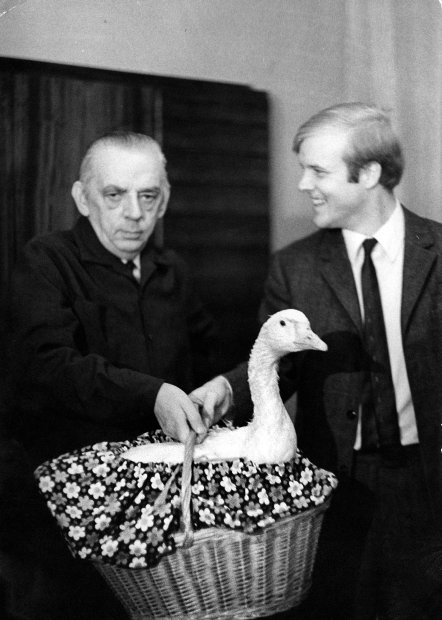
\includegraphics[width=.4\textwidth]{figures/mazur_goose_enflo.jpg}};
	\end{tikzpicture}
	\caption{Nel 1936 Mazur mise in palio un'oca `viva, e grassa' per la risoluzione del problema dell'approssimazione. Nel 1972, Enflo riceve dunque il suo premio.}
\end{figure}

\section{Elementi di teoria spettrale}
\begin{definition}
	Sia $E$ uno spazio di Banach, sia $T:E \to E$ lineare e continuo. Si chiama \defining{insieme risolvente} di $T$ l'insieme
	\begin{equation*}
		\rho(T) = \{\lambda \in \C \suchthat \text{$T-\lambda I$ è biettiva} \}.
	\end{equation*}
	In altre parole,
	\begin{equation*}
		\lambda \in \rho(T) \sse \text{per ogni $y \in E$ esiste $x \in E$ tale che $Tx - \lambda x = y$}.
	\end{equation*}
	Per $\lambda \in \rho(T)$, si dice \defining{operatore risolvente} associato l'operatore $(T-\lambda I)^{-1}$. Infine, si dice \defining{spettro} di $T$ l'insieme
	\begin{equation*}
		\sigma(T) = \C \setminus \rho(T).
	\end{equation*}
	Lo spettro puntuale di $T$ è l'insieme di tutti i suoi autovalori e si indica con $\sigma_p(T)$.
\end{definition}

\begin{remark}
	In dimensione finita, $\sigma = \sigma_p$, mentre in generale $\sigma_p \subseteq \sigma$.
\end{remark}

\begin{theorem}
\label{th:ops_five}
	Sia $E$ spazio di Banach, $T:E \to E$ lineare e continuo.
	Allora $\sigma(T)$ è chiuso e limitato, in particolare $\sigma(T) \subseteq B(0,\|T\|)$.
	Inoltre, se $E$ è complesso allora $\sigma(T) \neq \varnothing$.
\end{theorem}
\begin{proof}
	Per mostrare la chiusura di $\sigma(T)$, proviamo l'apertura di $\rho(T)$.
	Prendiamo allora $\lambda_0 \in \rho(T)$, $\lambda \in \C$ ed $y \in E$. Consideriamo l'equazione
	\begin{equation*}
		(T-\lambda I)(x) = y,
	\end{equation*}
	da cui
	\begin{eqalign*}
		Tx - \lambda x = y\\
		Tx - \lambda_0 x + \lambda_0 x - \lambda x = y\\
		(T-\lambda_0 I)x = y + (\lambda - \lambda_0) x\\
		x = (T-\lambda_0 I)^{-1}(y + (\lambda - \lambda_0)x)\\
		x = (\lambda - \lambda_0)(T-\lambda_0 I)^{-1}x + (T-\lambda_0 I)^{-1} y
	\end{eqalign*}
	che è un'equazione di punto fisso. Per il teorema del punto fisso di Banach--Caccioppoli\footnotemark, affinchè tale punto fisso esista  è sufficiente che l'operatore $(\lambda - \lambda_0)(T-\lambda_0I)^{-1}$ abbia norma strettamente inferiore di $1$, cioè che
	\begin{equation*}
		\lambda - \lambda_0 < \frac1{\|T-\lambda_0I\|}.
	\end{equation*}
	Dunque tutti i $\lambda$ in $B(\lambda_0, 1/\|T-\lambda_0I\|)$ sono risolventi, e quindi $\rho(T)$ è aperto.

	\footnotetext{\begin{theorem*}[Banach--Caccioppoli]
		Ogni contrazione (mappa lipschitziana con costante di Lipschitz $< 1$) di uno spazio metrico completo ammette un punto fisso, che si ottiene come limite della successione delle iterate di un punto qualunque.
	\end{theorem*}
	Il teorema ci permette di concludere che l'Italia in Miniatura ha un punto che è rappresentato da sè stesso. Per trovarlo, basta chiedere al bigliettaio dove sia la biglietteria, e così via.}

	Dimostriamo ora che $\sigma(T) \subseteq B(0, \|T\|)$.
	Sia $\lambda \neq 0$, $y \in E$, si ha
	\begin{eqalign*}
		Tx-\lambda x = y\\
		Tx = \lambda x + y\\
		\frac{Tx}\lambda = x+ \frac{y}\lambda\\
		\frac{Tx}\lambda - \frac{y}\lambda = x
	\end{eqalign*}
	che è ancora un'equazione di punto fisso. Ragionando come sopra, otteniamo che $\lambda \in \rho(T)$ se $\|T/\lambda\| < 1$, cioè se $\lambda > \|T\|$. Ma allora $\sigma(T) \subseteq B(0,\|T\|)$.

	Infine, si può dimostrare che l'operatore che associa $\lambda \in \rho(T)$ al suo operatore risolvente è analitica, e si può dimostrare che $\lim_{|\lambda| \to \infty} (T-\lambda I)^{-1} = 0$ poichè sappiamo che $\rho(T)$ è contenuta nel complementare di una palla. Da ciò segue che $\|T-\lambda I^{-1}\|$ è limitata.
	Ma se $\sigma(T) = \varnothing$, allora $\rho(T) = \C$ e siccome $\lambda \mapsto \|(T-\lambda I)^{-1}\|$ è analitica, dal teorema di Liouville otterremo che è costante. Siccome il limite è nullo, dovrebbe essere costantemente nulla, cioè $T-\lambda I = 0$, assurdo per un operatore invertibile.
\end{proof}

L'ultimo punto è falso in $\R$:

\begin{remark}
	Sia $T:\R^2 \to \R^2$ definito da
	\begin{equation*}
		Tx  = \begin{pmatrix}
			0 & 1\\
			-1 & 0
		\end{pmatrix}x
	\end{equation*}
	Allora $\sigma(T) = \pm i$ mentre è vuoto in $\R$.
\end{remark}

\begin{exercise}
	Sia $T: \ell^2 \to \ell^2$ l'operatore di backshift:
	\begin{equation*}
		T(x_1, x_2, x_3, \ldots) = T(x_2, x_3, \ldots).
	\end{equation*}
	Determinare $\sigma(T)$, $\sigma_p(T)$.

	\textbf{Svolgimento}.
	Si osservi innanzitutto che $\|T\| \leq 1$, d'altro canto $Te_2 = e_1$ dunque $\|T\| = 1$. Segue che $\sigma(T) \subseteq B(0,1)$. Lo spettro puntuale è invece dato da quelle quei $\lambda \in \C$ per cui
	\begin{equation*}
		(x_2, x_3, \ldots) = \lambda (x_1, x_2, \ldots).
	\end{equation*}
	cioè quando
	\begin{equation*}
		x_2 = \lambda x_1, \quad x_3 = \lambda x_2, \ldots
	\end{equation*}
	Allora scelto $x_1 \in \C$, le soluzioni hanno forma
	\begin{equation*}
		x_1 (1, \lambda, \lambda^2, \ldots)
	\end{equation*}
	che per essere in $\ell^2$ debbono avere $|x_1|^2\sum_{n=0}^\infty |\lambda|^{2n} < \infty$, da cui $|\lambda| < 1$. Per cui $\sigma_p(T) = B(0,1)$, ma $\closure{\sigma_p(T)} \subseteq \sigma(T)$, dunque $\sigma(T) = \closure B(0,1)$, ossia
	\begin{equation*}
		\sigma(T) \setminus \sigma_p(T) = \partial B(0,1).
	\end{equation*}
\end{exercise}

\begin{remark}
	Sia $E$ spazio di Banach, e supponiamo che $\dim E = \infty$. Sia inoltre $T:E \to E$ compatto. Allora $0 \in \sigma(T)$ siccome $T$ non è invertibile.
\end{remark}

\begin{theorem}[di Riesz--Schauder]
\label{th:riesz_schauder}
	Sia $E$ spazio di Banach e sia $T:E \to E$ compatto.
	Se $\dim E \lneq \infty$ allora $\sigma(T) = \sigma_p(T)$, mentre se $\dim E = \infty$ allora
	\begin{equation*}
		\sigma(T) = \{0\} \cup \underbrace{\{\lambda_1, \ldots, \lambda_n, \ldots\}}_{\text{autovalori al più numerabile}},
	\end{equation*}
	cioè $T$ ha \defining{spettro discreto} e gli autovalori non nulli hanno molteplicità finite, ossia $\dim \ker(T-\lambda I) \lneq \infty$.
	Inoltre, nel caso $\sigma(T)$ sia infinito, $\lambda_n \conv 0$.
\end{theorem}
\begin{proof}
	Omissis.
\end{proof}

\begin{lemma}
\label{lemma:ops_spectral_selfadjoint}
	Sia $H$ spazio di Hilbert, $T:H \to H$ autoauggiunto.
	Allora
	\begin{enumerate}
		\item gli autovalori di $T$ sono reali,
		\item autovettori relativi ad autovalori distinti sono ortogonali,
		\item e, nel caso $T$ sia compatto e $H\neq \{0\}$, uno tra $\|T\|$ e $-\|T\|$ è un autovalore di $T$.
	\end{enumerate}
\end{lemma}
\begin{proof}
	\leavevmode
	\begin{enumerate}
		\item Sappiamo che per $T$ autoauggiunto, $(Tx,x) \in \R$. D'altra parte da $Tx=\lambda x$ otteniamo che $(Tx,x) = \lambda (x,x)$ è reale, perciò necessariamente $\lambda \in \R$.
		\item Supponiamo che $x$ sia autovettore per $\lambda_1$ e $y$ per $\lambda_2 \neq \lambda_1$. Vale
		\begin{equation*}
			(\lambda_1 x, y) = (Tx, y) = (x, Ty) = (x, \lambda_2 y)
		\end{equation*}
		da cui $(\lambda_1 - \lambda_2)(x,y) = 0$ che implica $(x,y) = 0$ in quanto abbiamo supposto $\lambda_1 \neq \lambda_2$.
		\item Si può dimostrare che se $T$ è autoauggiunto, allora $\|T\| = \sup_{\|x\|=1} |(Tx,x)|$. Nel caso $T$ sia compatto e non banale, allora esiste una successione $\{x_n\}_{n \in \N}$ in $H$, di norma unitaria, tale che $|(Tx_n,x_n)| \conv \|T\|$.
		Salvo passare ad una sottosuccessione, $(Tx_n, x_n) \conv \|T\|$ o $-\|T\|$, Chiamiamo questo limite $\mu$. Si ha
		\begin{eqalign*}
			\|Tx_n - \mu x_n\|^2  &= \|Tx_n\|^2 - 2 \mu \Re{Tx_n, x_n} + \mu^2 \|x_n\|^2\\
			&\leq \|T\|^2 - 2\mu \underbrace{(Tx_n, x_n)}_{\conv \mu} + \mu^2 \conv 0.
		\end{eqalign*}
		Per compattezza di $T$, a meno di passare ad una sottosuccessione, $Tx_n$ converge. Allora la convergenza di $Tx_n$ implica la convergenza di $\mu x_n$ (carabinieri). Segue che $x_n \conv x$, per cui $Tx_n - \mu x_n \conv Tx - \mu x = 0$, e $\|x\| =1$ dunque $x \neq 0$.
	\end{enumerate}
\end{proof}

Il seguente è un teorema spettrale per gli operatori compatti. Ne esiste una versione analoga per operatori non compatti, dimostrata da Stone, ed infine per operatori non limitati, dimostrato da Von Neumann.

\begin{theorem}[Il famoso teorema di Hilbert--Schmidt]
	Sia $T:H \to H$ un operatore compatto ed autoauggiunto su uno spazio di Hilbert $H$.
	Allora esiste una successione $\{u_n\}_{n \in \N}$ in $H$ di autovettori associati agli autovalori non nulli di $T$, tale che
	\begin{enumerate}
		\item $\{u_n\}_{n \in \N}$ è una base hilbertiana per $\closure{\im T}$.
		\item Se $\{\lambda_n\}_{n \in \N}$ è la successione degli autovalori associati agli $\{u_n\}_{n \in \N}$, ognuno ripetuto tante volte quanto è la sua molteplicità, allora
		\begin{equation}
		\label{eq:hilbert_schmidt}
			Tx = \sum_{n=1}^\infty \lambda_n\, (x,u_n)\,u_n.
		\end{equation}
	\end{enumerate}
\end{theorem}
\begin{remark}
	La~\eqref{eq:hilbert_schmidt} esprime il fatto che $T$ è diagonale rispetto alla base $\{u_n\}_{n \in \N}$!
\end{remark}
\begin{proof}
	Ricordiamo che $\closure{\im T} = (\ker T)^\perp$, e $H= \ker T \oplus \closure{\im T}$. Sia
	\begin{equation*}
		\Lambda = \{ \text{autovalori non nulli di $T$} \}
	\end{equation*}
	Abbiamo visto che $\dim \ker (T -\lambda I) = n_\lambda \lneq \infty$, per ogni autovalore $\lambda in \Lambda$. Dunque possiamo mettere insieme un insieme ortonormale numerabile andando a pescare una base ortonormale (finita) per ogni autospazio.
	Sia $U=\{u_n\}_{n \in \N}$ tale insieme, vogliamo provare che $\closure{\langle U \rangle} = \closure{\im T}$.
	È banale che $U \subset \im T$ ($Tx = \lambda x \implies x = T(x/\lambda) \in \im T$).
	Invece, supponiamo per assurdo che $\closure{\langle U \rangle } \subsetneq \closure{\im T}$. Siccome $\closure{\im T}$ è uno spazio di Hilbert, possiamo decomporlo come $\closure{\langle U \rangle} \oplus \closure{\langle U \rangle}^\perp$.
	Osserviamo che $T$ fissa $U^\perp$. Se $x \in U^\perp$ infatti, allora per ogni $y \in U$
	\begin{equation}
		(Tx,y) = (x,Ty) = (x, \lambda y) = \underbrace{\lambda}_{\in \R} \underbrace{(x,y)}_{x \perp y} = 0.
	\end{equation}
	Siccome $T$ è compatto ed autoauggiunto, e abbiamo supposto che $\langle U \rangle^\perp$ sia diverso da $\{0\}$, allora dal Lemma~\ref{lemma:ops_spectral_selfadjoint} otteniamo che esiste $u \in \closure{\langle U \rangle}^\perp$ autovettore non nullo di $T$ associato a $\pm \|T\vert_{\closure{\langle U \rangle}^\perp}\|$. Ciò contraddice la massimalità di $U$, e dunque $\closure{\langle U \rangle} = \closure{\im T}$, e quest'ultimo spazio è hilbertiano.

	Sia $x \in H$, siccome $Tx \in \im T$, dal punto precedente (e per il teorema di Fourier) sappiamo che
	\begin{equation*}
		Tx = \sum_{n=1}^\infty (Tx, u_n)\,u_n.
	\end{equation*}
	Infine,
	\begin{equation*}
		(Tx, u_n) = (x, Tu_n) = (x, \lambda_n u_n) = \lambda_n (x, u_n)
	\end{equation*}
	e ciò conclude la dimostrazione.
\end{proof}

\begin{corollary}
	Se $T:H \to H$ è compatto ed autoauggiunto, allora $H$ possiede una base hilbertiana di autovettori di $T$.
\end{corollary}
\begin{proof}
	Infatti $H = \ker T \oplus \closure{\im T}$. Per il teorema precedente, $\closure{\im T}$ ha una base hilbertiana numerabile di autovettore, mentre $\ker T$ ha una base hilbertiana in quanto sottospazio chiuso in uno spazio di Hilbert. Siccome $\ker T$ è un autospazio per $T$, la tesi è provata.
\end{proof}

\begin{remark}
	Si noti che la decomposizione $H = \ker T \oplus \closure{\im T}$ associata ad un operatore compatto ed autoauggiunto esibisce $H$ diviso in una parte separabile (l'immagine, che ha una base hilbertiana numerabile) ed una non separabile. Chiaramente $\closure{\im T}$ non è necessariamente massimale.
\end{remark}

\begin{theorem}[dell'alternativa di Fredholm]
	Sia $T:H \to H$ compatto e autoauggiunto. Consideriamo le seguenti equazioni:
	\begin{equation*}
		(1)\ x - Tx = 0, \qquad (2)\ x-Tx = y.
	\end{equation*}
	Allora vale una e una sola delle seguenti alternative:
	\begin{enumerate}
		\item La $(1)$ ha solo la soluzione nulla, nel qual caso $(2)$ ha una e una sola soluzione per ogni $y \in H$.
		\item La $(1)$ ha soluzione non nulla, nel qual caso $(2)$ ha soluzione se e solo se $y$ è ortogonale a tutte le soluzioni di $(1)$.
		Inoltre se vi è una soluzione allora ce ne sono infinite.
		Infine, lo spazio di tali soluzioni è chiuso.
	\end{enumerate}
\end{theorem}
\begin{proof}
	Si assuma che $(1)$ abbia solo la soluzione nulla. Ciò significa che $1 \notin \sigma_p(T)$, e dunque $1 \notin \sigma(T)$, e quindi $I-T$ è invertibile e la $(2)$ ha sempre una soluzione unica.

	Supponiamo invece che $(1)$ abbia soluzione non nulle, da cui $1 \in \sigma_p(T)$ e $\ker (I-T) \neq \{0\}$. Allora $H = \ker (I-T) \oplus \closure{\im (I-T)}$. Allora se $y \in \im(I-T)$, $y \perp \ker (I-T)$, cioè che se la $(2)$ ha soluzione per $y$ allora $y$ è ortogonale alle soluzioni di $(1)$.
	Proviamo ora che se $y \in (\ker(I-T))^\perp$, allora $y \in \im(I-T)$. Da questo discende anche che $\im(I-T)$ è chiuso, in quanto complemento ortogonale.
	Usiamo Hilbert--Schmidt per ottenere una base hilbertiana di autovalori di $T$ per $\closure{\im T}$. Per cui nella $(2)$ poniamo
	\begin{equation*}
		x = x_0 + x_1, \quad y=y_0+y_1
	\end{equation*}
	dove $x_0,y_0 \in \ker T$ e $x_1,y_1 \in \closure{\im T}$. Del resto
	\begin{equation*}
		x = x_0 + \sum_{n=1}^\infty (x, u_n)\,u_n, \qquad y = y_0 + \sum_{n=1}^\infty (y, u_n)\,u_n
	\end{equation*}
	e l'equazione diventa
	\begin{equation*}
		x_0 + \sum_{n=1}^\infty (x, u_n)\,u_n - \sum_{n=1}^\infty \lambda_n (x,u_n) u_n = y_0 + \sum_{n=1}^\infty (y, u_n)\,u_n
	\end{equation*}
	cioè
	\begin{equation*}
		(2) \iff
		\begin{cases}
			x_0 = y_0,\\
			(1-\lambda_n)(x,u_n) = (y,u_n)
		\end{cases}
	\end{equation*}
	Quindi se $\lambda_n =1$, $(y,u_n) = 0$. Ma infatti $y \in \ker(I-T)$, che è l'autospazio relativo a $1$.
	Se invece $\lambda_n \neq 1$, si ottiene
	\begin{equation*}
		(x,u_n) = \frac{(y,u_n)}{1-\lambda_n}
	\end{equation*}
	che mi permette di ottenere $x$, siccome la successione $(y,u_n)/(1-\lambda_n)$ è in $\ell^2$ (perchè $\lambda_n \conv 0$, quindi $1-\lambda_n$ è in $\ell^\infty$, ed $(y,u_n) \in \ell^2$).
\end{proof}


	\nocite{*}
	\printbibliography[heading=bibintoc]
\end{document}
